\documentclass[12pt]{article}
\usepackage[
    % top=10mm,
    % bottom=10mm,
    % left=10mm,
    % right=10mm,
    marginparwidth=0mm,
    marginparsep=0mm,
    % headheight=15pt,
    centering,
    % showframe,
    includefoot,
    % includehead
]{geometry}

\usepackage{tikz}
\usepackage{tikz-cd}
\usepackage{multicol}
\usepackage{hyperref}
\usepackage{breqn}

\usetikzlibrary{shapes.geometric}

\hypersetup{
    colorlinks=false,
    linktoc=all,
}

\renewcommand{\date}[1]{\underline{\bf #1}}

\def\eps{\varepsilon}
\def\range{\text{Range}}
\def\proj{\text{proj}}
\def\Stab{\text{Stab}}
\def\Isom{\text{Isom}}
\def\Perm{\text{Perm}}
\def\Syl{\text{Syl}}

\newcommand{\GCD}{\text{GCD}}
\def\RowSpace{\text{RowSpace}}
\def\ColSpace{\text{ColSpace}}
\def\trace{\text{trace}}
\def\Ann{\text{Ann}}
\def\sgn{\text{sgn}}
\def\B{\mathcal B}
\def\P{\mathcal P}
\newcommand{\lcm}{\text{lcm}}
% \newcommand{\Aut}{\text{Aut}}

\def\phi{\varphi}
\def\sgn{\text{sgn}}
\def\image{\text{image}}

\def\Tinv{$T$-invariant}


% create a command for TODOs
\newcommand{\TODO}{\color{red}\textbf{TODO}\color{black}}

\newcommand*{\xdash}[1][3em]{\color{darkgray}\rule[0.5ex]{#1}{0.55pt}\color{black}}

\newcommand{\ip}[2]{\left( #1 \mid #2 \right)}

\newcommand{\lr}[1]{\langle #1 \rangle}

\renewcommand{\char}{\text{char}}

% preamble
\usepackage{amssymb}
\usepackage{amsmath, amsthm}
\usepackage{xcolor}
\usepackage{fancyhdr}
\usepackage{enumitem}
\usepackage{mathtools}
\usepackage{framed}
\usepackage{parskip}
\usepackage{graphicx}
\usepackage{chngcntr}
\usepackage{float}
\usepackage{listings}
\usepackage{inconsolata}
\usepackage{transparent}
\usepackage{tikz}


% \input xypic (for commutative diagrams)
% \include{mssymb}

\def\A{{\mathbb A}}
\def\P{{\mathbb P}}
\def\N{{\mathbb N}}
\def\Z{{\mathbb Z}}
\def\Q{{\mathbb Q}}
\def\R{{\mathbb R}}
\def\C{{\mathbb C}}
\def\F{{\mathbb F}}
\def\O{{\cal O}}
\let\sec\S
\let\S\relax
\def\S{{\mathfrak S}}
\def\g{{\mathfrak g}}
\def\p{{\mathfrak p}}
\def\h{{\mathfrak h}}
\def\n{{\mathfrak n}}
\def\v{{\mathfrak v}}
\def\m{{\mathfrak m}}
\def\a{{\alpha}}


\newcommand{\skipline}{\vspace{\baselineskip}}
\newcommand{\dis}{\displaystyle}
\newcommand{\noin}{\noindent}


% remove all paragraph indents
\setlength{\parindent}{0pt}

% Figure counter include section
\counterwithin{figure}{section}

% Cleaner figures
\newcommand{\fig}[3][0.4]{
  \begin{figure}[H]
    \centering
    \includegraphics[width=#1\textwidth, keepaspectratio]{#2}
    \caption{#3}
  \end{figure}
}

% Parens, Brackets, Bars, and Braces
\newcommand{\parens}[1]{ \left(#1\right) }
\newcommand{\bracks}[1]{ \left[#1\right] }
\newcommand{\braces}[1]{ \left\{#1\right\} }
\newcommand{\abs}[1]{ \left|#1\right| }
\newcommand{\floor}[1]{ \left\lfloor#1\right\rfloor }
\newcommand{\ceil}[1]{ \left\lceil#1\right\rceil }

% Mathematical notation


\newcommand{\Span}{\mathrm{Span}}
\newcommand{\Range}{\mathrm{Range}}
\newcommand{\Null}{\mathrm{Null}}
\newcommand{\Rank}{\mathrm{Rank}}
\newcommand{\rank}{\mathrm{rank}}
\newcommand{\Nullity}{\mathrm{Nullity}}
\newcommand{\nullity}{\mathrm{nullity}}
\newcommand{\longhookrightarrow}{\lhook\joinrel\relbar\joinrel\rightarrow}
\newcommand{\la}{\leftarrow}
\newcommand{\ra}{\rightarrow}
\newcommand{\La}{\Leftarrow}
\newcommand{\Ra}{\Rightarrow}
\newcommand{\dbar}{\overline{\partial}}
\newcommand{\gequ}{\geqslant}
\newcommand{\lequ}{\leqslant}
\newcommand{\Hom}{\mathrm{Hom}}
\newcommand{\End}{\mathrm{End}}
\newcommand{\Aut}{\mathrm{Aut}}
\newcommand{\Coker}{\mathrm{Coker}}
\newcommand{\Row}{\mathrm{Row}}
\newcommand{\Ker}{\mathrm{Ker}}
\newcommand{\Tr}{\mathrm{Tr}}
\newcommand{\Id}{\mathrm{Id}}
% \newcommand{\mod}{\mathrm{mod }}
\newcommand{\un}{\underline}
\newcommand{\ov}{\overline}
\newcommand{\wt}{\widetilde}
\newcommand{\wh}{\widehat}
\newcommand{\pr}{\prime}
\newcommand{\rk}{\mathrm{rk}}
\newcommand{\im}{\mathrm{Im}}

% Linear Algebra

\newcommand{\lind}{linearly independent}
\newcommand{\ldep}{linearly dependent}
\renewcommand{\vec}[1]{
  {\bf #1}
}
\newcommand{\lincomb}[3]{
  #1_{1}#2_{1} + #1_{2}#2_{2} + \cdots + #1_{#3}#2_{#3}
}
\newcommand{\neglincomb}[3]{
  -#1_{1}#2_{1} - #1_{2}#2_{2} - \cdots - #1_{#3}#2_{#3}
}
\newcommand{\constants}[2]{
  #1_{1}, #1_{2}, \cdots, #1_{#2}
}
\newcommand{\constantsz}[2]{
  #1_{0}, \constants{#1}{#2}
}

% Analysis
\newcommand{\limfty}[1]{\lim_{#1 \to \infty}}
\newcommand{\seq}[2]{\{#1_{#2}\}_{#2 \in \N}}
\newcommand{\sseq}[3]{\{#1_{#2_{#3}}\}_{#3 \in \N}}
\newcommand{\chep}{Let $\epsilon > 0$}

% Category Theory
\newcommand{\catC}{\mathcal{C}}
\newcommand{\catD}{\mathcal{D}}
\newcommand{\functF}{\mathcal{F}}
\newcommand{\functG}{\mathcal{G}}
\newcommand{\functI}{\mathcal{I}}
\newcommand{\functU}{\mathcal{U}}

\newcommand{\op}[1]{#1^{\mathrm{op}}}
\newcommand{\Obj}{\mathrm{Obj}}

\newcommand{\Set}{\mathbf{Set}}
\newcommand{\Grp}{\mathbf{Grp}}
\newcommand{\Top}{\mathbf{Top}}
\newcommand{\cRing}{\mathbf{cRing}}
\newcommand{\BanAnaMan}{\mathbf{BanAnaMan}}
\newcommand{\FinSet}{\mathbf{FinSet}}
\newcommand{\Vect}{\mathbf{Vect}}
\newcommand{\Two}{\mathbf{2}}


% ================= %
% Headers & Footers
% ================= %
\pagestyle{fancy}
\fancyhf{}
\newcommand{\intros}[3]{
  \lhead{\textbf{#1} {#2}}
  \rhead{#3}}
\rfoot{\thepage}
\renewcommand{\headrulewidth}{0pt}



% ================= %
%       Utils
% ================= %
\newcommand{\induction}[3]{
  \textbf{Base Case}. #1 \\
  \textbf{Inductive Hypothesis}. \\ #2 \\
  \textbf{Inductive Step}. \\ #3
}



% Used to list all problems on homework
\newcommand{\problems}[1]{
  \medskip \noin
  {\bf Problems}

  #1

  \medskip{}
}


% When prof does Question/Answer styling
\newcommand{\qna}[2]{
  {\bf Question}: #1

  {\bf Answer}: #2
}


% augmented matrices
\makeatletter
\renewcommand*\env@matrix[1][*\c@MaxMatrixCols c]{%
  \hskip -\arraycolsep
  \let\@ifnextchar\new@ifnextchar
  \array{#1}}
\makeatother


\newcommand\restr[2]{{% we make the whole thing an ordinary symbol
  \left.\kern-\nulldelimiterspace % automatically resize the bar with \right
  #1 % the function
  \littletaller % pretend it's a little taller at normal size
  \right|_{#2} % this is the delimiter
  }}

\newcommand{\littletaller}{\mathchoice{\vphantom{\big|}}{}{}{}}

% ================= %
%      Box Meta
% ================= %

% #2 - FG Color
% #3 - BG Color
\newenvironment{fancyleftbar}[3][\hsize]
{%
    \def\FrameCommand
    {%
        {\color{#2}\vrule width 3pt}%
        \hspace{0pt}%must no space.
        \fboxsep=\FrameSep\colorbox{#3}%
    }%
    \MakeFramed{\hsize#1\advance\hsize-\width\FrameRestore}%
}
{\endMakeFramed}

\newenvironment{simpleleftbar}[3][\hsize]
{%
    \def\FrameCommand
    {%
        {\vrule width 0.5pt}%
        \hspace{3pt}
        \fboxsep=\FrameSep%
    }%
    \MakeFramed{\hsize#1\advance\hsize-\width\FrameRestore}%
}
{\endMakeFramed}

% Used to allow the color argument to pass through the environment%
\newsavebox{\boxqed} 

% #1 - Header
% #2 - FG Color
% #3 - BG Color
\newenvironment{fancybox}[3]{
  \sbox\boxqed{\textcolor{#2}{$\blacksquare$}}
  \begin{fancyleftbar}{#2}{#3}

  \noin
  #1
  % {\large \bf \underline{#1}}
  \smallskip\noin \\
}
{

  \medskip
  \noin
  \usebox\boxqed

  \end{fancyleftbar}
}

% #1 - Text header
% #2 - Outer Text
% #3 - Inner Text
% #4 - Inner Header
% #5 - FG Color
% #6 - Background Color
\newcommand{\boxmeta}[6]{
  #1
  % {\small\sc\uppercase{#1}}

  #2

  \begin{fancybox}{#4}{#5}{#6}
    \noin
    #3
  \end{fancybox}
}

% #1 - Title
% #2 - FG Color
% #3 - BG Color
% #4 - Inner Text
\newcommand{\baronly}[4]{
  \begin{simpleleftbar}{#2}{#3}
    {\bf #1}.

    #4
  \end{simpleleftbar}
}

% ================= %
%     Box Colors
% ================= %

\definecolor{theorem_fg}{HTML}{EABAC3}
\definecolor{theorem_bg}{HTML}{F9EEF0}

\definecolor{problem_fg}{HTML}{ABABAB}
\definecolor{problem_bg}{HTML}{EDEDED}

\definecolor{lemma_fg}{HTML}{D0C97D}
\definecolor{lemma_bg}{HTML}{FCF9DB}

\definecolor{prop_fg}{HTML}{7DDB89}
\definecolor{prop_bg}{HTML}{D7FADB}

\definecolor{defn_fg}{HTML}{83D4CF}
\definecolor{defn_bg}{HTML}{E7FCFB}

\definecolor{lst_bg}{HTML}{EFF6F8}
\definecolor{lst_fg}{HTML}{475857}

\definecolor{btw_fg}{HTML}{5A5A5A}

% ================= %
%     Box Envs
% ================= %

\newcommand{\Definition}[2]{
                              \boxmeta{}{}{#2}{{\it Definition}. {\bf\underline{#1}}}{defn_fg}{defn_bg}
                            }

\newcommand{\Theorem}[2]{
  \boxmeta{{\bf Theorem.}}{#1}{#2}{{\bf Proof.}}{theorem_fg}{theorem_bg}
}

\newcommand{\NamedTheorem}[3]{
  \boxmeta{#1}{#2}{#3}{Proof}{theorem_fg}{theorem_bg}
}

\newcommand{\Problem}[3]{
  \boxmeta{Problem #1}{#2}{#3}{Solution}{problem_fg}{problem_bg}
}

\newcommand{\Example}[2]{
  \boxmeta{Example}{#1}{#2}{}{problem_fg}{problem_bg}
}

\newcommand{\Lemma}[2]{
  \boxmeta{{\bf Lemma.}}{#1}{#2}{{\bf Proof.}}{lemma_fg}{lemma_bg}
}

\newcommand{\NamedLemma}[3]{
  \boxmeta{#1}{#2}{#3}{Proof}{lemma_fg}{lemma_bg}
}

\newcommand{\Corollary}[2]{
  \boxmeta{Corollary}{#1}{#2}{Proof}{lemma_fg}{lemma_bg}
}

\newcommand{\Proposition}[2]{
  \boxmeta{Proposition}{#1}{#2}{Proof}{prop_fg}{prop_bg}
}

% ================== %
%      Bar Only
% ================== %

\newcommand{\definition}[1]{
  \baronly{Definition}{defn_fg}{defn_bg}{#1}
}

\newcommand{\theorem}[1]{
  \baronly{Theorem}{theorem_fg}{theorem_bg}{#1}
}

\newcommand{\example}[1]{
  \baronly{Example}{problem_fg}{problem_bg}{#1}
}

\newcommand{\remark}[1]{
  \baronly{Remark}{problem_fg}{problem_bg}{#1}
}

\newcommand{\note}[1]{
  \medskip
  \baronly{Note}{problem_fg}{problem_bg}{#1}
}

\newcommand{\btw}[1]{
  {\bf Author Note}.

  \begin{color}{btw_fg}
    #1
  \end{color}
}

\newcommand{\sidenote}[1]{
  {\bf Side Note}.

  \boxmeta{}{}{#1}{}{problem_fg}{problem_bg}
}



% graphs
\def\deg{\text{deg}}
\def\indeg{\text{indeg}}
\def\outdeg{\text{outdeg}}

% big O notation
\def\O{\mathcal O}

% define parent
\def\pr{\text{pr}}

% define incomplete commands
\def\TODO{\color{red}\textbf{TODO}\color{black}\,}
\def\QUESTION{\color{red}\textbf{QUESTION}\color{black}\,}



% listings settings
\lstset{
  % general styles
  backgroundcolor=\color{lst_bg},
  numbers=left,
  numberstyle=\color{lst_fg}\ttfamily\textbf,
  numbersep=3mm,
  frame=l,
  framesep=7mm,
  framexleftmargin=1.5mm,
  fillcolor=\color{lst_bg},
  rulecolor=\color{lst_bg},
  xleftmargin=9mm,
  % keyword styles
  keywordstyle=[1]\textbf,
  keywordstyle=[2]\textit,
  keywordstyle=[3]\textbf\textit,
  keywords=[1]{let, for, while, not, if, else, then, do, end, return},
  keywords=[2]{if, condition},
  keywords=[3]{do},
  mathescape=true, % enable math mode in listings
  columns=fullflexible,
  basicstyle=\ttfamily % this fond looks a bit better than the default
}



% colors used in proof boxes
\definecolor{proof_fg}{HTML}{ABABAB}
\definecolor{proof_bg}{HTML}{EDEDED}

\def\acts{\curvearrowright}


% box solutions
\newenvironment{solution}{
  \begin{leftbar}

  \noin
  {\large \sc solution} \\
}
{

  \medskip
  \noin
  \textcolor{proof_fg}{$\blacksquare$}

  \end{leftbar}
}



% style a problem and solution
\newcommand{\prob}[3]{
  \bigskip \bigskip \noin
  {\Large\sc Problem #1}

  \medskip\noin
  #2

  \begin{solution}
    \noin
    #3
  \end{solution}
}

\renewcommand{\mod}[1]{
  \text{ (mod $#1$) }
}

\def\mat{\text{Mat}}
\def\gl{\text{GL}}
\def\sl{\text{SL}}



\begin{document}

\tableofcontents

\date{Wed. 24 Jan 2024}

\note {
All info for the class is available on the canvas page.
Notes from the prof are written on the iPad, and PDFs will be provided after
each class. Despite this taking notes is helpful.

Offices are hours are Tuesdays in person, and Thursdays on Zoom. Hours may
vary.

A text for this class is not {\it required}. Technically, we are using
Fraleigh's {\it A first course in Abstract Algebra}

No quizzes in this class, weekly Homeworks except on Exam weeks, two
midterms, and one final.

Readings on the class schedule are not additional, it's for people that need
extra material, or people that missed that day.
}

\section{Introduction - Sets and Relations}

\subsection{Sets}

\definition{
	A {\bf Set}. is a well-defined collection of objects called {\it elements}.

	$a \in A$ means ``$A$ is a set, $a$ is an element of a set, and $a$ is in
	$A$.
}

Examples of sets are

\begin{itemize}
	\item $\Z$ - The set of all integers, positive, negative, and zero
	\item $\N$ - The set of natural numbers, $0, 1, 2, \dots$. {\bf In this
			      class, $\N$ starts with $1$.}
	\item $\Q$ - The set of rational numbers.
	\item $\R$ - The set of real numbers.
	\item $\C$ - The set of complex numbers.
	\item $\{1, 2, 3, 4\}$
	\item $\{a \in \Z \mid a > 2 \}$. This is a set of integers {\it such that} $a
		      > 2$.
	\item $\varnothing$ - The empty set.
	\item $\text{GLn}(\R)$ - The set of $n \times n$ invertible matrices with real
	      entries. (GL stands for ``General Linear".)
	\item $C(\R)$ - The set of continuous functions $f: \R \to \R$.
\end{itemize}

\definition{
	A set $A$ is a {\bf subset} of a set $B$ if

	\[
		\forall x \in A, x \in B
	\]

	In other words, everything in $A$ is also in $B$. As notation, we can say
	either $A \subseteq B$ or $A \subset B$.

	A {\bf proper} subset is $A \subset B$ but $A \ne B$. Just write $A
		\subsetneq B$.
}

For example, $\N \subseteq \Z \subseteq \Q \subseteq \R \subseteq \C$. And,
importantly, $\varnothing \subseteq A$ for all sets $A$. In other words, the
empty set is a subset of {\it all} sets.

Two sets are equal if $A = B$, or $A \subseteq B$ {\it and} $B \subseteq A$.
This is often how you prove set equality.

\subsubsection{Set Operations}

We have four main operations.

\begin{itemize}
	\item {\bf Union}: $A \cup B = \{x \mid x \in A \text{ or } x \in B \}$.
	\item {\bf Intersection}: $A \cap B = \{ x \mid x \in A \text{ and } x \in B \}$.
	\item {\bf Product}: $A \times B = \{(a, b) \mid a \in A, b \in B \}$.
	\item {\bf Difference}: $A \setminus B = \{x \mid x \in A \text{ and } x \not\in B\}$
\end{itemize}

Two sets are {\bf disjoint} if $A \cap B = \varnothing$.

If we're working in a particular {\it universe} $U$ (i.e. all sets are subsets
of the universal set $U$) then the {\it complement} of $A$ is $A^c = \{x \mid x
	\in U \text{ and } x \not\in A \}$.

\subsection{Relations}

\definition {
	A {\bf relation} between sets $A$ and $B$ is a subset $R \subseteq A \times
		B$.
}

If $(a, b) \in R$, then we say that ``$a$ is related to $b$", or we write
$aRb$, or $a \sim b$.

\example {
	$R \subseteq \{1, 2, 3\} \times \{2, 3, 4\}$. $R = \{(1, 3), (2, 2), (3, 4) \}$
}

\note {
	Relations might not be reflexive! If $(a, b) \in R$, that means $a$ is
	related to $b$, but it might not be the case that $(b, a) \in R$. In other
	words, the reverse may not be true!
}

Another example might be $R \subseteq \R \times \R$, with $R = \{(x, x^3) \mid x
	\in \R \}$. Oh look! We just rewrote $f(x) = x^3$, so functions are relations.

\definition {
	A {\bf partition} of a set $A$ is a collection of {\it disjoint} subsets
	whose union is $A$.

	Another way to think of this is that any element of $A$ is in one and only
	one of its partitions.
}

An example of this might be the partition

\[
	A = \Z = \{x \in \Z \mid x < 0 \} \cup \{ 0 \} \cup \{ x \in \Z \mid x > 0 \}
\]

is a partition of $\Z$ into 3 sets.

Another example might be $A = \R$, subsets are $\{ x \}$ for each $x \in \R$.

Another, maybe more interesting example might be the following.

\example {
Fix $n \in \N$, $n \ge 2$. Let

\begin{itemize}
	\item $\bar 0 = \{x \in \Z \mid x \text{ is divisible by } n \}$.
	\item $\bar 1 = \{x \in \Z \mid x - 1 \text{ is divisible by } n \}$.
	\item $\bar 2 = \{x \in \Z \mid x - 2 \text{ is divisible by } n \}$. On and
	      on until...
	\item $\overline{n - 1} = \{x \in \Z \mid x - (n - 1) \text{ is divisible by } n
		      \}$.
\end{itemize}

{\bf Claim}: This partitions $\Z$ into in $n$ subsets.

}

\date{Fri. 26 Jan 2024}

Let's go back to relations, which we put aside to talk about partitions.

\definition {
	A relation $A \subseteq A \times A$ is called an {\bf equivalence relation}
	if it satisfies 3 properties

	\begin{enumerate}
		\item {\bf Reflexivity}: $aRa$ for all $a \in A$.
		\item {\bf Symmetry}: $aRb$ if and only if $bRa$.
		\item {\bf Transitivity}: If $aRb$ and $bRc$, then $aRc$.
	\end{enumerate}
}

The key idea is that equivalence relations on $A$ are {\it the same} as
partitions of $A$. What's going on here?

From an equivalence relation: If $b$ is related to $b$, put them in the same
set. Because of symmetry of equivalence relations, order of elements in the
set doesn't matter.

Conversely, given a partition say $aRb \Leftrightarrow bRa$ are in the same
subset.

\note {
	We'll be talking a lot about partitions and equivalence relations in this
	class.
}

Now we move on to the next step in our intro: functions.

\subsection{Functions}

A function $f: A \to B$ is a relation $R_f \subseteq A \times B$ such that,
for all $a \in A$, there is a {\it unique} $b \in B$ such that $aRb$.
Effectively, this means that

\begin{enumerate}
	\item We pass the vertical line test.
	\item The function is defined over its entire domain.
\end{enumerate}

Which are the properties we expect of functions!

\example {
	Let $f: \R \to \R$, with $R_f = \{(x, x^3) \mid x \in \R \}$. We write $f(a)$
	for the value $b$ where $(a, b) \in R_f$.
}

Given a function $f: A \to B$. We say that

\begin{itemize}
	\item $A$ is the {\it domain}.
	\item $B$ is the {\it codomain}.
	\item The {\it range} is a {\it subset} of the codomain, only where $f$
	      outputs values.
\end{itemize}

The $+$ operation is a function $+: \R \to \R$, also written as $(a, b)
	\mapsto a + b$. The multiplication operation $\times: \R \times \R \to \R$,
also written as $(a, b) \to ab$. These are binary operations, very useful in
Group Theory.

\definition {
	A {\bf binary operation} on a set $A$ is a function $f: A \times A \to A$.
	Its an operation on two inputs that outputs one thing.
}

\note {
	A dot product does not count here! Because the output of the dot
	product does not come from the same set as the input.
}

To do more complicated things in real life (such as $a + b + c$), we must
parenthesize.

\[
	f(a, f(b, c)) \text{ or } f(f(a, b), c)
\]

Of course this doesn't matter for addition in particular, but it might for
other binary operators!

\example {
	Fix $n \ge 2$ and consider $\Z_n = \{\bar 0, \bar 1, \dots, \overline{n - 1}
		\}$ (Note that this is a set of sets!)

	We want to come up with binary operations on this set. We have

	\begin{enumerate}
		\item Addition: $+: \Z_n \times \Z_n \to \Z_n$, defined as $(\bar a, \bar
			      b) \mapsto \overline{a + b}$.

		      But this isn't well-defined! For instance, what happens if $a + b$
		      exceeds $n$? To fix this, let's add the following condition:

		      Let $\bar x = \bar y$ if $x, y$ are in the same subset of partitions.
		      (i.e. They have the same remainder mod $n$.)

		      \qna {
			      Is this a well-defined binary operations?
		      }
		      {
			      Yes! But we must check that it doesn't matter how we define our
			      inputs.
		      }

		\item Multiplication: $\times: \Z_n \times \Z_n \to \Z_n$, defined as
		      $(\bar a, \bar b) \mapsto \overline{ab}$
	\end{enumerate}
}

\note {
	We also write $x \equiv y \mod{n} $ if $\bar x = \bar y$.
}

Now we're ready to jump in.

\section{Properties of Operations on R}

Let's look at the properties of $(\R, +)$ and $(\R \setminus \{0\}, \times)$.

\begin{multicols}{2}
	$(\R, +)$

	\begin{enumerate}
		\item {\bf Associativity}: $a + (b + c) = (a + b) + c$

		\item {\bf Identity}: $a + 0 = a$

		\item {\bf Inverses}: $a + (-a) = (-a) + a = 0$

		\item {\bf Commutativity}: $a + b = b + a$
	\end{enumerate}

	$(\R \setminus \{0\}, \times)$

	\begin{enumerate}
		\item {\bf Associativity}: $a \times (b \times c) = (a \times b) \times c$

		\item {\bf Identity}: $a \times 1 = a$.

		\item {\bf Inverses}: $a \times (1/a) = (1/a) \times a = 1$

		\item {\bf Commutativity}: $a \times b = b \times a$
	\end{enumerate}
\end{multicols}

\definition {
	We say that a binary operation $p: A \times A \to A$ is {\bf associative} if

	\[
		p(a, p(b, c)) = p(p(a, b), c)
	\]

	for any $a, b, c \in A$. In other words, how we parenthesize doesn't matter.
}

\definition {
	We say that a binary operation $p: A \times A \to A$ has an {\bf identity} if

	\[
		p(a, e) = p(e, a) = a
	\]

	for any $a \in A$.
}

\definition {
	We say that a binary operation $p: A \times A \to A$ has a {\bf inverses} if

	\begin{enumerate}
		\item It has an identity element $e$ (otherwise identity is meaningless!)

		\item
		      \[
			      p(a, b) = p(b, a) = e
		      \]

		      for any $a \in A$ and some $b \in A$.
	\end{enumerate}

	We usually write $b$ as $a^{-1}$.
}

\definition {
	We say that a binary operation $p: A \times A \to A$ is {\bf commutative} if

	\[
		p(a, b) = p(b, a)
	\]

	for any $a, b \in A$.
}

Let's look at properties of $(\Z_n, +)$ and $(\Z_n, \times)$.

$(\Z_n, +)$

\begin{enumerate}
	\item Is Associative.
	\item Has an identity: $0$.
	\item Has an inverse: $\overline{(-a)}$ for any $\bar a$.
	\item Is Commutative: We can move elements around.
\end{enumerate}

$(\Z_n, \times)$

\begin{enumerate}
	\item Is Associative
	\item Has an identity: $1$.
	\item {\bf Does not} have an inverse! Because $\bar 0$ is still there, we
	      have no inverse.
	\item Is Commutative: We can move elements around. In this case, $\bar a
		      \bar b = \overline{ab} = \overline{ba} = \bar b \bar a$.
\end{enumerate}

\qna {
	If we instead looked at $(\Z_n \setminus \{ 0 \}, \times)$, would there be
	inverses?
}
{
	We've messed the whole thing up! This is not even an binary operation
	anymore. Since we don't have $\bar 0$, what does $\bar 2 + \bar 2$ even mean
	now, if $n = 4$?

	We'll study this more in about a week.
}

Let's look at matrices. $A = \mat_n(\R)$ be the set of $n \times n$ matrices
with real elements, with the binary operation being matrix multiplication.
Let's look at its properties.

\begin{enumerate}
	\item Its associative.
	\item It has an identity.
	\item It {\bf does not} have an inverse.
	\item It {\bf is not} commutative.
\end{enumerate}

Now looking at $A = \gl_n(\R)$ be the set of $n \times n$ invertible matrices
with real entries.

\begin{enumerate}
	\item Its associative.
	\item It has an identity.
	\item It {\bf does} have an inverses.
	\item It {\bf is not} commutative.
\end{enumerate}

{\bf Proposition}

If $p: A \times A \to A$ is a binary operation with two identities $e, f$,
then $e = f$.

	{\bf Proof}

$e = p(e, f) = f$, so $e = f$.


	{\bf Proposition}

If we have two inverses, then they are the same. More formally: if $p(a, b) =
	p(b, a)= e$, and $p(a, c) = p(c, a) = e$, then $b = c$

{\bf Proof}

$p(c, p(a, b)) = p(c, e) = c$, but we could have also done $p(p(c, a), b) =
	p(e, b) = b$, so $b = c$.

\date{Mon. 29 Jan 2024}

\note {
	Homework 1 is due this Thursday at 11:59PM, on Gradescope. Because this is
	the first homework, Gradescope will allow late submissions but just submit
	it on time.
}

Last time, we talked about binary operations and their properties. Now, we are
going to put everything together and talk about Groups!

\section{Groups}

\definition {
	A {\bf Group} is a set $G$ with a binary operation $p: G \times G \to G$
	that

	\begin{enumerate}
		\item Is {\it Associative}.
		\item Has an {\it Identity}.
		\item Has {\it Inverses}.
	\end{enumerate}
}

Note that it does {\bf not} have commutatitivity. We'll talk about that
later.

Notation-wise, we write $(G, p)$, or just $G$ if the binary operations is
understood. Additionally, we often write the operation as $a \cdot b$, $a + b$,
or $ab$ instead of $p(a, b)$.

\definition {
	A Group is {\bf Abelian} if the operation is also {\it commutative}.
}

\note {
	Sometimes, we say that a group is {\it closed} under its operation. However
	we don't need this because a binary operation, by definition, is necessarily
	closed.
}

Let's look at some examples.

\example {
	These groups are {\bf Abelian}:
	\begin{enumerate}
		\item $(\R, +)$
		\item $(\Z, +)$
		\item $(\C, +)$
		\item $(\R \setminus \{0\}, \times)$
	\end{enumerate}

	These groups are {\bf Non-Abelian}:
	\begin{enumerate}
		\item $(\gl_n(\R), \times)$. Recall that this is the set of {\it
				      non-invertible} $n \times n$ matrices with real entries.
		\item $(\Z_n, +)$. Recall that this was the set of classes of partitions
		      modulo $n$.
	\end{enumerate}

	These are {\bf not Groups}:
	\begin{enumerate}
		\item $(\N \cup \{0\}, +)$, has no inverses.
		\item $\mat_n(\R), \times)$, has no inverses.
	\end{enumerate}
}

\definition {
	The {\bf Order} of a group, is the {\it cardinality} of the set $G$, denoted
	$|G|$.
}

\subsection{Cancellation Law}

In a group $G$, if $ab = ac$, then $b = c$.

	{\bf Proof}

Since $G$ has inverses, there is an element $a^{-1} \in G$ such that $a a^{-1} =
	e$. So,

\begin{align*}
	ab          & = ac                                    \\
	a^{-1} (ab) & = a^{-1} (ac)                           \\
	(a^{-1}a) b & = (a^{-1}a) c                           \\
	b           & = c           & \text{Defn of Identity} \\
\end{align*}

Let's look at some more examples.

\subsection{Groups of Matrices}

\example {
	From the groups of matrices, we can also talk about

	\begin{itemize}
		\item $\gl_n(\R)$
		\item $\gl_n(\C)$
		\item $\gl_n(\Q)$
	\end{itemize}

	Which are all groups.

		{\bf Question}: Is $\gl_n(\N)$ a group? What about $\gl_n(\Z)$?
}

Recall that $\gl$ stands for {\it general linear}. There is also the {\it
		special linear} group $\sl$. This is the set of general linear matrices with
determinant $1$. Let's look at some examples

\example {
	\begin{enumerate}
		\item $\sl = \{ A \in \gl_n(\R) \mid \det(A) = 1\}$

		      Recall that $\det(AB) = \det(A) \det(B)$, so this is closed.
	\end{enumerate}
}

\subsection{Symmetric Groups}

\definition {
	Given the set $\{1, 2, \dots, n\}$, the group of {\it permutations} of this
	set is the {\bf symmetric group} $S_n$, where the binary operation is {\it
			function composition}.

	A {\bf permutation} is a bijection $\{1, 2, \dots, n\} \to \{1, 2, \dots, n\}$.
	A permutation can be described by a list.
}

\example {
	If $n = 3$, we have the permutations

	\[
		\{123, 213, 132, 321, 231, 312 \}
	\]

	We say that $\sigma: \{1, 2, \dots, n\} \to \{1, 2, \dots, n\}$ takes an input
	from the set and defines the shuffle.
}

We'll talk more about Symmetric groups later in the semester.

\note {
	\begin{itemize}
		\item The Symmetric group is {\bf Non-Abelian}.
		\item There are $n!$ permutations of $S_n$, so the order of $S_n$ is $|S_n|
			      = n!$
		\item Why the Symmetric Group is named as it is is a question for another
		      day.
	\end{itemize}
}

\subsection{Subgroups}

\definition {
	A {\bf subgroup} is a subset $H$ of a group $(G, p)$ such that:

	\begin{enumerate}
		\item $H$ is closed under $p$.

		      If $a, b \in H$, then $p(a, b) \in H$.

		      Note that we {\it need} to explicitly state that a subgroup is closed,
		      because $p$ is {\bf not} closed in $H$, but it {\it is} by virtue of the
		      values in $H$. However this does not come for free from $p$, unlike with
		      $G$ like before.

		\item $H$ has inverses.

		      If $a \in H$, then $a^{-1} \in H$.
	\end{enumerate}

	Note that we also have

	\begin{enumerate}
		\item {\bf The Identity}, by virtue of $H$ being closed and containing
		      inverses.

		      \[
			      a a^{-1} = e
		      \]

		\item {\bf Associativity}, because $(G, p)$ is associative. This property is
		      just inherited from $G$.
	\end{enumerate}

	So $(H, p)$ is a group!
}

As notation, we say that $H \le G$ if $H$ is a subgroup of $G$.

\example {
	\[
		\sl_n(\R) \le \gl_n(\R) \le \gl_n(\C)
	\]

	Notice the direction of ``subset-ness"!
}

\example {
	\[
		\{\bar 0, \bar 2\} \le (\Z_4, +)
	\]

	Let's check this one.

	\begin{enumerate}
		\item {\bf Closure}:

		      This is small enough that we can check them all.

		      \begin{itemize}
			      \item $\bar 0 + \bar 0 = \bar 0$
			      \item $\bar 0 + \bar 2 = \bar 2$
			      \item $\bar 2 + \bar 0 = \bar 2$
			      \item $\bar 2 + \bar 2 = \bar 4 = \bar 0$
		      \end{itemize}

		      Note that we didn't really need to check the middle two, since the group
		      is Abelian, and that property is inherited.

		\item {\bf Inverses}

		      \begin{itemize}
			      \item $\bar 0 + \bar 0 = \bar 0$
			      \item $\bar 2 + \bar 2 = \bar 0$
		      \end{itemize}
	\end{enumerate}

	So we have a subgroup!
}

\example {
	If $G$ is a group and $a \in G$ is an element, then

	\[
		H = \{ \dots, a^{-3}, a^{-2}, a^{-1}, e, a^1, a^2, a^3, \dots \}
	\]

	is a subgroup.

	As a note

	\begin{itemize}
		\item $a^{-3} = a^{-1}a^{-1}a^{-1}$
		\item $a^2 = aa$
	\end{itemize}
}

Furthermore, sometimes, $a^n = e$ for some finite $n$. The smallest such $n$ is
called the {\bf order} of $a$.

\example {
	The order of $\bar 2 \in \Z_4$ is $2$.
}

\definition {
	We say that a subgroup $H \le G$ is called {\bf trivial} if $|H| = 1$. Or,

	\[
		H = \{e\}
	\]

	This is a subgroup of {\it every group}.
}

\note {
	$G \le G$ for all groups $G$. In other words, a group is always a subgroup of
	itself.

	We can say that $H < G$ is a {\bf proper} subgroup if $H \le G$ but $H \ne G$
	and, additionally for this class, $H$ is non-trivial.
}

\date{Wed. 31 Jan 2024}

Today we are going to talk about subgroups of $\Z$ under addition. We want to
understand {\it all} those subgroups. Both the techniques and the results will
be useful beyond just this set of groups.

Let $a \in \Z$, and let $a \Z = \{ ax \mid x \in \Z \}$ be all the multiples of
$a$ (with $0 \Z = \{ 0 \}$.)

{\bf Claim.}

$a \Z$ is a subgroup of $\Z$.

	{\bf Proof.}

We need check two properties.

\begin{enumerate}
	\item {\bf Closure}: Given $ax, ay \in a \Z$, $ax + ay = a(x + y) \in a\Z$.
	\item {\bf Inverses}: Given $ax \in a \Z$, $a(-x) \in a\Z$, and $ax + a(-x) =
		      ax - ax = 0 \in a\Z$.
\end{enumerate}

\note {
	This is how you should prove your questions relating to subgroups on the
	homework.
}

{\bf Claim}.

If $H \le \Z$ is a subgroup, then $H = a\Z$ for some $a \in \Z$. In other words,
this is it! This is {\it all} the subgroups.

	{\bf Proof}.

If $H \le \Z$, then $0 \in H$. If $H = \{ 0 \}$< then $H = 0\Z$ is the trivial
subgroup. Otherwise, $H$ contains non-zero integers. Since $H$ contains
inverses, it contains positive integers. Let $a$ be the smallest positive
integer in $H$. We want to show that $H = a\Z$.

Given $ax \in a\Z$, we can express $ax$ as follows

\[
	ax = \begin{cases}
		a + \cdots + a       & x > 0 \\
		0                    & x = 0 \\
		(-a) + \cdots + (-a) & x < 0 \\
	\end{cases}
\]

In all such cases, $H$ is closed and has inverses/identity, so $ax \in H$ and
thus $a\Z \subseteq H$.

The harder way is going backwards.

Given $h \in H$, and assume $|h| > a$ (We can do this because $a$ is the
smallest positive integer in $H$.) Write

\[
	h = ax + r
\]

Where $0 \le r < a$. We know that $h \in H$, and $ax \in H$, so

\[
	r = h - ax \in H
\]

Because $r$ is a combination of two elements in the subgroup! But recall that
$r$ is between $0$ and $a$. But we said before that $a$ is the smallest positive
integer in $H$, so $r$ {\it must} be zero! In other words $h = ax$ and $h \in
	a\Z$. Which proves that $H \subseteq a\Z$.

So $H = a\Z$.

\note {
	This proof is very important and the techniques in it come back! Be sure you
	understand what's going on.
}

This is great! We've now categorized every subgroup of the Integers under
addition!

Now, given $a\Z$, $b\Z$, form

\[
	a\Z + b\Z = \{ax + by \mid x, y \in \Z \}
\]

This is a subgroup of $\Z$. In fact,

{\bf Theorem}

% $a\Z + \b\Z = d\Z$ for some $d \in \Z$, $d \ge 0$. To prove this, we must first
% introduce some definitions.

\definition {
	If $a, b \ne 0$, then $d$ is the {\bf greatest common divisor} (gcd), of $a$
	and $b$,

	\[
		d = \gcd(a, b)
	\]
}

If $a, b = 0$, $d = \gcd(a, b)$, then

\begin{enumerate}
	\item $d$ divides $a$ and $b$, notated as $d \mid a$ and $d \mid b$.

		      {\bf Proof}.

	      $a \cdot 1 + b \cdot 0 = a \in d\Z$, so $d \mid a$. Similarly for $b$, $a \cdot
		      0 + b \cdot 1 = b \in d\Z$ so $d \mid b$.

	\item if $e \mid a$ and $e \mid b$, then $e \mid d$

	      {\bf Proof}

	      If $e \mid a$ $e \mid b$, then $e \mid (ax + by) = d$.

	\item $\exists x, y \in \Z$ such that $d = ax + by$

	      {\bf Proof}.

	      $d \in a\Z + b\Z$, so $d = ax + by$, for some $x, y \in \Z$.
\end{enumerate}

{\bf Fact}.

$d$ is the smallest positive value of $|ax + by|$.

This is useful, because if $ax + by = 1$ for some $x, y$, then $\gcd(a, b) = 1$.

\definition {
	$a, b \in \Z$ are {\bf relatively prime} if $\gcd(a, b) = 1$ and

	\[
		\gcd(a, b) = 1 \Leftrightarrow ax + by = 1
	\]

	for some $x, y \in \Z$.
}

{\bf Proposition}.

Let $p$ be a prime. If $p \mid ab$, then $p \mid a$ or $p \mid b$.

	{\bf Proof}.

Assume that $p$ is a prime, and $p \mid ab$, but $p \nmid a$.

We will show that $p \mid b$.

The factors of $p$ are $1$ and $p$, and $p \nmid a$, so $\gcd(p, a) = 1$ (since
the $\gcd$ is either $1$ or $p$, but if it was $p$, then $p$ would divide $a$.)

So there must exist $x, y \in \Z$ with $px + ay = 1$. Multiplying by $b$, we
have $pxb + aby = b$. Now of course, $p \mid pxb$ and, more importantly, $p \mid aby$
since $a$ is a multiple of $p$ so

\[
	p \mid (pxb + aby) = b
\]

So $p \mid b$.

	{\bf Similarly}.

$a\Z \cap b\Z$ is also a subgroup of $\Z$, say $m\Z$ and $m = \lcm(a, b)$, the
least common multiple of $a$ and $b$: The smallest number which is both a
multiple of $a$ and $b$.

	{\bf The Euclidean Algorithm}. {\it To find the $\gcd$}

To understand this, let's look at an

\example {
	Suppose we want to find the $\gcd(210, 45)$. Write $210 = 45 \cdot 4 + 30$. If
	$x \mid 210$ and $x \mid 45$, then $x \mid 30$. Now $x \mid 30$ and $x \mid 45$ implies that
	$x \mid 210$.

	Hence $\gcd(210, 45) = \gcd(45, 30)$.

	We can do this trick again!

	$45 = 30 \cdot 1 + 15$, so $\gcd(45, 30) = \gcd(30, 15) = 15$. So $\gcd(210,
		45) = 15$.
}

{\bf Cyclic Subgroups}.

$G$ is a group, and $a \in G$. The set

\[
	\langle a \rangle = \{\dots, a^{-3}, a^{-2}, a^{-1}, e, a, a^2, a^3, \dots\}
\]

is called the {\bf cyclic subgroup generated by $a$}.

\note {
	$\langle a \rangle$ is the smallest subgroup of $G$ that contains all these
	powers of $a$.

	$|\langle a \rangle| = |a|$, the smallest positive $n$ such that $a^n = e$, or
	$\infty$.
}

\date{Fri. 2 Feb 2024}

\section{Cyclic Groups and Subgroups}

We're going to repeat a little bit from last class, just to make sure we're on
the same page.

\definition {
	If $G$ is a group and $a \in G$, the set

	\[
		\lr {a} = \{\dots, a^{-3}, a^{-2}, a^{-1}, e, a, a^2 , a^3, \dots\}
	\]

	Is the cyclic subgroup generated by $a$.

	If $G = \lr{a}$ for some $a \in G$, we say $G$ is a {\bf cyclic group}.
}

\example {
	$G = \Z$, $a = 2$, We have that

	\[
		\lr {2} = \{\dots, -4, -2, 0, 2, 4, \dots\}
	\]

	In general, $\lr{a} = a\Z$, and $\lr {1} = \Z$, so $\Z$ is a cyclic group.
}

\note {
	$\lr {a}$ is the smallest subgroup of $G$ containing $a$.
}

Recall: Let $n \in \N$ be the smallest number such that $a^n = e$ (or $\infty$
if $a^n \ne e$ for all $n$) we say that $n$ is the order of $a$, or $|a| = n$.

	{\bf Proposition}

Let $|a| = n < \infty$. Then

\begin{enumerate}
	\item $a^l = a^m$ if and only if $l - m \equiv 0 \mod n$.
	\item $\lr {a} = \{e, a, a^2, \dots, a^{n - 1}\}$, and $|\lr{a}| = n$.
\end{enumerate}

{\bf Proof}

\begin{enumerate}
	\item If $a^l = a^m$, then $a^la^{-m} = e$ and so $a^{l - m} = e$. Assume that
	      $l - m \le 0$.

	      If $l - m \not\equiv 0 \mod n$ then $l - m > n$, because $n$ is minimal.
	      Then $l - m = nk + r$, and $r \in \{0, 1, \dots, n - 1\}$.

	      So

	      \[
		      a^r = a^{(l - m) - nk} = \underbrace{a^{l - m}}_{e} \underbrace{(a^n)^{-k}}_{e}
	      \]

	      But $r < n$ so in fact $r = 0$. This contradicts $l - m \not\equiv 0 \mod
		      n$, hence $l - m \equiv 0 \mod n$.

	\item If $l \in \Z$, write $l = nk + r$, $r \in \{0, 1, \dots, n - 1\}$, then
	      $a^l = a^{nk + r} = (a^n)^ka^r = e^ka^r = a^r$. So

	      \[
		      \lr{a} = \{e, a, \dots, a^{n - 1}\}
	      \]

	      If $a^l = a^m$ for $l, m \in \{0, 1, \dots, n - 1\}$, then $l - m \equiv 0
		      \mod n$. This only happens for $l = m$, so $|\lr{a}| = n$.
\end{enumerate}

This answers the question to the overloading of the word ``order" from before.
The {\it order} of an element is in fact the order of the cyclic subgroup that
it generates!

\example {
	If $|a| = n$, then

	\[
		|a^l| = \frac{n}{\gcd(n, l)}
	\]

	This is a good exercise for understanding subgroups. If you understand why
	it's true, you're in good shape.
}

\definition {
	An {\bf infinite cyclic group} is a cyclic group $\lr{a}$ where $|a| =
		\infty$.

	For example, $\Z$.

		{\bf Finite cyclic groups}, for example $\Z_n = \lr{ \bar 1 }$
}

\example {
	If $G = \gl_2(\R)$, then

	\[
		A = \begin{bmatrix}
			2 & 0 \\
			0 & 2 \\
		\end{bmatrix}
	\]

	Has infinite order. Raising it to a power keeps generating larger and larger
	matrices.

	However other matrices have finite order. For example, rotation matrices! In
	fact, it's possible to generate a rotation matrix of any order!

	\[
		B_n = \begin{bmatrix}
			\cos(2 \pi / n) & -\sin(2 \pi / n) \\
			\sin(2 \pi / n) & \cos(2 \pi / n)
		\end{bmatrix}
	\]

	Has order $n$. It's a rotation matrix!
}

\subsection{Homomorphisms}

So far we've been studying groups in isolation, but we may want to make general
statements about the relation between different groups.

We want function between groups that ``respect" the group operation.

\definition {
	Given groups $(G, p)$ and $(G', p')$. A {\bf Homomorphism} $\varphi: G \to G'$
	is a function such that

	\[
		\varphi(p(a, b)) = p'(\varphi(a), \varphi(b))
	\]

	It doesn't matter if we combine elements before or after the binary
	operations.

	Suppressing $p$ and $p'$, we can write $\varphi(ab) = \varphi(a) \varphi(b)$.
}

Alternatively, we have the following diagram

% https://q.uiver.app/#q=WzAsNCxbMCwwLCJHIFxcdGltZXMgRyJdLFsyLDAsIkciXSxbMCwyLCJHJyBcXHRpbWVzIEcnIl0sWzIsMiwiRyciXSxbMCwyLCJcXHZhcnBoaSBcXHRpbWVzIFxcdmFycGhpIiwxXSxbMCwxLCJwIiwxXSxbMiwzLCJwJyIsMV0sWzEsMywiXFx2YXJwaGkiLDFdXQ==
\[
	\begin{tikzcd}
		{G \times G} && G \\
		\\
		{G' \times G'} && {G'}
		\arrow["{\varphi \times \varphi}"{description}, from=1-1, to=3-1]
		\arrow["p"{description}, from=1-1, to=1-3]
		\arrow["{p'}"{description}, from=3-1, to=3-3]
		\arrow["\varphi"{description}, from=1-3, to=3-3]
	\end{tikzcd}
\]

\example {
	We can express the determinant function as

	\[
		\det : \gl_n(\R) \to (\R \setminus \{0\}, \times)
	\]

	Or

	\[
		A \to \det(A)
	\]

	And we can check that $\det(AB) = \det(A)\det(B)$
}

Similarly

\example {
	Consider the function $\exp : (\R, +) \to (\R \setminus \{0\}, \times)$

	Or

	\[
		x \to e^x
	\]

	And we can check that $\exp(x + y) = e^x e^y = \exp(x) \exp(y)$
}

A more general

\example {
	Given a group $G$, $a \in G$, we have

	\[
		\varphi: (\Z, +) \to G
	\]

	or

	\[
		n \to a^n
	\]

	If $|a| = n$, then $\varphi(\Z_n, +) \to G$, or $\bar i \to a^i$.
}

\example {
	The {\bf trivial homomorphism} $\phi: G \to G'$ can be defined as $a \to e$
	for all $a \in G$.
}

\note {
	The difference between an {\it Isomorphism} and a {\it Homomorphism} is {\bf
			not} necessarily a bijection.
}

{\bf Proposition}

If $\varphi: G \to G'$ is a homomorphism, then

\begin{enumerate}
	\item $\varphi(a_1, \dots, a_n) = \varphi(\a_1) \cdots \varphi(a_n)$
	\item $\varphi(e_G) = e_{G'}$
	\item $\varphi(a^{-1}) = \varphi(a)^{-1}$
\end{enumerate}

It's important to note that these aren't by definition, but {\it derived} from
the definition.

	{\bf Proof}.

\begin{enumerate}
	\item This one is by induction, we won't prove it.
	\item $\varphi(e_{G} e_{G}) = \varphi(e_G) \varphi(e_G)$

	      We can can ``cancel" $\varphi(e_G)$ from both sides and get

	      \[
		      e_{G'} = \varphi(e_G)
	      \]

	\item $e_{G'} = \varphi(e_G) = \varphi(a a^{-1}) = \varphi(a) \varphi(a^{-1})$
	      so $\varphi(a)\varphi(a^{-1}) = e_{G'}$ and so $\varphi(a^{-1}) =
		      \varphi(a)^{-1}$
\end{enumerate}

\date{Mon. 5 Feb 2024}

Recall: A {\bf Homomorphism} is a function $\phi: G \to G'$ satisfying $\phi(ab)
	= \phi(a)\phi(b)$.

When we talk about functions, we like to talk about the {\it image} of that
function.

\definition {
	The {\bf image} (or {\bf range}) of $\phi$ is $\phi(G) = \{\phi(a) \mid a \in
		G \}$ is the set of all outputs of $\phi$ on its domain.
}

\definition {
	The {\bf Kernel} of $\phi$ is $\ker(\phi) = \{a \in G \mid \phi(a) = e_{G'} \}$.
}

A vector space under addition is actually a group!

{\bf Proposition}

\begin{enumerate}
	\item $\phi(G)$ is a subgroup of $G'$. The image is a subgroup of the
	      codomain.

		      {\bf Closure}

	      If $\phi(a), \phi(b) \in \phi(G)$, then $\phi(a) \phi(b) = \phi(ab)$ since
	      $\phi$ is a Homomorphism. But notice that $\phi(ab) \in \phi(G)$, so we have
	      closure.

		      {\bf Inverses}

	      If $\phi(a) \in \phi(G)$, then $\phi(a)^{-1} = \phi(a^{-1}) \in \phi(G)$, so
	      it's a subgroup.

	\item $\ker(G)$ is a subgroup of $G$. The kernel is a subgroup of the domain.

		      {\bf Closure}

	      If $a, b \in \ker(\phi)$, $\phi(ab) = \phi(a) \phi(b) = e \cdot e = e$, so
	      $\phi(ab) \in \ker(\phi)$.

		      {\bf Inverses}

	      If $a \in \ker(\phi)$, then $\phi(a^{-1}) = \phi(a)^{-1} = e^{-1} = e$, so
	      $a^{-1} \in \ker(\phi)$.
\end{enumerate}

Let's look at an

\example {
	Consider the determinant function $\det: \gl_n(\R) \to (\R \setminus \{0\},
		\times)$, $A \to \det(A)$

	Here, the determinant is onto, so $\det(\gl_n(\R)) = \R \setminus \{0\}$.
	Additionally,

	\[
		\ker(\det) = \{A \in \gl_n(\R) \min \det(A) = 1 \} = \sl_n(\R)
	\]
}

To prove that something is a subgroup, it's often useful to find a homomorphism
whose kernel (or image) is a subgroup.

Consider the following

\example {
	$\exp(\R, +) \to (\R \setminus \{0\}, \times)$ is a homomorphism, $x \to e^x$.

	$\exp(\R) = \{x \in \R \mid x > 0\}$, and $\ker(\exp) = \{x \in \R \mid
		\exp(x) = 1 \} = \{0\}$.
}

{\bf Proposition}:

$\phi: G \to G'$ is one to one if and only if $\ker(\phi) = \{e\}$.

	{\bf Proof}:

($\Rightarrow$): $\phi(e) = e$, so $e \in \ker(\phi)$.

If $a \ne e$ and $a \in \ker(\phi)$, then $\phi(a) = \phi(e) = e$ so $\phi$ is
not injective, and we have a contradiction. Thus $\ker(\phi) = \{e\}$.

($\Leftarrow$): If $\phi(a) = \phi(b)$, then $\phi(a) \phi(b)^{-1} = e$, but
then $\phi(a) \phi(b^{-1}) = \phi(a b^{-1}) = e$ but since only $\phi(e) = e$,
this means $a b^{-1} = e$ and so $a = b$ and so $\phi$ is injective.

\subsection{Isomorphisms}

\definition {
	An {\bf Isomorphism} $\phi: G \to G'$ is a bijective homomorphism.
}

\note {
	To check that something is an Isomorphism, you need to check two things:

	\begin{enumerate}
		\item It's a Homomorphism
		\item It's a Bijection.

		      Note that if the function sets are finite, you only need to prove either
		      one to one-ness or onto-ness and the other should follow. Think about
		      why!
	\end{enumerate}
}

\subsubsection{Examples}

Some examples include:

\begin{itemize}
	\item $\exp: (\R, \times) \to (\R_{> 0}, \times)$
	\item $\phi': (\Z, +) \to \lr {a} \le G$ is an isomorphism {\bf if and only
			      if} $|a| = \infty$.

	      This should make sense, as we never get the identity by a non-zero power of
	      $a$.

	\item Given any $A \in \gl_n(\R)$, the linear map $f_A: (\R^n, +) \to (\R^n,
		      +)$ that sends $\bar x \to A \bar x$ is an isomorphism.

	\item If $a \in G$, the map $\phi_a: G \to G$ that sends $b \to aba^{-1}$ is
	      an isomorphism, called {\bf conjugation by $a$}

		      {\bf Check}:

	      \begin{enumerate}
		      \item {\bf Homomorphism}

		            \begin{align*}
			            \phi(bc) & = a(bc)a^{-1} = abeca^{-1} \\
			                     & = (aba^{-1})(aca^{-1})     \\
			                     & = \phi_a(b)\phi_a(c)
		            \end{align*}

		      \item {\bf One to One}:

		            If $\phi_a(b) = e$, then $aba^{-1} = e$, then $a^{-1}aba^{-1}a =
			            a^{-1}a$, and so $b = e$, so $\phi_a$ is injective.

		      \item {\bf Onto}:
		            If $c \in G$, we want $b \in G$ such that $\phi_a(b) = c$, i.e.
		            $aba^{-1} = c$.

		            So choose $b = a^{-1}ca$, then $\phi_a(b) = aba^{-1} = a(a^{-1}ca)a^{-1}
			            = c$, so $\phi_a$ is surjective.
	      \end{enumerate}
\end{itemize}

{\bf Proposition}: If $\phi: G \to G'$ is an isomorphism, then $\phi^{-1}: G'
	\to G$ is also an isomorphism.

	{\bf Proof}:

Since isomorphisms are bijections, it suffices to show that $\phi^{-1}$ is a homomorphism.

If $x, y \in G'$, we want to show that $\phi^{-1}(xy) = \phi^{-1}(x)
	\phi^{-1}(y)$.

Say $\phi^{-1}(x) = a$, $\phi^{-1}(y) = b$, and $\phi^{-1}(ab) = c$. Then we
want to show that $ab  = c$.

Then $ab = c$ if and only if $\phi(ab) = \phi(c)$ (since $\phi$ is bijective,
in fact injectivity is sufficient for this.)

But then this is true if and only if $\phi(a)\phi(b) = \phi(c)$, if and only if
$\phi(\phi^{-1}(x))\phi(\phi^{-1}(y)) = \phi(\phi^{-1}(xy))$, if and only if $xy
	= xy$. Thus $ab = c$ and $\phi^{-1}$ is a homomorphism.

\begin{align*}
	ab = c & \Leftrightarrow \phi(ab) = \phi(c)                                         \\
	       & \Leftrightarrow \phi(a)\phi(b) = \phi(c)                                   \\
	       & \Leftrightarrow \phi(\phi^{-1}(x))\phi(\phi^{-1}(y)) = \phi(\phi^{-1}(xy)) \\
	       & \Leftrightarrow xy = xy
\end{align*}

\definition {
	$G$ and $G'$ are {\bf isomorphic} if there exists an isomorphism $\phi: G \to
		G'$.
}

Note again that since isomorphisms are bijective, this means that the
isomorphism goes both ways.

We write $G \cong G'$ or $G \backsimeq G'$, but mostly the former.

\note {
	The goal of this class is to give a good classification to a lot of groups.
	Note that it's not really possible to completely do this, even for groups of a
	given order, because we have infinitely many possible groups of order one, but
	that's okay because there's an isomorphism between.

	We say that we care about these groups {\it up to isomorphism}.

	What this means is that if we have two groups that are isomorphic, we're going
	to treat them as the same. When classifying or counting, we can count $G$ and
	$G'$ are one if $G \cong G'$.
}

{\bf Exercise}. There is only one group of order one up to isomorphism.

So if $|G| = |G^{-1}| = 1$, then $G \cong G'$.

Next week we'll talk about specific types of groups and take a break from the
theory.

\date{Wed 07 Feb 2024}

\section{Important Groups}

\subsection{Groups mod n}

\[
	\Z_n = \{\bar 0, \bar 1, \dots, \overline{n - 1}\}
\]

Under $+$.

These are all cyclic, and in fact $\Z_n = \lr {\bar 1}$.

	{\bf Theorem}:

Any cyclic (sub)group is isomorphic to $\Z$ or $\Z_n$, for $n \ge 2$.

	{\bf Proof Idea}:

Write $f: \Z$ or $\Z$ to $\lr {a}$ which takes $k$ or $\bar k$ to $a^k$.

Chose $n = |a|$ or $\Z$ if $|a| = \infty$.

We know that subgroups of cyclic groups are cyclic (from Homework 1.) So any
subgroup of $\Z_n$ is $H = \lr{\bar m}$ for some $\bar m$.

\example {
	If $f | n$, then there exists some subgroup $H \le \Z_n$ with $|H| = f$.
}

\subsection{Multiplicative Groups}

In what context can we define a group under
multiplication for subsets of the integer $\mod n$?

If $\bar a$ is multiplicatively invertible $\mod n$, then there exists a
$\bar n \in \Z_n$ with $\bar a \cdot \bar b = \bar 1$.

We know that $(\Z_4, \times)$, for example, is not a group. So when {\it is
		it} a group?

We know that

\begin{align*}
	\bar a \cdot \bar b = \bar 1 & \Leftrightarrow ab \equiv 1 \mod n           \\
	                             & \Leftrightarrow \exists k \in \Z \text{ such
	that } ab = 1 + nk                                                          \\
	                             & \Leftrightarrow \exists k \in \Z \text{
	with } ab + n(-k) = 1                                                       \\
	                             & \Leftrightarrow \gcd(a, n) = 1
\end{align*}

Let's define $\Z_n^\times = \{\bar a \in \Z_n \setminus \{\bar 0\} \mid \gcd(a,
	n) = 1\}$

{\bf Theorem}:

$(\Z_n^\times, \times)$ is a group.

	{\bf Proof}: Omitted.

\example {
	$\Z_4^\times = \{\bar 1, \bar 3\}$, and looking at the multiplication table

	\begin{itemize}
		\item $\bar 1 \cdot \bar 1 = \bar 1$
		\item $\bar 1 \cdot \bar 3 = \bar 3$
		\item $\bar 3 \cdot \bar 1 = \bar 3$
		\item $\bar 3 \cdot \bar 3 = \bar 1$
	\end{itemize}

	And in fact, we see that $\Z_4^\times \cong (\Z_2, +)$, Where $\phi$ takes
	$\bar 1$ to $\bar 0$, and $\bar 3$ to $\bar 1$.
}

\example {
	Let's look at $\Z_8^\times = \{\bar 1, \bar 3, \bar 5, \bar 7\}$.

	In $\Z_8^\times$, every element $\bar a$ satisfies $\bar a^2 = \bar 1$, so
	$\Z_8^\times \cong \Z_4$, because in $\Z_4$, $\bar 1 + \bar 1 \ne \bar 0$ and
	$\bar 3 + \bar 3 = \bar 0$.

	So they are not isomorphic. If there were, say $f$, it would be
	surjective, we could pick $\bar a \in \Z_8^\times$ with $f(\bar a) = \bar 1$,
	then $f(\bar a \cdot \bar a) = f(\bar a) + f(\bar a)$ but this can't be
	the case.
}

{\bf Corollary}: $\Z_n^\times = \Z_n \setminus \{0\}$ if and only if $n$ is prime.

So $\Z_p^\times = \{\bar 1, \dots, \overline{p - 1} \}$ is a group under $\times$
when $p$ is prime.

\note {
  These are {\bf not} subgroups of $Z_n$, they have a {\it different} binary
  operation! These groups are under multiplication while $\Z_n$ is under
  addition.
}

\subsection{Symmetric Groups}

Recall the definition of $S_n$

\begin{align*}
  S_n &= \{\text{ all permutations of } \{1, \dots, n\}\} \\
      &= \{\text{ all bijections } \{1, \dots, n\} \to \{1, \dots, n\} \}
\end{align*}

Furthermore, recall that $S_n = n!$.

\example {
  Consider $S_4$, we say that $\sigma \in S_4$ is a function $\sigma: \{1, 2, 3,
  4\} \to \{1, 2, 3, 4\}$ with

  \begin{itemize}
    \item $1 \mapsto 2$
    \item $2 \mapsto 4$
    \item $3 \mapsto 3$
    \item $4 \mapsto 1$
  \end{itemize}
}

This is really cumbersome to write so instead, we write

\TODO{} Oh my god I can't tex this. See picture

Or,

\[
  \sigma = (124)(3) = (241)(3) = (3)(412)
\]

Because $1$, $2$, $4$ forms a cycle, and $3$ is a self loop. And this uniquely
describes the picture! Although this notation is compact, it's not unique.
This is known as {\it cycle notation}.

If the group $S_4$ is understood, we can write $(124)(3)$ as $124$. We have a
tendency to just leave off the 1-cycles.

\example {
  Let's do some multiplication.

  $\sigma^2 = (124)(124)$. To do this, we first draw the picture.

  \TODO{}

  And to do $\sigma^2$, we follow the arrows twice (we do $\sigma$ twice!)

  So $\sigma^2 = (142)$.
}

\example {
  Let $\sigma = (124)$, and $\tau = (12)(34)$, what is $\tau \sigma$ ?

  Again, we can draw the graphs.

  \TODO{}

  Note that order matters here! It may not always be the case that $\sigma \tau$
  equals $\tau \sigma$.

  So $\tau \sigma = (12)(34)(124) = (234)$.
}

\QUESTION{} How would I simplify $(123)(136)$?

\note {
  It should make sense that $(123) = (12)(23)$, and more generally,

  \[
    (a_1 a_2 \cdots a_k) = (a_1 a_2) (a_2 a_3) \cdots (a_{k - 1} a_k)
  \]
}

A 2-cycle $(a, b)$ is called a {\bf transposition}. Every $\sigma \in S_n$ can
be written as a product of transpositions.

\definition {
  $\sigma \in S$ is {\bf even} if it's the product of an even number of transpositions.

  $\sigma \in S_n$ is {\bf odd} if it's the product of an odd number of transpositions.
}

{\bf Proposition}:

No $\sigma \in S_n$ is both even and odd.

{\bf Proof}

(My idea here is that you can probably represent the permutation as a graph and
color the vertices and make some statement about where it takes you or something
like that.)

Next time!

What we get out of this is a map $\sgn: S_n \to (\{\pm 1, \times\})$ with

\[
  \sigma \to \begin{cases}
    1 & \sigma \text{ even} \\
    -1 & \sigma \text{ odd} \\
  \end{cases}
\]

{\bf Claim}: $\sgn$ is a homomorphism called the {\it signature} homomorphism.

\date{Fri. 9 Feb 2024}

Today we keep talking about the symmetric group and introduce the {\it Dyhedral
Group!}

{\bf Recall}: Last time, we defined $S_n$ is the symmetric group of
permutations. We talked about transpositions, $(ab) \in S_n$ for $a \ne b$ every
element $\sigma \in S_n$ can be written as a product of transpositions

\example {
  We said that $(1234) = (12)(23)(34)$.
}

\TODO{} More graphs here. Explain how this works.

{\bf Recall}: Last time, we said that $\sigma \in S_n$ is {\bf even} if it can
be written as product of an even number of transpositions, or $\sigma \in S_n$
is {\bf odd} otherwise. We also claimed that it couldn't be both.

We can consider the following table

  \begin{center}
    \begin{tabular}[c]{l|l|l}
      & $\sigma$ even & $\sigma$ odd \\
      \hline
      $\tau$ even & even & odd \\
      $\tau$ odd & odd & even \\

      \hline
    \end{tabular}
  \end{center}

  Hence $\sgn: S_n \to (\{ \pm 1\}, \times)$ defined as
\[
  \sgn(\sigma) = \begin{cases}
    1 & \sigma \text{ even} \\
    -1 & \sigma \text{ odd} \\
  \end{cases}
\]

is called the signature.

The kernel $\ker(\sgn)$ is a subgroup of $S_n$ called the {\bf alternating
group} $A_n$

\[
  A_n = \{\sigma \in S_n \mid \sigma \text{ even}\}
\]

\QUESTION{} Why is it that $\ker(\sgn) = A_n$? I thought that $A_n$ was the subset
of $S_n$ for which the permutation was even? Also, isn't the kernel of a
function just the subset of the function that maps to the identity? even
permutations don't map to the identity, what's going on with that?

Let's look at an

\example {
  \[
    S_4 = \{
      e,
      (12),
      (13),
      (14),
      (23),
      (24),
      (34),
      (123),
      (132),
      (124),
      (142),
      (134),
      (143),
      (234),
      (243),
      (12)(34),
      (13)(24),
      (14)(23),
      (1234),
      (1243),
      (1324),
      (1342),
      (1423),
      (1432),
    \}
  \]

  and

  \[
    A_4 = \{
      e,
      (123),
      (132),
      (124),
      (142),
      (134),
      (143),
      (234),
      (243),
      (12)(34),
      (13)(24),
      (14)(23),
    \}
  \]
}

{\bf Fact}: $|S_n| = n!$ so $|A_n| = n! / 2$.

Let's talk about order of elements.

Suppose we have a cycle $(12 \dots k)$. What's the order of this cycle?

Since $\sigma^j(1) = j$, so if we want $\sigma^j(1) = 1$ with $j < k$, we need
$j = k$. And moreover, $\sigma^k(i) = i$ which means that $\sigma^k = e$.

If $\sigma$ has cycle notation, that is the product of a $k$-1 cycle, a $k$-2
cycle... Then

\[
  |\sigma| = \lcm(k_1, k_2, \dots)
\]

Let's look at some

\example {
  \begin{itemize}
    \item $|(12)(345)| = \lcm(2, 3) = 6$
    \item $|(12)(34)| = \lcm(2, 2) = 2$
    \item $|(12)(23)(34)| = |(1234)| = 4$

      This looks like a bunch of 2-cycles, but it's actually a 4-cycle. Be sure
      to use cycle notation to figure this out!
  \end{itemize}
}

\section{Symmetry Groups}

Consider a regular polygon

\begin{center}
  \begin{tikzpicture}
    \node[regular polygon, draw,
      regular polygon sides = 6,
      minimum size = 6cm] (p) at (0,0) {};
  \end{tikzpicture}
\end{center}

\TODO{} This looks so bad

We call this $D_{2n}$, the group of symmetries of a regular $n$-gon, also known
as the {\bf Dyhedral Group} of order $2n$.

We have that $D_n$ is generated by $2$ elements, $\rho$, its rotations, and
$\mu$, its reflections. Furthermore, $\rho^n = e$, $\mu^2 = e$, and $(\mu
\rho)^2 = e$. We say that $D_n = \lr {\rho, \mu}$.

\example {
  $D_6 = \{e, y, y^2, x, yx, y^2x\}$ is the symmetries of a triangle.

  \begin{center}
    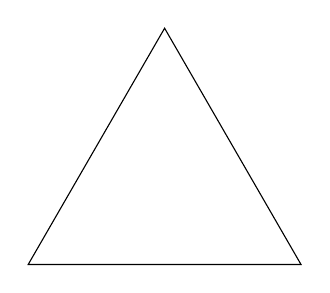
\begin{tikzpicture}
      \node[regular polygon, draw,
        regular polygon sides = 3,
        minimum size = 4cm] (p) at (0,0) {};
    \end{tikzpicture}
  \end{center}

  To keep track of what's going on, put names on your vertices.

  There are only 6 possible symmetries of this group. Symmetries are determined
  by where the labels on the vertices go.
}

Consider an $n$-gon and take $A_1$, any vertex of this $n$-gon. You can take
$A_1$ to any of $n$ vertices, then chose whether to put $A_2$ (a neighbor of
$A_1$) clockwise or counter-clockwise of $A_1$. Then, everything else is determined!

\note {
  $D_{2n}$ is {\bf not} Abelian. Simply convince yourself that rotate then
  reflect is {\it different} from reflect, then rotate. If you're not convinced,
  draw it!
}

\example {
  In $D_{2n}$, if $x$ is a reflection, $y$ is not counter-clockwise by $2 \pi /
  n$ radians
}

{\bf Fact}: $D_{2n} \le S_n$ for $n \ge 3$. Since symmetry in $D_{2n}$ is a
permutation of vertex labels.

{\bf Exercise}: Show that $D_6 \cong S_3$.

\definition {
  If $H \le G$, define

  \[
    aH = \{ ah \mid h \in H \} \subseteq G
  \]

  is called a {\bf left coset} of $H$, with $a \in G$ fixed.
}

{\bf Proposition}: If we have a homomorphism $\phi: G \to G'$, and $a, b \in G$,
then if $K = \ker(\phi)$ (which remember is a subgroup of $G$), then

\[
  \phi(a) = \phi(b) \Leftrightarrow a^{-1}b \in K \Leftrightarrow b \in a K
  \Leftrightarrow a K = b K
\]

What we have is that cosets determine when elements map to the same spot under a
homomorphism.

{\bf Proof}:

$\phi(a) = \phi(b) \Leftrightarrow \phi(a)^{-1}\phi(b) = e \Leftrightarrow
\phi(a^{-1}b) = e \Leftrightarrow a^{-1}b \in K \Leftrightarrow a^{-1}b = k$ for
some $k \in K$, which is true if and only if $b = ak$ for some $k \in K$, again
if and only if $b \in a K$

\begin{align*}
  &\phi(a) = \phi(b) \\
  \Leftrightarrow &\phi(a)^{-1}\phi(b) = e \\
  \Leftrightarrow &\phi(a^{-1}b) = e \\
  \Leftrightarrow &a^{-1}b \in K \\
  \Leftrightarrow &a^{-1}b = k \\
  \Leftrightarrow &ab = k
\end{align*}

\TODO {}

Similarly, $a \in bK$.

\example {
  $a \in bk$ and $b \in ak$ if and only if $aK = bK$.
}

In fact, for any subgroup $H \le G$, $a^{-1}b \in H \Leftrightarrow b \in aH
\Leftrightarrow aH = bH$.

So given $H \le G$, define a relation $\sim$ no $G$ by $a \sim b \Leftrightarrow
a \in bH$. But by the above, this true if and only if $aH \Leftrightarrow bH$.
Hence $\sim$ is an equivalence relation.

What we get out of this is that

\begin{enumerate}
  \item {\bf the cosets of $H$ partition $G$}.
  \item The number of cosets of $H$ is the index of $H \in G$, written $[G : H]$, which may be $\infty$.
\end{enumerate}

\QUESTION {} How do we compute $[G : H]$?

\date{Mon 12 Feb 2024}

\note {
  \begin{itemize}
    \item Homework 3 is due Thursday this week
    \item Midterm 1 is two Fridays from today.

      Exam content will be up until Monday, and there will be a review on
      Wednesday.
  \end{itemize}
}

\section{Cosets}

{\bf Recall}: If $H \le G$, and $a \in G$, the {\it left coset} $aH = \{ah \mid
h \in H \}$.

Last time we saw that $a \in bH$ if and only if $b \in aH$, if and only if $aH =
bH$, which gives us this equivalence relation $a \sim b \Leftrightarrow a \in
bH$, which means we get a partition on the set $G$ of this group, and it's
partitioned on the cosets! So the cosets of $H$ partition $G$.

{\bf Lemma}: The size of any coset is the same as the original size of the
subgroup for any element $a \in G$. In other words, all cosets are the same
size!

{\bf Proof}: We can write a map $f: H \to aH$ where $h \mapsto ah$.

Let's prove that this is bijective.

\begin{itemize}
  \item {\bf Injective}: If $f(h) = f(h')$, then $ah = ah'$, but then because
    this is a group, we can multiply by $a^{-1}$ on both sides and so $h = h'$.

  \item {\bf Surjective}: Given $ah \in aH$, then $f(h) = ah$.
\end{itemize}

So $f$ is a bijection, so $|H| = |aH|$.

\note {
  We only care about this when our sets are finite! In that case, injectivity
  and surjectivity are the same {\bf as long as the domain and codomain are the same
  size!}
}

We finally get to one of the landmars of Group Theory, this is


\section{Lagrange's Theorem}
\Theorem {
  If $H \le G$ and $G$ is finite, then $|H|$ divides $|G|$.
}
{
  The cosets of $H$ partition $G$, and all have the same size. Therefore

  \[
    |G| = \sum_{aH} |aH| = \sum_{[G : H]} = |H| [G : H]
  \]

  Where $aH$ is a left coset of $G$.

  Furthermore, $|H|$ divides $|G|$ and $[G : H] = \frac{|G|}{|H|}$
}

\Corollary {
  If $a \in G$, then $|a|$ divides $|G|$
}
{
  $|a| = |\lr {a}|$ and $\lr {a} \le G$ so we are done by Lagrange's Theorem.
}

\note {
  {\bf The converse is not necessarily true!}
}

\Corollary {
  If $|G| = p$ a prime, then $G$ is cyclic.
}
{
  Take $a \in G$, $a \ne e$, then $|a| \ne 1$ (because its not the identity.)
  But $|a| \mid p$, so in fact $|a| = p$. But $|G| = p$ and $\lr {a} \le G$, and
  $\lr {a} = G$, so $G$ is cyclic.

  In fact, every element in $G$ which is not the identity is a generator of the
  group!
}

\Lemma {
  If $G, G'$ are cyclic groups of order $n$, then $G \cong G'$.
}
{
  We saw that $G \cong \Z_n$, and $G' \cong \Z_n$, and so it follows that $G
  \cong G'$.
}

\Corollary {
  All order $p$ groups, $p$ a prime, are isomorphic.
}
{
  Proof Omitted. It just follows from everything we've seen so far!

  {\bf Up to isomorphism}, there is only one group of order $p$.
}

Let's go back and talk about those left cosets.

{\bf Remark}. We can also define {\bf right cosets}

\[
  Ha = \{ ha \mid h \in H \}
\]

And in fact, everything we proved so far could have worked with right cosets
too!

{\it A priori}, the partitions generated by a left and right coset might be
different.

\definition {
  A subgroup $H \le G$ is a {\bf normal subgroup} if

  \[
    aH = Ha
  \]

  for all $a \in G$. We write $H \trianglelefteq G$.
}

If $\phi: G \to G'$ is a homomorphism, then $K = \ker(\phi)$ is normal. The
claim here is that kernels are normal subgroups.

{\bf Proof}:

Given $a \in G$, $aK = \phi^{-1}(\phi(a)) = \{b \in G \mid \phi(b) =
\phi(a)\}$. Since the inverse function might not exist, we're just looking for
the {\it pre-image} here (Recall the proposition from last week.)

\note {
  We could have redone this proposition with right cosets!

  \[
    aK = Ka
  \]
}

We have lots of normal subgroups because we have lots of Homomorphisms.

\example {
  \begin{itemize}
    \item $\sgn : S_n \to (\{\pm 1\}, \times)$ with

      \[
        \sigma \mapsto \begin{cases}
          1 & \sigma \text{ even} \\
          -1 & \sigma \text{ odd}
        \end{cases}
      \]

    \item $\ker(\sgn) = An$ implies $An \trianglelefteq S_n$.
  \end{itemize}
}

An alternative way to prove that $H \trianglelefteq G$:

$aH = Ha$ if and only if $aHa^{-1} = H$.

\note {
  Warning:

  \begin{itemize}
    \item If $ah \in aH = Ha$, it's {\bf not necessarily the case} that $ah = ha$.

      Remember, the sets are equal, but not necessarily the elements! Instead, $ah =
      h'a$ for some $h' \in H$.

    \item Similarly, $aha^{-1} = h^{-1}$, not necessarily $h$.
  \end{itemize}
}

Normal subgroups are perfectly designed for doing algebra with cosets! $H
\trianglelefteq G$, then

\[
  (aH)(bH) = \{(ah)(bh') \mid h, h' \in H \}
\]

What is this set?, Well

\begin{align*}
  (aH)(bH) &= \{(ah)(bh') \mid h, h' \in H \} \\
           &= \{a \underbrace{(hb)}_{\in Hb = bH} h' \mid h, h' \in H \} \\
           &= \{a (b h'') h' \mid h', h'' \in H \} \\
           &= \{(ab)(h'' h') \mid h', h'' \in H \}
\end{align*}

As $h'$ and $h''$ range over $H$, we get all elements of $H$. So this set is
$(ab)$ times all elements of $H$, so we have

\[
  (aH)(bH) = (ah) H
\]

Alternatively, we may write

\begin{align*}
  aH bH &= a(Hb)H = a(bH)H \\
        &= ab (HH) = abH
\end{align*}

With these cosets, we can form new groups! This multiplication of cosets is a
binary operation on the set of cosets.

In order to simplify notation, let $\bar a = a H$, and we let

\[
  G / H = \{aH \mid a \in G\} = \{\bar a \mid a \in G \}
\]

With binary operation $\bar a \cdot \bar b = \overline{ab}$

{\bf Claim}: $G / H$ is a group, and furthermore, $\pi: G \to G / H$ where $a
\mapsto \bar a$, is a group homomorphism, with $\ker(\pi) = H$.

\definition {
  $G / H$ is called the {\bf quotient group} of $G$ by $H$.
}

{\bf Proof of Claim}:

\begin{itemize}
  \item {\bf Proof of Group}

    \begin{itemize}
      \item {\bf Associativity}: $(\bar a \cdot \bar b) \cdot \bar c = \overline
        {ab} \cdot \bar c = \overline{(ab)c}$. Since $G$ is associative,
        $\overline{(ab)c} = \overline{a(bc)}$ and furthermore, $\bar a \cdot
        \overline{bc} = \bar a (\bar b \cdot \bar c)$.

      \item {\bf Identity}: $\bar e = eH = H$ is the identity.
      \item {\bf Inverses}: $\overline{a^{-1}} \cdot \overline{a} =
        \overline{a^{-1} a} = \overline{e}$. So $\overline{a}^{-1} =
        \overline{a^{-1}}$.
    \end{itemize}

  \item {\bf Group Homomorphism}: $\pi(ab) = \overline{ab} = \bar a \cdot \bar b
    = \pi(a) \pi(b)$

  \item {\bf Kernel}: $\pi(a) = \bar e$ if and only if $aH = eH = H$, if and
    only if $a \in eH = H$. So $H = \ker(\pi)$
\end{itemize}

\date {Wed 14 Feb 2024}

\note {
  Recall: the Exam is next Friday, there are 2 practice Midterms. Not
  necessarily from this class, but they are the right material.

  Also on there is Exam 1 material not on homework. Homework style questions on
  material that we didn't have a Homework on. Quotient Groups, First Isomorphism
  Theorem, ...
}

We are talking about normal subgroups and quotient groups. Let's talk about
normal subgroups some more before getting into examples.

We saw that a subgroup is normal if $aH = Ha$ for all $a \in G$, $H \le G$.

{\bf Claim}: $H$ is normal if and only if $aHa^{-1} = H$ for all $a \in G$.
Why is this the same thing?

{\bf Proof}

$\Rightarrow$

Assume $H$ is normal. Let $a \in G$, then we know that $aH = Ha$ (that's what it
means to be normal.) If we want to show that $aHa^{-1} = H$, we must show that
these two sets are subsets of each other.

If $aha^{-a} \in aHa^{-1}$, then $ah \in aH$, but since $aH = Ha$, there exists
some $h'$ with $ah = h'a$. Hence $aha^{-a} = h'aa^{-1} = h' \in H$. So $aHa^{-1}
\subseteq H$. We wanna prove the other direction now.

If $h \in H$, we want to show that $h \in aHa^{-1}$. We know that $h =
haa^{-1}$, but $ha = ah'$ for some $h'$, so $haa^{-1} = ah'a^{-1}$, so $H
\subseteq aHa^{-1}$.

So $H = aHa^{-1}$.

$\Leftarrow$

Assume $aHa^{-1} = H$ for all $a \in G$. We want to show that $aH = Ha$, let $ah
\in aH$, we know that $aha^{-1} \in H$, which means that there exist some
element of $H$ with $aha^{-1} = h'$, and so $ah = h'a \in Ha$. So $aH \subseteq
Ha$.

The other direction works in the exact same way.

--

\example {
  If $K = \ker(\phi: G \to G')$, then $K \trianglelefteq G$, because if
  $aka^{-1} \in aKa^{-1}$, then

  \[
    \phi(aka^{-1}) = \phi(a) \phi(k) \phi(a)^{-1} = e
  \]

  So $aka^{-1} \in K$, so $aKa^{-1} \le K$.

  In fact, $aKa^{-1}$ is the same size as $K$ is conjugation does not change the
  size, so $aKa^{-1} = K$.
}

Now let's talk about quotient groups.

Let $G = S_n$ and $H = A_n$. We saw last time that $A_n \trianglelefteq S_n$
since $A_n = \ker(\sgn)$. Let's check this explicitly.

Given a permutation $\sigma \in A_n$ and $\tau \in S_n$. We want to show that
$\tau \sigma \tau^{-1} \in A_n$.

Well, $\sigma$ is even. If $\tau$ is odd, then so is $\tau^{-1}$ so $\tau
\sigma \tau^{-1}$ is even. If $\tau$ is even, then so is $\tau^{-1}$, so again
$\tau \sigma \tau^{-1}$, so $\tau \sigma \tau^{-1} \in A_n$.

\sidenote {
  Why is it that $|\sigma| = |\sigma^{-1}|$, with $\sigma \in S_n$? Well, just
  think of

  \[
    \sigma = (a_1 a_2)(a_2 a_3) \cdots (a_{k  - 1} a_k)
  \]

  Then

  \[
    \sigma^{-1} = (a_{k - 1} a_k) \cdots (a_2 a_3)(a_1 a_2)
  \]

  so $|\sigma| = |\sigma^{-1}|$.
}

So $\tau \sigma \tau^{-1} \in A_n$, and $A_n$ is normal.

\section{Quotient Groups}

Assume that $H \trianglelefteq G$. Last time, we defined that

\[
  G / H = \{aH \mid a \in G\} = \{\bar a \mid a \in G \}
\]

With the binary operation $\bar a \cdot \bar b = \overline{ab}$.

\example {
  If $G = S_n$ and $H = A_n$. Since $|S_n| = n!$, $|A_n| = n! / 2$. We know that

  \[
    [S_n : A_n] = \frac{n!}{n! / 2} = 2
  \]

  and so $|S_n / A_n| = 2$ and thus $S_n / A_n \cong \Z_2$. \QUESTION{} Why is this
  isomorphic?
}

{\bf Remark}: ``Identify the quotient group" means ``Find a familiar group to
which the quotient group is isomorphic."

\example {
  Identify $S_n / A_n$. The answer is $S_n / A_n \cong \Z_2$
}

{\bf $S_n / A_n$ in more detail.}

The cosets of $A_n$ are: either

\begin{itemize}
  \item $A_n$ (the coset of even permutations)
  \item $(12)A_n$ (the coset of odd permutations)
\end{itemize}

So $S_n / A_n = \{ \bar e, \overline{(12)} \}$

\TODO{} see multiplication table.

This is clearly isomorphic to $\Z_2$, where we just send $\bar e \to \bar 0$ and
$\overline{(12)} \to \bar 1$.

\example {
  Consider $G = \Z_n$, $H = \lr{\bar m}$ for $\bar m \in \Z_n$.

  {\bf Fact}: Any subgroup of an Abelian group is normal. This should make
  sense, because left and right cosets only different by the order in which you
  write, which doesn't matter for Abelian groups!

  Say that $\gcd(m, n) = d$, then $|\bar m| = \frac{n}{d}$. Take $[G : H] = |G /
  H|$, and we know by Lagrange's theorem that $|G / H| = |G| / |H| = n / (n / d)
  = d$.

  On Homework 2, we showed that if $\phi: G \to G'$ is onto and $G$ is cyclic,
  then $G'$ is cyclic.

  Here, we have the onto homomorphism $\pi: G \to G / H$. Since $G$ is cyclic,
  so is $G / H$, which means $G / H$ is a cyclic group of order $d$, hence $G /
  H \cong \Z_d$.
}

Alternatively: Assume that $\bar m$ is the smallest element in $H$ (i.e. $\bar m
= \bar d$.)

What are the cosets?

The cosets of $H$ are

$\{\bar 0 + H, \bar 1 + H, \dots, \overline{d - 1} + H\}$, and $\bar a + H = H
\Leftrightarrow \bar a \in H$, since $aH = eH \Leftrightarrow a \in eH = H$.

We can already see that $G / H$ is cyclic, generated by $\bar 1 + H$. Hence $G /
H \cong \Z_d$, where $\phi(\bar k + H) = \bar k$.

Our goal is to prove the 1st Isomorphism Theorem.

\example {
  Take $\sgn: S_n \to \Z_2$, but this time with

  \[
    \sigma \to \begin{cases}
      \bar 0 & \sigma \text{ even} \\
      \bar 1 & \sigma \text{ odd} \\
    \end{cases}
  \]

  $\sgn$ is onto, so $\image = \Z_2$. $\ker(\sgn) = A_n$, then $S_n / A_n \cong
  \Z_2$.
}

\example {
  $\phi: \Z \to \Z_n$ with $k \to \bar k$.

  $\phi$ is onto, $\ker \phi = n \Z$, then $\Z / n\Z \cong \Z_n$
}

\date{Fri. 16 Feb 2024}

Let's look at some examples of homs

\example {
  Consider $\det: \gl_n(\R) \to (\R \setminus \{0\}, \times)$. We know that
  $\ker(\det) = \{ A \in \gl_s(\R) \mid \det(A) = 1 \} = \sl_n(\R)$, and we now
  see that this is a normal subgroup.

  $\sl_n(\R) \trianglelefteq \gl_n(\R)$, as given any $A \in \sl_n(\R)$, $B \in
  \gl_n(\R)$, $BAB^{-1}$ has $\det = 1$, so $BAB^{-1} \in \sl_n(\R)$, so
  $\sl_n(\R)$ is normal.
}

Because both of these groups are infinite, and so is the index, we can't just
cheat like last time and take a look at what this is isomorphic to. We also know
that $\det$ is surjective, but the 1st isomorphism theorem tells us that
$\gl_n(\R) / \sl_n(\R) \cong \R \setminus \{0\}$.

One more example before the proof.

\example {
  Consider $\varphi: \C \setminus \{0\} \to \R \setminus \{0\}$ with $\varphi(z)
  = |z|$, the map which takes a complex number to its modulus (its length.)

  {\bf Fact}: $|zw| = |z| |w|$, so $\varphi$ is a homomorphism.

  Notice that that the image of $\varphi$ is only positive numbers, and
  $\ker(\varphi)$ is all the complex numbers with modulus $1$ (or length 1.)
  This is all complex numbers of the form $a + bi = 1$, so $a^2 + b^2 = 1$,
  which is the unit circle!

  Here, our 1st isomorphism theorem tells us that $\C \setminus \{0\} /
  \text{unit circle} \cong \R_{\ge 0}$.

  Think about this:

  \[
    \C \setminus \{0\} = \{re^{i \theta} \mid r \in \R_{\ge -0}, e^{i\theta} \in
    \text{ unit circle}\}
  \]

  What we're left with is just the module information.
}

{\bf Question}: Can you quotient out by the real numbers? Well remember that
complex numbers under multiplication is Abelian, so every subgroup is normal,
which means that you can! Do you get something isomorphic to the unit circle?
Think about it!

Ok! Time for the theorem.

\section{1st Isomorphism Theorem}

Given a homomorphism $\varphi: G \to G'$, we have that

\[
  G / \ker(\varphi) \cong \image(\varphi)
\]

{\bf Proof}

We have a hom $\varphi: G \to G'$. Let's assume that it's onto. If it's not,
replace $G'$ to $\image(\varphi)$ (Basically, we just change the codomain to
make it onto.)

Let $K = \ker(\varphi)$, and we want to show that $G / K \cong G'$. Let $\pi:
G \to G / K$ (since $K$ is normal, we can do this!) This is the map $\pi(a) =
\bar a$.

We define $\bar \varphi: G / K \to G'$, which takes $\bar \varphi(\bar a) =
\varphi(a)$


Here's a picture.

% https://q.uiver.app/#q=WzAsMyxbMCwwLCJHIl0sWzIsMCwiRyciXSxbMSwxLCJHL0siXSxbMCwxLCJcXHZhcnBoaSJdLFswLDIsIlxccGkiLDJdLFsyLDEsIlxcYmFyIFxcdmFycGhpIiwyXV0=
\begin{center}
  \begin{tikzcd}
    G && {G'} \\
    & {G/K}
    \arrow["\varphi", from=1-1, to=1-3]
    \arrow["\pi"', from=1-1, to=2-2]
    \arrow["{\bar \varphi}"', from=2-2, to=1-3]
  \end{tikzcd}
\end{center}


We check that $\bar \varphi$ is well-defined, i.e. if $\bar a = \bar b$, check
that $\bar \varphi(\bar a) = \bar \varphi(\bar b)$

\begin{align*}
  \bar a = \bar b &\Leftrightarrow aK = bK \\
                  &\Leftrightarrow \varphi(a) = \varphi(b) \\
                  &\Leftrightarrow \bar \varphi(\bar a) = \bar \varphi(\bar b)
\end{align*}

So $\bar \varphi$ is a function.

{\bf Claim}: $\bar \varphi$ is an isomorphism.

\begin{itemize}
  \item {\bf Homomorphism}:

    $\bar \varphi(\bar a \cdot \bar b) = \bar \varphi(\overline{ab}) =
    \varphi(ab) = \varphi(a) \varphi(b) = \bar \varphi(\bar a) \bar
    \varphi(\bar b)$.

  \item {\bf One to one}:

    We'll show that $\ker(\bar \varphi) = \{ \bar e \}$ (usefull trick btw, if you have a hom, you only need to check this)

    if $\bar \varphi(\bar a) = e$, then $\varphi(a) = e$, but then $a \in
    \ker(\varphi) = K$, so $\bar a = aK = K = \bar e$.

  \item {\bf Onto}:

    if $b \in G'$, then there exists $a \in G$ with $\varphi(a) = b$
    (remember, since we assumed $\varphi$ to be onto!)

    So we get $\bar \varphi(\bar a) = \varphi(a) = b$.
\end{itemize}

Hence $\bar \varphi: G / K \to G'$ is an isomorphism, which concludes the
proof.


\note {
  For the exam, don't worry about being able to prove, this. You should be able
  to {\it use} these techniques. You should be able to use the tools and
  techniques from class.

  The techniques that go into proofs are good to understand though!
}

\TODO{} draw tetrahedron with colors. Oh god

Let $G$ be the group of symmetries of the regular tetrahedron. Symmetry is
determined by what it does to vertices. All permutations of vertices are
possible since all vertices are neighbors. Immediately, we see that

\[
  G \cong S_4
\]

Every symmetry also permutes the colors of the edges.

\[
  \{\text{red}, \text{green}, \text{blue}\}
\]

The group of permutations of this set is isomorphic to $S_3$ of course! Because
we have 3 things in it.

So we get a map $\varphi: S_4 \to S_3$ which takes $\sigma$, a symmetry of the
tetrahedron, to the number of ways to permute the $3$ colors.

We're not going to prove that $\varphi$ is a homomorphism.

Let $C_1 = \text{green}, C_2 = \text{blue}, C_3 = \text{red}$. Then $(12) \in
S_4$ is a reflection of the tetrahedron.

\TODO{} draw this somehow

Another way to think about is is that vertices $3$ and $4$ don't move, but $1$
and $2$ switch.

So $\varphi((12)) = (C_1 C_2)(C_3) \in S_3$. It swaps green and blue and keeps
red fixed.

{\bf Exercise 1}: $\varphi$ is surjective. Every way of permuting the colors is
possible.

{\bf Exercise 2}: $\ker(\varphi) = \{e, (12)(34), (13)(24), (14)(23) \}$. This
is the Klein-4 group!!! Also known as $K_4$.

This is a group of order $4$ which is {\bf not} isomorphic to $\Z_4$, since all
elements of $K_4$ are order $1$ or $2$.

Here, the 1st isomorphism theorem tells us that $S_4 / K_4 \cong S_3$.

{\bf Warning}: $K_4$ and $\Z_4$ are Abelian groups of order $4$. Both have
normal subgroups of order $2$. If $K_4 = \{e, a, b, ab\}$, $H = \{e, a\}$ and
$\{\bar 0, \bar 2\} \le \Z_4$, and $K_4 / H \cong \Z_2$, $H \cong \Z_2$, and
$\Z_4 / H \cong \Z_2$.

Why is this a warning? Because we {\bf cannot} reconstruct the original group
from $H$ and $G / H$.

\note {
  We'll do product groups on Monday, which is testable. The rest will not be.
}

\date{Mon. 19 Feb 2024}

Today we are talking about Product Groups!

\section{Product Groups}

Today we try to build up larger groups from smaller groups.

Let's write out explicitly the binary operations. Let $(G, p), (G', p')$ be two
groups.

The set

\[
  G \times G' = \{(g, g') \mid g \in G, g' \in G' \}
\]

Can be given a binary operation

\[
  (g, g') \cdot (h, h') = (p(g, h), p'(g', h'))
\]

Basically, you do the operations component-wise.

{\bf Claim}: This is a group!

\begin{enumerate}
  \item {\bf Identity}: $(e_G, e_{G'})$
  \item {\bf Inverses}: $(g, g')^{-1} = (g^{-1}, (g')^{-1})$
\end{enumerate}

\definition {
  $G \times G'$ is the {\bf product} of $G$ and $G'$. It's also known as the
  {\bf direct product}.
}

\note {
  $|G \times G'| = |G| \cdot |G'|$
}

From this we can get special Homomorphisms. Quite a few in fact.

% https://q.uiver.app/#q=WzAsNSxbMiwxLCJHIFxcdGltZXMgRyciXSxbNCwwLCJHIl0sWzQsMiwiRyciXSxbMCwwLCJHIl0sWzAsMiwiRyciXSxbMCwxLCJcXHBpX0ciXSxbMCwyLCJcXHBpX3tHJ30iLDJdLFszLDAsIlxcaW90YV97R30iLDJdLFs0LDAsIlxcaW90YV97Ryd9IiwyXV0=
\begin{center}
  \begin{tikzcd}
    G &&&& G \\
    && {G \times G'} \\
    {G'} &&&& {G'}
    \arrow["{\pi_G}", from=2-3, to=1-5]
    \arrow["{\pi_{G'}}"', from=2-3, to=3-5]
    \arrow["{\iota_{G}}"', from=1-1, to=2-3]
    \arrow["{\iota_{G'}}"', from=3-1, to=2-3]
  \end{tikzcd}
\end{center}

All of these are homomorphisms. We say that $\iota_G$ and $\iota_{G'}$ are {\bf
inclusions}, and that $\pi_G$ and $\pi_{G'}$ are {\bf projections}. Let's look
at them in more detail

{\bf Inclusions}
\begin{itemize}
  \item $\iota_G(g) = (g, e)$. We have no other choice here for the second
    element. Think about why.
  \item $\iota_{G'}(g') = (e, g')$
\end{itemize}

{\bf Projections}
\begin{itemize}
  \item $\pi_G(g, g') = g$
  \item $\pi_{G'}(g') = g'$
\end{itemize}

Note that these maps are onto, and in fact $\ker(\pi_G) = \{ (e_{G}, g') \mid g'
\in G' \}$. Similarly, $\ker(\pi_{G'}) = \image(\iota_G)$.

Now using the 1st isomorphism theorem, we know that $G \times G' / G' \cong G$.
This means that $\iota_{G'}(G') \le G \times G'$.

Similarly, $G \times G' / G \cong G$, meaning that $\iota_G(G) \le G \times G'$.

This is fairly inline with how we expect the quotient group to behave.

Let's look at an

\example {
  \[
    \Z_2 \times \Z_3 = \{ (\bar 0, \bar 0), (\bar 1, \bar 0), (\bar 0, \bar 1),
    (\bar 0, \bar 2), (\bar 1, \bar 2) \}
  \]
}

Let's turn our attention to $\lr { (\bar 1, \bar 1) }$. We have that

\[
  \lr { (\bar 1, \bar 1) } = \{ (\bar 0, \bar 0), (\bar 1, \bar 1), (\bar 0, \bar
  2), (\bar 1, \bar 0), (\bar 0, \bar 1), (\bar 1, \bar 2) \}
\]

So in fact $(\bar 1, \bar 1)$ is a generator of $\Z_2 \times \Z_3$. This means
that $\Z_2 \times \Z_6$ is not a new group, it's isomorphic to $\Z_6$ ! In fact,
this is generalizable.

{\bf Proposition}

$\Z_m \times \Z_n \cong \Z_{mn}$ if and only if $\gcd(m, n) = 1$.

{\bf Proof}

All we have to do is figure out when the group on the left is cyclic.

{\bf Lemma}:

The order of $(g, g') \in G \times G'$ is the $\lcm(|g|, |g'|)$.

{\bf Proof of Lemma}

If $\gcd(m, n) = 1$, then the $\lcm(|\bar 1|, |\bar 1|) = \lcm(m, n)$. Moreover,

\[
  \lcm(m, n) = \frac{mn}{\gcd(m, n)}
\]

This means that $(\bar 1, \bar 1)$ generates $\Z_m \times \Z_n$, so it is
cyclic, and so it is isomorphic to $\Z_{mn}$

On the other hand, if $\gcd(m, n) \ne 1$, then for any $(\bar a, \bar b) \in
\Z_m \times \Z_n$, then $|(\bar a, \bar b)| = \lcm(|\bar a|, |\bar b|) \le
\lcm(m, n) < mn$, in which case $\Z_m \times \Z_n$ cannot be cyclic! And so it
is {\bf not} isomorphic to $\Z_{mn}$

For instance, $\Z_2 \times \Z_2 \not\cong \Z_4$.

{\bf Proposition}: There are two groups of order $4$, up to isomorphism.

\[
  \Z_4 \text{ or } \Z_2 \times \Z_2
\]

{\bf Proof}: Let $G$ be a group of order $4$. If $G$ is cyclic, then $G \cong
\Z_4$. If not, then $|a| = 2$ for all non-trivial elements in our group. Pick $a
\in G$, and $b \in G$ with $b \ne e$ and $b \ne a$. Then

\[
  ab \ne \begin{cases}
    e & \text{ as } b \ne a^{-1} = a \\
    a & \text{ as } b \ne e \\
    b & \text{ as } a \ne e
  \end{cases}
\]

So $ab$ is the $4$ element of $G$, and thus $G = \{e, a, b, ab\}$. Then we have
that $\varphi: \Z_2 \times \Z_2 \to G$ with

\begin{itemize}
  \item $(\bar 0, \bar 0) \mapsto e$
  \item $(\bar 1, \bar 0) \mapsto a$
  \item $(\bar 0, \bar 1) \mapsto b$
  \item $(\bar 1, \bar 1) \mapsto ab$
\end{itemize}

Is an isomorphism.

{\bf Structure Theorem for Finitely Generated Abelian Groups}

If $G$ is finitely generated, (i.e. there is a finite set $S \subseteq G$ such
that all elements of $G$ are products of elements of $S$ and their inverses) and
$G$ is Abelian, then

\[
  G \cong \Z \times \cdots \times \Z \times \Z_{m_1} \times \cdots \times \Z_{m_k}
\]

Moreover, if $G$ is finite and Abelian, then

\[
  G \cong \Z_{m_1} \times \cdots \times \Z_{m_k}
\]

\btw {
  This is all the material you need to know for this Exam. From this point
  forward is {\bf not} exam material.
}

\section{Semidirect Product}

Given a group $G$, the set $\Aut(G)$ of {\bf automorphisms} of $G$ (i.e.
isomorphisms $G \to G$) is a group under composition.

\definition {
  Let $G, H$ be groups, $\varphi: H \to \Aut(G)$ be a homomorphism with
  $\varphi(h) = \varphi_h$. Then the group

  \[
    G \times_\varphi H \text{ or } G \rtimes H
  \]

  is called a {\bf semidirect product}, where the elements $(g, h) \in G \times
  H$, but the binary operation

  \[
    (g, h)(g', h') = (g \cdot (\varphi_h(g')), hh')
  \]
}

The set is the same! But the binary operation is different, so we have a new
group structure.

The identity: $(g, h)(e, e) = (g \varphi_h(e), he) = (ge, he) = (g, h)$.
On the other side: $(e, e)(g, h) = (e \varphi_e(g), eh) = (eg, eh) = (g, h)$,
since $\varphi_e = \varphi(e) = e_{\Aut(G)}$ so $\varphi_e(g) = g$.

\example {
  If $\varphi: H \to \Aut(G)$ is the identity, then

  \[
    (g, h)(g', h') = (g \varphi_h(g'), hh') = (gg', hh')
  \]

  So

  \[
    G \times_\varphi H = G \times H
  \]
}

\example {
  Let $G = \Z_n$ and $H = \Z_2$ with $\varphi: \Z_2 \to \Aut(\Z_n)$ with $\bar 0
  \mapsto e$ and $\bar 1 \mapsto f$. $f: \Z_n \to \Z_n$ is determined by $f(\bar
  1)$.

  We need $f \circ f = id$ as $\varphi(\bar 1 + \bar 1) = \varphi(\bar 0) = id$.
  For any $n$, $f = id$ or $f(\bar 1) = \overline{-1} = \overline{(n - 1)}$.

  With the former, $\Z_n \times_\varphi Z_2 \cong \Z_n \times \Z_2$. With the
  latter, $\Z_n \times_\varphi \Z_2 \cong D_{2n}$.
}

\date{Wed. 21 Feb 2024}

Today is review!

Structure of the Exam:
\begin{itemize}
  \item 4 Questions
  \item First question is short answer. Similar to the 2019 Midterm
  \item 3 Longer questions, similar to the 2019 midterm.
\end{itemize}

{\bf Exam Questions}

\section{Exam 1 Review}

\subsection{Common Groups and their properties}

Useful for having a repertoire of questions.

\begin{itemize}
  \item $\Z$, $\Z_n$. This is {\bf always} under addition by default, {\bf even
    if $n$ is prime!} These are

    \begin{enumerate}
      \item Cyclic
      \item Abelian
      \item Sometimes infinite? Or order $n$
    \end{enumerate}

    \note {
      All subgroups of cyclic groups are cyclic.
    }

  \item $(\Z_n^\times, \times)$. This is the group of integers relatively prime
    to $n \mod n$ under $\times$. It is

    \begin{enumerate}
      \item Abelian
      \item Not necessarily cyclic, so the order is complicated.
      \item Does not include $\bar 0$.
    \end{enumerate}

  \item $S_n$. The Symmetric group. It is

    \begin{enumerate}
      \item Non-Abelian
      \item Not cyclic
      \item $|S_n| = n!$
    \end{enumerate}

    We have some nice isomorphisms

    \begin{enumerate}
      \item $S_3 \cong D_6$, where $D_6$ is the symmetries of a {\bf triangle}.
      \item $S_2 \cong \Z_2$
    \end{enumerate}

  \item $D_{2n}$. The dyhedral group. The symmetries of a regular $n$-gon. It is

    \begin{enumerate}
      \item Non-Abelian
      \item Not cyclic
      \item Order $2n$
    \end{enumerate}

    And we have that $D_{2n} \le S_n$, but we only have $D_6 \cong S_3$.

    We have a nice notation for this. We say that it is generated by $x$, a
    reflection, and $y$ a rotation.

    \[
      D_{2n} = \{e, x, y, \dots, y^{n - 1}, yx, \dots, y^{n-1}x\}
    \]

    And we have that $yx = y^{-1}x$.

  \item $A_n$. The alternating group. $A_n \le S_n$ with

    \begin{enumerate}
      \item $|A_n| = n! / 2$, subgroup of even permutations.
    \end{enumerate}

  \item $\R, \C$ (under addition), $\R \setminus \{0\}, \C \setminus \{0\}, \Q
    \setminus \{0\}$ (under multiplication)

    These are

    \begin{enumerate}
      \item Infinite
      \item Non-cyclic.
    \end{enumerate}

  \item $\gl_n(\R), \sl_n(\R)$. These are

    \begin{enumerate}
      \item Infinite
      \item Non-Abelian
    \end{enumerate}

    Where the binary operation is Matrix multiplication.

  \item Product Groups $G \times H$ with

    \begin{enumerate}
      \item $|G \times H| = |G| \cdot |H|$.
      \item $|(a, b)| = \lcm(|a|, |b|)$.
    \end{enumerate}

    These groups are Abelian if and only if both $G$ and $H$ are Abelian.

    We saw

    \begin{enumerate}
      \item $\Z_2 \times \Z_2 \not\cong \Z_4$, the Klein-4 Group.
    \end{enumerate}

    We also saw $\Z_m \times \Z_n \cong \Z_{mn}$
\end{itemize}

$Z_2$ Can be written a number of different ways.

\example {
  Groups of order $30$.

  We know that $30 = 3 \cdot 5 \cdot 2$.

  \begin{enumerate}
    \item If we want an Abelian group, we have no choice but to use $\Z_{30}$.
      \TODO{} why?

      What about $\Z_2 \times \Z_3 \times \Z_5$? Well that's isomorphic to
      $\Z_{30}$, since $2, 3$ are coprime, and $6, 5$ are also coprime.

    \item Non-Abelian: $D_{30}$, the symmetries of a regular $15$-gon, or
      $\Z_{3} \times D_{10}$, or $\Z_5 \times D_6$.

      Why are these 3 groups different? Why are they not isomorphic?

      The approach is to think about many different things. Usually the approach
      is to find a property that holds in one group that does not hold in the
      other.

      \begin{itemize}
        \item It could be size. If the sizes don't match, no chance that there
          can be an isomorphism.
        \item Abelian-ness
        \item One of them could be that a group has a normal subgroup of order
          $5$, and the other does not.
        \item This group has an element of order $15$, and the other does not.
      \end{itemize}

      All those things can be used to show that things are not isomorphic.

      In the example above, we know that $D_{30}$ has 15 elements of order 2,
      $D_{10}$ for sure has 5. The claim is that this is all of them. Simply
      notice that

      \[
        |(\bar a, g)| = \lcm(|\bar a|, |g|) = \begin{cases}
          \lcm(1, |g|) = |g| \\
          \lcm(3, |g|) = 3|g|
        \end{cases}
      \]

      The problem is that $3|g|$ is never equal to $2$, so it has to be $|g|$.

      \TODO{} finish. So they cannot be isomorphic.
  \end{enumerate}
}

\begin{itemize}
  \item $\Z_2 \cong (\{\bar 0, \bar 1\}, +) \cong (\{\pm 1\}, \times)$
\end{itemize}

{\bf 2018, 7b}

We have a group of order 40, we want to know all Abelian groups of order 40.

How many ways can we write 40 as a product of cyclic groups which are not
isomorphic?

We know that

\[
  40 = 2 \cdot 2 \cdot 2 \cdot 5
\]

Well, we have
\begin{enumerate}
  \item $\Z_2 \times \Z_2 \times \Z_2 \times \Z_5$
  \item $\Z_2 \times \Z_4 \times \Z_5 \cong \Z_{10} \times \Z_4 \cong \Z_2
    \times \Z_{20}$
  \item $\Z_8 \times Z_5 \cong \Z_{40}$
\end{enumerate}

Recall that we were asked for Abelian groups, so its just a product of cyclic
groups.

{\bf How do we show something is normal?}

There are several ways. Two big ones:

\begin{enumerate}
  \item {\bf By the definition}:

    Show that $aH = Ha$ are the same coset for all $a \in G$.

    If there's not many cosets, this isn't too bad.

  \item {\bf Show that $aHa^{-1} \in H$ for all $a \in G$, and for all $h \in H$}

    This implies that $aHa^{-1} = H$.

    In fact, it's sufficient to show the one direction for all elements. This is
    because we know that we have a bijection between a group and its
    conjugation.

  \item {\bf If $G$ is Abelian}

    Then all your subgroups are normal, so we're done!

    This one is less applicable, but useful!
\end{enumerate}

\example {
  {\bf 2019, number 4}

  If $G$ is a group and $Z(G) = \{a \in G \mid ab = ba \forall b \in G \}$ is
  the center of the group.

  We want to show that $Z(G) \trianglelefteq G$, in order words, that it's a
  normal subgroup.

  {\bf Proof}

  $e \in Z$, so $Z \ne \varnothing$

  {\bf Closure}: If $z, z' \in Z$, then for any $a \in G$, then $zz'a = zaz' =
  azz'$ so $zz' \in Z$. So $Z$ is closed.

  {\bf Inverses}: If $z \in Z$, $a \in G$, $az^{-1} = (za^{-1})^{-1} =
  (a^{-1}z)^{-1} = z^{-1}a$ so $z^{-1} \in Z$.

  {\bf WARNING}: If you aren't told it's a subgroup, you have to show that too!

  {\bf Normal}: To show that it's normal, if $z \in Z, a \in G$ then $aza^{-1} =
  aa^{-1}z = z \in Z$ so $Z \trianglelefteq G$.
}

{\bf What's an example of a Bijection that's not a Homomorphism?}

Here's one

\[
  \varphi: \Z_4 \to \Z_4
\]

where

\begin{itemize}
  \item $\bar 0 \mapsto \bar 1$
  \item $\bar 1 \mapsto \bar 2$
  \item $\bar 2 \mapsto \bar 3$
  \item $\bar 3 \mapsto \bar 0$
\end{itemize}

Here, the identity does not map to the identity. Also

\[
  \varphi(\bar 0 + \bar 1) = \varphi (\bar 1) = \varphi(\bar 2)
\]

But

\[
  \varphi(\bar 0) + \varphi(\bar 1) = \bar 1 + \bar 2 = \bar 3
\]

and $\bar 3 \ne \bar 2$.

{\bf 2018, question 2}

$\sigma = (137)(2465)$, and $\tau = (152)(3647)$, want to find $\sigma \tau^{-1}$

Well, $\tau^{-1} = (125)(3746)$

Then $\sigma \tau^{-1} = (1453)(67)$ \TODO{} Show

How do we write this in terms of transpositions? Well

\[
  = (14)(45)(53)(67)
\]

\date{Mon. 26 Feb 2024}

Two more weeks of Group Theory, then we talk about Rings and Fields.

\section{Group Operations}

We've seen two examples of groups that have to do with sets. $S_n$, and
$D_{2n}$. $S_n$ is a bijection from $\{1, \dots, n\}$ to itself, and $D_{2n}$
whose elements are special examples of bijections of the regular $n$-gon itself.

These are examples of group actions.

\definition {
  If $S$ is a set and $G$ is a group. We say that $G$ {\bf acts} on $S$ (notated
  as $G \acts S$) if there is a map $\alpha: G \times S \to S$ satisfying two
  properties.

  \begin{enumerate}
    \item $\alpha(e, s) = s$. On the identity, we just want our set back,
      unchanged.

    \item $\alpha(ab, s) = \alpha(a, \alpha(b, s))$. Basically the combination
      of both of these is the same as doing one after the other.
  \end{enumerate}

  We often write $\alpha_a(s)$ for $\alpha(a, s)$. Then $\alpha_a: S \to S$ for
  every $a \in G$.

  We can also write $a * s$ for $\alpha(a, s) = \alpha_a(s)$. In this case, our
  definition becomes

  \begin{enumerate}
    \item $e * s = s$ for all $s \in S$
    \item $(ab) * s = a * (b * s)$ for all $s \in S$ and for all $a, b \in G$.
  \end{enumerate}
}

Let's look at an example

\example {
  $S = \{1, 2, \dots, n\}, G = S_n$, then $\alpha(\sigma, i) = \sigma(i)$.

  Here, $\sigma$ is a bijection from $S$ to $S$.

  In our other notation, $\sigma * i = \sigma(i)$.
}

\example {
  $S$ is a regular $n$-gon. Let $G = D_{2n}$, then $a * s = a(s)$, so here,
  symmetry is a function from $S$ to $S$
}

\note {
  Group actions are just functions on the sets! Nothing crazy is happening
  here, we're just formalizing some natural ideas.
}

\example {
  $S = \R^n$, $G = \gl_n(\R)$ and $A * \bar v = A \bar v$ where $A \in
  \gl_n(\R)$, $\bar v \in \R^n$.
}

\example {
  if $G = \text{Mat}_n(\R)$, the set of all matrices under addition, then

  \[
    (A + B) * \bar v = (A + B)\bar v
  \]

  But also

  \[
    A * (B * \bar v) = A \bar v (B \bar v) = AB\bar v
  \]

  which are not equal, so this doesn't work.
}

\example {
  Let $S = G$ and $G = G$, any group $G$. Then what's the action? Well, it's
  just the group operation.

  \[
    a * s = as
  \]

  Left multiplication by our group element is a group action!
}

\note {
  It's worth noting that all these things are happening on the left! If you
  multiplied on the right, that would not be a group action!

  \[
    a * s = sa
  \]

  {\it Is not a group action! We only do left group actions in this class.}

  This is because of how we've set up function composition.

  \[
    (ab) * s = s(ab) \ne s (ba) = a * (sb) = a * (b * s)
  \]
}

\example {
  Let $G = \gl_n(\R)$, and let $S$ be the set of ordered bases for $\R^n$.
}

\definition {
  If $s \in S$, then the {\bf orbit} of $s$ is

  \[
    O_s = \{ a * s \mid a \in G \}
  \]

  It's all the images of $s$ from $G$, the set of all things that can happen to
  it. The collection of all those images is the orbit.
}

\example {
  If $S$ is the triangle, and $G$ is $D_6$, then if $s$ is a vertex, $O_s$ is
  {\it all} the vertices. If $s$ is the midpoint of a line segment of the
  triangle, then $O_s$ is the set of all such midpoints.

  In general, if $s$ is a point on the triangle, its orbit will be all the
  points that you can get to by taking that point, and either rotating the
  triangle or flipping it around.

  The orbit of the center is just itself.
}

\note {
  We always have that $s \in O_s$.
}

If $s' \in O_s$, then $s' = a * s$ for some $a \in G$. Then

\begin{align*}
  s = e * s &= (a^{-1}a) * s \\
            &= a^{-1} * (a * s) \\
            &= a^{-1} * s' \in O_{s'}
\end{align*}

If $s' \in O_s$, then $s \in O_{s'}$.

What we get here is an equivalence relation! $s \sim s'$ if $s \in O_{s'}$. What
we get out of this is that {\bf the orbits partition $S$.} It follows that if
$O_s \cap O_{s'} \ne \varnothing$, then $O_s = O_{s'}$.

\definition {
  A group action is called {\bf transitive} if there is only one orbit. In other
  words, $O_s = S$ for any $s \in S$.
}

\example {
  Let $O(n) \acts \R^n$ (where $O(n)$ is the orthogonal group. This is a
  subset of $\gl_n(\R)$ where the columns form an orthonormal basis.)

  $A * \bar v = A \bar v$ is {\bf not} transitive, as for $\bar v = \bar 0$, so
  $O_{\bar 0} = \{0\}$ (the only place that $0$ goes to under linear
  transformations is $0$.)

  In fact $||A \bar v|| = \bar v$ for any $\bar v$. So orbits of this group
  action are $n$ dimensional spheres centered at the origin!
}

\note {
  You will never get a transitive group action from a matrix group since the
  origin is alone.

  \TODO{} what????
}

\example {
  $S_n \acts \{1, \dots, n\}$ is transitive. If $s = 1$, then if $\sigma = (1
  k)$, then $\sigma * 1 = \sigma(1) = k$. So $k \in O_1$ for all $k = 1, \dots,
  n$. So $O_1 = \{1, \dots, n\}$.
}

\subsection{Stabilizers}

\definition {
  If $s \in S$, the {\bf stabilizer} of $s$ is

  \[
    \Stab(s) = G_s = \{a \in G \mid a * s = s\}
  \]

  It's all the group elements that don't do anything to $s$. They {\it
  stabilize} $s$.
}

To bring it back, we pick an element of a set $s$, and using this element, we
can look at its orbit: the set of places it will go under every possible group
action, or we can look at its stabilizer, the set of elements of $G$ that keep
it as it is.

\note {
  The Stabilizer is elements of $G$, but the orbit is elements of $S$.
}

{\bf Claim}: The stabilizer is a subgroup of $G$.

{\bf Check}:
\begin{enumerate}
  \item {\bf Closed}:

    If $a, b \in G_s$. Then

    \begin{align*}
      (ab) * s &= a * (b * s) \\
               &= a * s \\
               &= s
    \end{align*}

    so $ab \in G_s$.

  \item {\bf Inverses}:

    \begin{align*}
      s = e * s &= (a^{-1} a) * s \\
                &= a^{-1} * (a * s)
    \end{align*}

    If $a \in G_s$, then $a * s = s$, so $s = a^{-1} * s$ and so $a^{-1} \in G_s$
\end{enumerate}

Hence $G_s \le G$.

\example {
  If $S_n \acts \{1, \dots, n\}$, let $s = n$, then

  \[
    G_s = \{\sigma \in S_n \mid \sigma(n) = n\}
  \]

  This is all the permutations where $n$ does not appear in the cycle notation!
  This is all the permutations that use $1$ to $n - 1$.
}

\example {
  $\gl_n(\R) \acts \R^n$. If $\bar v = \bar 0$, then

  \[
    G_{\bar 0} = \{A \in \gl_n(\R) \mid A \bar 0 = \bar 0\} = \gl_n(\R)
  \]

  So the stabilizer can be the whole group.

  Note that if $\bar v \ne 0$, then $G_{\bar v} < \gl_n(\R)$.
}

\example{
  $\Isom(\R^n) \acts \R^n$, then $G_{\bar 0} \cong O(n)$.

  \TODO{} what?????
}

\date{Wed. 28 Feb 2024}

\note {
  Most questions on the homework are on actions. By the end of this class you
  should be able to do all questions up to 4.
}

{\bf Recall}: $G \acts S$ is a group action. Given $s \in S$, we have

\begin{enumerate}
  \item {\bf Orbit} $O_s = \{a * s \mid a \in G\} = \{s' \in S \mid s' = a * s\text{ for some } a \in G\} \subseteq S$
  \item {\bf Stabilizer} $\Stab(s) = G_s = \{a \in G \mid a * s = s \} \le G$.
\end{enumerate}

{\bf Proposition}:

If $G \acts S$ and $s \in S$. Then

\begin{enumerate}
  \item $a, b \in G$, then $a * s = b * s$ if and only if $a^{-1} b \in G_s$
  \item If $a * s = s'$, then $G_{s'} = a G_{s} a^{-1} = \{aga^{-1} \mid g \in
    G_s\}$ is the conjugate subgroup!

    So the stabilizers are related, they are conjugate subgroups.

    {\bf Corollary}: If $G$ is finite, and $a * s = s'$, then $|G_s| = |G_{s'}|$
    because conjugation is a bijection so they must have the same size.
\end{enumerate}

\note {
  Compare (a) to: If $\phi: G \to G'$ is a hom, $\phi(a) = \phi(b)$ if and only
  if $a^{-1} b \in \ker(\phi)$.
}

{\bf Proof of Proposition}.

\begin{enumerate}
  \item $a * s = b * s$ if and only if $a^{-1} (a * s) = a^{-1} * (b * s)$, if
    and

    \begin{align*}
      a * s = b * s &\Leftrightarrow a^{-1} (a * s) = a^{-1} * (b * s) \\
                    &\Leftrightarrow (a^{-1} a) * s = (a^{-1} b) * s \\
                    &\Leftrightarrow s = (a^{-1} b) * s \\
                    &\Leftrightarrow (a^{-1} b) \in G_s
    \end{align*}

  \item Let $a * s = s'$. (this implies that $s = a^{-1} * s'$)

    If $aga^{-1} \in a G_s a^{-1}$, then $(aga^{-1}) * s'$.

    \begin{align*}
      (aga^{-1}) * s' &= a * (g * (a^{-1} * a')) \\
                      &= a * (g * s) = a * s = s' &\text{since $g \in G_s$} \\
    \end{align*}

    So $aga^{-1} \in G_{s'}$. Hence $a G a^{-1} \subseteq G_{s'}$.

    Similarly, $(a^{-1}) G_{s'}(a^{-1})^{-1} \subseteq G_s$, since $a^{-1} *  s'
    = s$. Since conjugation is a bijection, can conjugate by $a$:

    \[
      a(a^{-1}) G_{s'}(a^{-1})^{-1}a^{-1} \subseteq a G_s a^{-1}
    \]

    So $G_{s'} \subseteq a G_s a^{-1}$.

    Hence $a G_s a^{-1} = G_{s'}$
\end{enumerate}

\section {Orbit Stabilizer Theorem}

If $G \acts S$ and $s \in S$, then there is a bijection $f: \{aG_s\} \to O_s$
with $aG_s \mapsto a * s$.

{\bf Proof}:

\begin{enumerate}
  \item {\bf $f$ is  well-defined}.

    If $aG_s = b G_s$, then $a^{-1} b \in G_s$. Which implies that $a * s = b *
    s$ by the Proposition. So if the input cosets are the same, then the output
    is consistent, and $f$ is well-defined.

  \item {\bf $f$ is injective}.

    If $f(aG_s) = f(b G_s)$, then $a * s = b * s$, which implies that $a^{-1}b
    \in G_s$ by the Proposition. But this implies that $aG_s = b G_s$.

  \item {\bf $f$ is surjective}.

    If $s' \in O_s$, then $a' = a * s$ for some $a \in G$. then $f(a G_s) = a *
    s = s'$.
\end{enumerate}

\subsection{Counting via Orbit Stabilizer}

{\it Anytime that we want to talk about the number of cosets, we can talk about the
number of orbits instead, since they are in bijection!}

{\bf Recall Lagrange's Theorem}: If $G \le G$, then $[G : H]$ is the number of
cosets, and $|G| = [G : H] \cdot |H|$.

If $G \acts S$, and $s \in S$, then $[G : G_s] = |O_s|$, by the Orbit Stabilizer
Theorem. So

\[
  |G| = |O_s| \cdot |G_s|
\]

Similarly, the orbits partition $S$, so

\[
  |S| = \sum |O_i|
\]

We can get the size of $S$ be adding up the sizes of the orbits.

Let's do some counting

\example {
  Let $G$ be the rotational symmetries of a cube. If $s$ is a vertex, then the
  orbit by rotation is the set of all 8 vertices. So $|O_s| = 8$, since $G$ acts
  transitively on all the vertices of the cube. Every vertex can be taken to
  every other vertex.

  What's the order of the stabilizer? $|G_s| = 3$. When you fix $s$, you can
  only rotate 3 ways. (If you want to know where they number comes from, take a
  cube and fix one vertex, rotate it about that vertex until the same piece
  comes back. You can only do this 3 times.)

  This tells us that $|G| = |O_s| |G_s| = 8 \cdot 3 = 24$, so there are $24$
  symmetries of a cube.
}

\example {
  If $s$ is the middle of an edge, we want to know $|G_s|$ ? We know that the
  orbits of $s$ is the middle of all edges, so $|O_s| = 2$. Since we know now
  that the size of the group of symmetries is $24$, we have that

  \[
    |G_s| = \frac{|G|}{|O_s|} = \frac{24}{12} = 2
  \]

  But what is $G_s$ ? One of them is always the identity, and the other is just
  to rotate about that edge. Then you can rotate $180$ degrees, which is its own
  inverse.
}

\definition {
  The {\bf center} of a group $G$ is $Z(G) = \{a \in G \mid ab = ba \text{ for
  all } b \in G \}$

  And in fact, $Z(G) \le G$.
}

\definition {
  If $p$ is prime and $|G| = p^k$ for some $k \ge 1$, then $G$ is called a
  $p$-group.
}

{\bf Proposition}: If $G$ is a $p$-group, then $|Z(G)| > 1$.

{\bf Proof}: Let $G \acts G$ by conjugation (i.e. $a * b = a b a^{-1}$.) An
element $a \in Z(G)$ if and only if $ab = ba$ for all $b \in G$, if and only if
$a = b ab^{-1}$ for all $b \in G$, if and only if $a = b * a$, if and only if
$O_a = \{a\}$.

So being in the center means that you are in an orbit of size
$1$. \QUESTION{} What? Make more sense of this?

Given any $a \in G$, then $|O_a|$ divides $|G| = p^k$, so $|O_a| = p^m$ for some
$m$, for each $a \in G$. Note that each orbit might have a different power $m$.

The orbits partition $G$, so $|G| = \sum|O_i|$, and since $p$ divides $|G|$, we
know that $p \mid \sum|O_i|$. Since $e \in Z(G)$, $O_e = \{e\}$, then $\sum
|O_i| = 1 + \sum_{O_i \ne O_e} |O_i|$ (where the 1 here is the orbit of $e$.)

If $Z(G) = \{e\}$, then $|O_i| > 1$ for every $O_i \ne O_e$ (otherwise, it would
be in the center.) But then $\sum |O_i| = 1 + p^{m_1} + \cdot p^{m_k}$, which is
not divisible by $p$, but we showed that it is, so in fact, the center is {\bf
not} just the identity. $Z(G) = \{e\}$, and $|Z(G)| > 1$.

\date{Fri. 1 March 2024}

\section{Class equation}

We have the conjugation action of $G \acts G$, with $a * b = a b a^{-1}$. This
is so important that we have names for it: orbits and stabilizers.

\definition {
  The orbit of $b \in G$ is called the {\bf conjugacy class} of $b$, written as

  \[
    C(b) = \{ aba^{-1} \mid a \in G \}
  \]

  This is all the things that are conjugates of $b$.
}

\definition {
  The stabilizer of $b \in G$ is called the {\bf centralizer} of $b$, written as

  \[
    Z(b) = \{a \in G \mid aba^{-1} = b \}
  \]

  This is the set of group elements that commute!
}

But the Orbit Stabilizer Theorem from last class tells us that $|G| =
|C(b)||Z(b)|$ for all $b \in G$. This isn't a new definition, we just have new
names for things.

There's a couple things to note.

{\bf Remarks}

\begin{itemize}
  \item $Z(a)$ contains $Z(G)$, the center of the group, as a subgroup.

    Remember, the center of the group $Z(G)$ is the set of elements that commute
    with everything, so certainly, they commute with $a$.

    \[
      Z(G) \le Z(a)
    \]

  \item $Z(a)$ contains $\lr {a}$ as a subgroup.

    For this one, just think about the fact that $Z(a)$ is the set of all things
    that commute with $a$, then certainly, they'll commute with $a^4$, or
    $a^7$...

    Another note here is the direction of size. The center of $G$ might be small
    or trivial, but $Z(a)$ might be rather large if $|a|$ is large.

  \item $a \in Z(G)$ if and only if $Z(a) = G$.

    $a$ being in the center means that it commutes with everything. So
    certainly, the set of things that commute with {\it it} is {\it everything!}

    If it commutes with everything, then it's in the center!

    Moreover, every conjugate of every element in the center is itself, so we
    have

    \[
      a \in Z(G) \Leftrightarrow Z(a) = G \Leftrightarrow C(a) = \{ a \}
    \]

    Being in the center means that you have the largest possible centralizer,
    $G$, and the smallest possible conjugacy class, $C(a)$.
\end{itemize}

{\bf Recall}: The orbits of a group action $G \acts S$ partition $S$. This means
that the conjugacy classes partition $G$.

If $G$ is finite, then that means that we have finitely many conjugacy classes,
call them $C_1, \dots, C_k$.

The {\bf class equation} of $G$ is

\[
  |G| = |C_1| + \cdots + |C_k|
\]

In practice, $C_1$ is the conjugacy class of the identity, and $C_1 = C(e) =
\{e\}$, so $C_1 = 1$.

Also, by the Orbit Stabilizer Theorem, each $|C_1|$ must divide $|G|$

Let's look at some examples.

\example {
  Let $G$ be an Abelian group of order $n$.

  Here, $Z(G) = G$, so $C(a) = \{a\}$ for all $a \in G$, every conjugacy class
  is size 1, and the class equation is

  \[
    n = 1 + \cdots + 1
  \]

  Each 1 corresponds to an element in the center, so we can count the number of
  ones.

  {\bf Fact}: The class equation of $G$ is $n = 1 + \cdots + 1$ if and only if $G$
  is Abelian.
}

\example {
  Let $G = S_3$ is the first non Abelian group. Here,

  \begin{itemize}
    \item $|G| = 6$
    \item $C(e) = \{e\}$
    \item $C((123)) = \frac{|G| = 6}{|Z((123))|}$ By the Orbit Stabilizer
      Theorem.

      The centralizer of $(123)$, $Z((123))$ contains $\lr {(123)}$, which is
      order $3$, so the size of the centralizer is at least $3$. But we know
      that the order of subgroups divides the order, so it's either $3$ or $6$,
      but if it's $6$, it's the entire group. But this is only true if $(123)
      \in Z(G)$, but it isn't, since $(12)(123) = (12)(12)(23) = (23)$ and
      $(123)(12) = (13)$ which is not equal.

      So the size of the centralizer must be 3, and the conjugacy class must be
      order 2. We see that $(12)(123)(12) = (12)(12)(23)(12) = (23)(12) =
      (32)(21) = (321) = (132)$. So $C((123)) = \{(123), (132)\}$.

      {\bf Fact}: Conjugates in $S_n$ have the same cycle type.

      i.e. $\sigma(\text{3-cycle})\sigma^{-1} = \text{3-cycle}$

    \item $|C((12))| = \frac{6}{Z((12))}$ and $Z((12))$ contains $\{e, (12)\}$,
      so it's size $2, 3$ or $6$. We know it can't be $6$ since $(12) \not\in
      Z(G)$. If it were size $3$, it would imply that $|C((12))| = 2$ so either
      $(13)$ or $(23)$ is in a conjugacy class of size $1$, which is a
      contradiction since neither is in $Z(G)$, so it must be size $2$, and the
      class equation of $S_3$ is $6 = 1 + 2 + 3$.

      Going backwards here, if $G$ has the class equation above, there's a few
      things we can gather.

      \begin{enumerate}
        \item One $1$ means the center of $G$ has size $1$.

          Note that you always have at least one 1, since the identity is always
          in your center.

        \item Not all $1$s means that $G$ is not Abelian
        \item $2$ means that $\exists a \in G$ such that $|C(a)| = 2$ so $|Z(a)|
          = 3$ so $G$ has a subgroup of order $3$.

          Similarly, $3$ means that $G$ has a subgroup of order $2$.
      \end{enumerate}
  \end{itemize}
}

\subsection{Normal Subgroups}

If $H \trianglelefteq G$, then this means that $aHa^{-1} = H$. If $h \in H$,
then $aha^{-1} \in G$ for all $a \in G$, but this means that the entire
conjugacy class of $a$ is in the subgroup

\[
  C(a) = H
\]

Then, normal subgroups are unions of conjugacy classes! In fact, this is an if
and only if! Normal subgroups corresponds exactly to being a union of conjugacy
classes.

In $S_3$, $\lr {(123)}$ is normal, since it's $C(e) \cup C((123))$. We can also
see that $\lr {(12)}$ isn't normal, as it doesn't contain $C((12))$.

{\bf More Remarks}:

When we have a class equation $n = \underbrace{1 + \cdots + 1}_{m} + a + b +
\cdots$.

This implies that

\begin{itemize}
  \item $|Z(G)| = m$
  \item $a$ tells us that there exists an element whose centralizer $Z(a)$ is
    such that

    \[
      |Z(a)| = \frac{n}{|C(a)|} = \frac{n}{a}
    \]

    Since $Z(G) \le Z(a)$, we can additionally say that $m$ divides $\frac{n}{a}$.
\end{itemize}

{\bf Proposition}: If $|G| = p^2$, with $p$ is prime, then $G$ is Abelian.

{\bf Proof}: We already shows that $|Z(G)| > 1$, so it's $p$ or $p^2$.

If it's $p^2$, then $G = Z(G)$, and we have an Abelian group.

If it's $p$, consider $a \not\in Z(G)$. Then $Z(a)$ contains $Z(G)$ and it
contains $a$, which means that $|Z(a)| \ge p + 1$, but $|Z(a)|$ divides $p^2$,
so $|Z(a)| = p^2$, which means in fact $a \in Z(G)$. Contradiction!

This means that $|Z(G)| = p^2$, and $G$ is Abelian.

\note {
  If you have a centralizer of an element that's not in the center, it must be
  at least one larger than the center.
}

\date {Mon. 4 March 2024}

{\bf Recall}: A $p$-group $G$ is a group with order $p^k$, where $k \ge 1$ and
$p$ is prime. We've shown the following things:

\begin{enumerate}
  \item $|Z(G)| \ge 1$
  \item If $|G| = p^2$, then $G$ is Abelian.
\end{enumerate}

{\bf Corrolary}: If $|G| = p^2$, then $G \cong \Z_{p^2}$ or $G \cong \Z_p \times
\Z_p$.

{\bf Proof}: We could use the Theorem of finite Abelian Groups, but that's kind
of cheating, but we can do this directly!

(Not using the structure theorem) If $\exists a \in G$ with $|a| = p^2$, then
$G$ is cyclic so $G \cong Z_{p^2}$. If not, then every non-trivial element has
order $p$ by Langrange's Theorem.

Pick $a \in G$ with $|a| = p$, and $b \not\in \lr{a}$ also with $|b| = p$. Then
$\lr {a} \cap \lr{b} = \{e\}$.

We know that $\lr{a} \cap \lr{b} \le \lr{b}$, so $|\lr{a} \cap \lr{b}| \in \{1,
p\}$. If its order is $p$, then $b \in \lr{a} \cap \lr{b}$, so $b \in \lr{a}$
which is a contradiction.

We know that $G$ is Abelian, then $a^i b^j$ for $i = 0, \dots, p - 1$, and $j =
0, \dots, p - 1$ are $p^2$ elements of $G$ and the subgroup they generate is
isomorphic to $\Z_p \times \Z_p$, where $a^i, b^j \mapsto (\bar i, \bar j)$. So

\[
  G \cong \Z_p \times \Z_p
\]

{\bf Group Actions on Subsets}

If $G \acts S$, and $U \subseteq S$ is any subset, then we can define

\[
  a * U = \{a * u \mid u \in U \}
\]

So here, we take subsets to other subsets.

{\bf Claim}: $|U| = |a * U|$

{\bf Proof}: Let $f: U \to a * U$ defined as $u \mapsto a * u$. There's many
ways to show that this is surjective, but perhaps more interestingly, let's
instead define an inverse function.

Let $g: a * U \to U$ defined as $x \mapsto a^{-1} * x$. First, we check that
$\im(g) \subseteq U$. If $x \in a * U$, then $x = a * u$, for some $u \in U$.
Then $g(x) = a^{-1} * x = a^{-1} * (a * u) = (a^{-1}a) * u = e * u = u \in U$.

Now we check that, in fact, $g = f^{-1}$,

\[
  g(f(u)) = g(a * u) = a^{-1} * (a * u) = u
\]

Similarly, $f(g(x)) = x$, so $f$ and $g$ are bijections.

\note {
  So group actions on subsets take subsets to other subsets of the same size!
}

So $G$ acts on the subsets of order $n$ for any $n \le |S|$ by $G \acts \{U
\subseteq S \mid |U| = n \}$ with

\[
  \underbrace{a * U}_{\text{Group Action}} = \underbrace{a * U}_{\text{Action on subsets as defined above}}
\]

Let's look at an

\example {
  $S_3 \acts \{1, 2, 3\}$ by permutation. Also $S_3 \acts \{\{1, 2\}, \{1, 3\},
  \{2, 3\},\}$. For example

  \begin{itemize}
    \item $(123) * \{1, 2\} = \{2, 3\}$
    \item $(123) * \{1, 3\} = \{2, 1\}$
    \item $(123) * \{2, 3\} = \{3, 1\}$
  \end{itemize}
}

\section{Permutation Representation}

\definition {
  A {\bf permutation representation} of $G$ is a homomorphism $\varphi: G \to
  S_n$ for some $n$.
}

let $S = \{1, \dots, n\}$

{\bf Proposition}: There is a bijection

\[
  \{\text{actions } G \acts S\} \leftrightarrow \{\text{permutation
  representations } \varphi: G \to S_n \}
\]

{\bf Proof}: Given an action $G \acts S$ we want a hom $\varphi: G \to S_n$.
Given $a \in G$, let $\varphi(a) = \sigma_a \in S_n$, where $\sigma_a: S \to S$
is the bijection $\sigma_a(i) = a * i$.

We can check that $\varphi$ is a hom:

\begin{align*}
  \varphi(ab)(i) &= \sigma_{ab}(i) = (ab) * i \\
                 &= a * (b * i) = \sigma_a(\sigma_b(i)) \\
                 &= (\varphi(a) \circ \varphi(b))(i)
\end{align*}

So $\sigma_{ab} = \sigma_a \sigma_b$ so $\varphi$ is a homomorphism.

Conversely, given $\varphi: G \to S_n$ a hom, define an action $G \acts S$ by $a
* i = \varphi(a) (i)$

(i.e. check that this is a group action.)

These correspondences are inverses, so we have a bijection.

{\bf Similarly}: If $S$ is any set, we have a group $\Perm(S)$, the group of
permutations of $S$, the set of bijections $S \to S$.

Then, $\{G \acts S\} \leftrightarrow \{\text{ hom } \varphi: G \to \Perm(S)\}$
is one to one.

So group actions are really just homomorphisms in disguise!

{\bf Recall}: If $\varphi: G \to G'$ is injective, then $\ker \phi$ is trivial,
and so the first isomorphism theorem tells us that $G \cong \im(G)$, and
furthermore, $G \cong \text{subgroup of } G'$

\definition {
  A permutation representation $\varphi: G \to \Perm(S)$ is called {\bf
  faithful} if it's injective.

  An action $G \acts S$ is {\bf faithful} if the only $a \in G$ with $a * s = s$
  for all $s \in S$ is $a = e$.
}

{\bf Note}: $a * s = s$ for all $s \in S$ if and only if $\varphi(a) = e \in
\Perm(S)$ if and only if $a \in \ker(\phi)$

So $\varphi: G \to \Perm(S)$ is faithful if and only if $G \acts S$ is faithful.

\section{Cailey's Theorem}

Every group is isomorphic to a subgroup of some (potentially infinite)
permutation group.

{\bf Proof}: Our goal is to find a faithful permutation representation $\varphi:
G \to \Perm(S)$, then $G$ is isomorphic to a subgroup of $\Perm(S)$.

So let $G \acts G$ by $a * g = ag$. If $a * g = g$ for all $g \in G$, then $a *
e = e$, which tells us that $a = e$, so this is a faithful action. Hence the
corresponding permutation representation $\varphi: G \to \Perm(S)$ is faithful.

In particular, if $|G| = n$, then $\Perm(G) \cong S_n$, so $G \cong H \le S_n$.

\note {
  All of finite Group Theory is isomorphic to subgroups of the symmetric group.
}

\date{Wed. Mar 6 2024}

\btw {
  Question 6 is challenging. We have a class equation: $20 = 1 + 4 + 5 + 5 + 5$.
  We're looking for subgroups, we should be looking for the $Z(a)$ for certain
  elements.

  We know that the order is equal to $\frac{20}{|C(a)|}$

  We know that normal subgroups are unions of conjugacy classes, including the
  conjugacy class of the identity $C(e)$.

  A subgroup of order $4$ is not possible, $5$ is and we want to prove it. If
  $|Z(a)| = 5$, then $Z(a) = \{e, a, a^2, a^3, a^4 \}$. We want to show that
  $Z(a) = C(e) \cup C(a)$, i.e. we want to show that $C(a) = \{a, a^2, a^3,
  a^4\}$. Instead of finding $b$ such that $aba^{-1} = a^2$, etc...

  Show that $|C(a^2)| = 4$, but there is only one such conjugacy class, so it
  must be the same and $a^2 \in C(a)$ and so $C(a^2) = C(a)$.

  The way that you would say this is by saying $\frac{20}{|Z(a^2)|}$. Remember:
  the larger the centralizer, the smaller the conjugacy class.

  {\bf Question 2}: $H \le \Stab(S)$, don't forget to prove that $H$ is also a
  subgroup.
}

\section{Sylow Theorems}

{\it This is the last topic in Group Theory for this class.}

{\bf Recall}: We know from Lagrange's Theorem that if $H \le G$, then $|H|$
divides $|G|$, but in general, the converse is false.

Our goal is to come up with the best converse that we can, in generality.

\definition {
  If $|G| = p^e m$ where $p$ is prime, $e > 0$ and $p \nmid m$, then $H \le G$
  is a {\bf Sylow $p$ subgroup of $G$} if $|H| = p^e$, in other words, it's the
  highest power of $p$ possible.

  The set of Sylow $p$ subgroups of $G$ is denoted by $\Syl_p(G)$.
}

\subsection{First Sylow Theorem}

If $p$ divides $|G|$, then there exists a Sylow $p$ subgroup of $G$.

{\bf Proof}: Say $|G| = n = p^e m$ where $p \nmid m$.

Let $S = \{U \subseteq G \mid |U| = p^e \}$ (our hope is that one
of these is actually a subgroup, if so great!) Immediately, we know that $|S| =
\binom{n}{p^e} = \frac{n!}{p^e! (n - p^e)!}$.

{\bf Lemma}: $|S|$ is not divisible by $p$. This is just a counting question, if
you're not convinced, just expand the form above and see for yourself.

Consider $G \acts S$ by left multiplication. We know that the orbits partition
$S$, so

\[
  |S| = \sum_{\text{orbits}} |\text{orbits}|
\]

By our lemma, the left hand side is not divisible by $p$, which means that there
exists at least one orbit $O_u$ with $|O_u|$ not divisible by $p$.

Let $H = \Stab(U) = \{a \in G \mid aU = U\}$. Then elements of $H$ permute the
elements of $U$. Consider $H \acts U$, where $h * u = hu$ by left multiplication
(same action as above.) The orbit of $u \in U$, is $Hu$, which is a right coset
of $H$, which means that the orbit of $U$ has the same size as the coset, in
other words

\[
  |O_u| = |Hu| = |H|
\]

Just like before, the orbits partition $U$, so we know that $|U| =
\sum_{\text{orbits}} |\text{orbit}|$, but then $p^e = \sum_{\text{orbits}}
|H|$, which means that $p^e = |H| * (\text{number of orbits})$, so then $|H|$
must be a power of $p$.

\[
  H = p^i
\]

So we have a subgroup, and it's a $p$ group! But now we need to figure out what
power it is.

Going back to our group action, by the Orbit Stabilizer Theorem,

\[
  |G| = |H| |O_u| = |\Stab(U)| \cdot |O_u|
\]

But recall that $|O_u|$ is not divisible by $p$, in other words, $p^em = p^i k$,
where $k$ is not divisible by $p$, so in fact, $i = e$ and $|O_u| = m$, and $H$
in fact, is a Sylow $p$ subgroup.

{\bf Corollary}: (Cauchy's Theorem)

If $p$ is prime and $p$ divides $|G|$, then $G$ contains an element of order
$p$.

{\bf Proof}: Let $H$ be a Sylow $p$ subgroup of $G$, and let $a \in H$ be
non-trivial. Then $|a|$ divides $|H|$ meaning that $|a| = p^i$ for some $i \ge
1$. Then $a^{p^{i - 1}}$ has order $p$ (as an example, consider $p = 2$ and $i =
3$).

\subsection{Second Sylow Theorem}

\begin{enumerate}
  \item All Sylow $p$ subgroups are conjugate

    i.e. if $H$ and $H'$ are Sylow $p$ subgroups, then, there's an element $a
    \in G$ such that $aHa^{-1} = H'$.

    This means that you can get from any $H$ to $H'$ on some element $a \in G$,
    where $H, H' \in \Syl_p(G)$

  \item If $K \le G$, and $|K| = p^i$, then there exists a group $H \in
    \Syl_p(G)$ such that $K \le H \le G$.

    Every $p$ group sits inside a Sylow $p$ subgroup.
\end{enumerate}

{\bf Corollary}:

\[
  \Syl_p(G) = \{H\} \Leftrightarrow H \trianglelefteq G
\]

Having only a single Sylow $p$ subgroup means that it is normal!

{\bf Proof}: $\Syl_p(G) = \{H\}$ if and only if $aHa^{-1} = H$ for all $a \in G$,
and this means that $H$ is normal.

\subsection{Third Sylow Theorem}

Let $n_p = |\Syl_p(G)|$ and let $|G| = p^e m$, $e \ge 1$, $p$ is prime, and $p$
does not divide $m$. Then

\begin{itemize}
  \item $n_p | m$

    The number of Sylow $p$ subgroups divides $m$.

  \item $n_p \equiv 1 \mod p$

    The number of Sylow $p$ subgroups is one more than a multiple of $p$.

  \item $n_p = [G : N_G(H)]$, where $N_G(H)$ is the normalizer, defined as

    \[
      N_G(H) = \{a \in G \mid aHa^{-1} = H \}
    \]

    Even if $H$ is not normal, the normalizer is the things in $G$ that make $H$
    look normal.

    \QUESTION{} Does that mean the center is the normalizer of $G$?
\end{itemize}

{\bf Theorem}: If $|G| = 35$, then $G \cong \Z_{35}$

{\bf Proof}: $35 = 5 \cdot 7$, let $H \in \text{Syl}_5(G)$, $K \in
\text{Syl}_7(G)$. Then $n_5 \mid 7$ and $n_5 \equiv 1 \mod 5$, which means that
$n_5 = 1$ and $H$ is normal.

$n_7 \mid 5$ and $n_7 \equiv 1 \mod 7$, which means $n_7 = 1$  and $K$ is
normal.

We have that $H = \lr{h}$ and $K = \lr{k}$, and $H \cap K = \{e\}$, so we can
write the isomorphism $\Z_5 \times \Z_7 \to G$, defined as $(i, j) \mapsto h^i
k^j$

{\bf Check}: $hk = kh$, so it's Abelian!

\date{Fri. 8 Mar 2024}

{\it Today is the final day of Group Theory! We're going to move over to Rings!}

We've been using a Theorem without stating it this whole time!

{\bf How to recognize your group is a product?}

\theorem {
  If $H, K \trianglelefteq G$, with $H \cap K = \{e\}$ and $G = \{hk \mid h \in
  H, k \in K \}$, then

  \[
    G \cong H \times K
  \]
}

{\bf Proof}: Let $\varphi: H \times K \to G$ for which $(h, k) \mapsto hk$.
Since $HK = G$, we automatically know that $\varphi$ is surjective. Since $G$
might not be finite, we still need to show injectivity.

If $\varphi(h, k) = \varphi(h', k')$, then $hk = h'k'$, which means $(h')^{-1}h
= k'k^{-1}$, which are both in $H \cap K = \{e\}$, so in fact $h = h'$ and $k =
k'$ and $\varphi$ is injective.

To show that $\varphi$ is a hom, simply notice that $\varphi(hh', kk') =
hh'kk'$. This is equal to $hkh'k' = \varphi(h, k)\varphi(h', k')$ if $H$ and $K$
commute.

So given $h \in H$ and $k \in K$, consider $(hkh^{-1})k^{-1}$. Notice that,
since $K$ is normal, $(hkh^{-1}) \in K$, and so in fact, $(hkh^{-1})k^{-1} \in
K$. However notice that $(hkh^{-1})k^{-1} = h(kh^{-1}k^{-1}) \in H$ since $H$ is
normal, so $hkh^{-1}k^{-1} \in H \cap K = \{e\}$ so $hkh^{-1}k^{-1} = e$ and so
$hk = kh$.

Let's take this for a spin in another

{\bf Theorem}:

If $|G| = pq$, where $p$ and $q$ are prime with $p > q$ and $q \equiv 1 \mod
p$, then

\[
  G \cong \Z_{pq}
\]

\begin{proof}
  We know that $n_p = |\Syl_p(G)|$ satisfies $n_p \mid q$ and $n_p \equiv 1 \mod
  q$. But $q \not\equiv 1 \mod p$, so $n_p = 1$. Additionally, $n_q$ satisfies $n_q
  \mid p$ and $n_q \equiv 1 \mod q$ so $n_q = 1$.

  {\bf Remember}: $n_p = 1$ if and only if $H \in \Syl_p(G)$ is normal. So there
  exists $H, K \trianglelefteq G$ with $|H| = p$ and $|K| = q$.

  We should see that $H \cap K = \{e\}$ since it must divide both orders but
  only $1$ divides two different primes.

  Now we need only check that their product is the entire group, but these
  groups are finite, so simply notice that $HK = G$, since $|HK| = |H||K| = pq =
  |G|$, {\it because} their intersection is trivial.

  So in fact, $G \cong H \times K \cong \Z_p \times \Z_q \cong \Z_{pq}$ since
  $\gcd(p, q) = 1$.
\end{proof}

\section{Group Presentations}

{\bf Recall}: Every element of $D_{2n}$ is a product of $x$ and $y$ where $x^2 =
e$, $y^n = e$, and $xyx = y^{-1}$. Then, we can write the group as follows


\[
  \lr{x, y \mid x^2 = y^n = xyxy = e }
\]

Similarly, we could say that

\begin{itemize}
  \item Every element of $\Z_n$ is a sum of $\bar 1$ and $\bar 1 \cdot n = \bar
    0$
\end{itemize}

\definition {
  A set $\{x_1, \dots, x_n\} \subseteq G$ {\bf generates} $G$ if every element
  in $G$ is a product of the $x_i$ and their inverses.
}

\definition {
  A {\bf relation} in the generators is a product of $x_i$ and their inverses
  that is $e \in G$.

  For example $x^2, y^n, xyxy \in D_{2n}$.
}

\definition {
  A {\bf word} in the generators is any product of $x_i$ and their inverses.
}

\definition {
  The {\bf free group} on $n$ generators is 

  \[
    F_n = \lr{x_1, \dots, x_n}
  \]

  Is the group with $n$ generators and the only relations are the ``obvious
  ones", i.e. conjugates of the identity. For example 

  \[
    x_1 x_2 x_3  x_3^{-1} x_2^{-1} x_1^{-1} = e
  \]
}

\example {
  $F_1 = \lr{ x } \cong (\Z, +)$ by $\varphi: \Z \to F_1$ for which $n \mapsto
  x^n$.
}

\example {
  $F_2 = \lr {x, y}$ has elements

  \[
    F_2 = \{e, x, x^2, \dots, x^{-1}, x^{-2}, \dots, y, y^2, \dots, y^{-1},
    y^{-2}, \dots, xy, xy^2, \dots, xy^{-1}, x^{-1}y, \dots, xyx^{-2}y^3x^{-7},
    \dots, yx, \dots\}
  \]
}

Let $R \subseteq F_n$ be some subset. For example $R = \{x^2, y^n, xyxy\}
\subseteq F_2$. We define $N_R \trianglelefteq F_2$ to be the smallest normal
subgroup of $F_n$ that contains $R$.

What does this look like? Well

{\bf Lemma}:

An element $g \in N_R$ if and only if $g$ can be attained by a finite sequence
of

\begin{enumerate}
  \item products by elements in $R$
  \item inversions
  \item conjugation by elements of $F_n$
\end{enumerate}

Let's look at an

\example {
  $R = \{x^2, y^n, xyxy \} \subseteq F_2$. Then $N_R$ contains $(xy)(y^n
  xyxy)(xy)^{-1}(yx^2) (x^2)^{-1}(yx^2)^{-1}$.

  We have a product of conjugates of elements inside $R$.
}

\definition {
  The group $\lr {x_1, \dots, x_n \mid R }$ is $F_n / N_R$. In fact we write it
  as

  \[
    \lr {x_1, \dots, x_n | r_1, \dots }
  \]

  Where $R = \{r_1, \dots\}$
}

\example {
  We know that $\Z_n \cong \Z / \lr{n} \cong F_1 / \lr{x^n} = \lr{x | x^n}$.
}

\example {
  The product group $\Z \times \Z \cong \lr {x, y \mid xyx^{-1}y^{-1}}$, or in
  other words $xy = yx$ (it commutes).
}

We can do a little more!

\example {
  Say we have $\Z_n \times \Z_m \cong \lr{x, y \mid x^n, y^n, xyx^{-1}y^{-1} }$
}

Unsurprisingly,

\example {
  $D_{2n} \cong \lr {x, y \mid x^2, y^n, xyxy }$
}

These are called {\bf group presentations}, $G$ is called finitely generated if
it has a finite generating set.

$G$ is {\bf finitely presented} if it has presentation

\[
  \lr {x_1, \dots, x_n \mid r_1, \dots, r_m }
\]

\date{Mon 11 Mar 2024}

\section{Rings}

\definition {
  A {\bf ring} is a set $R$ with binary operations $+$ and $\times$ satisfying:
  \begin{enumerate}
    \item $(R, +)$ is an Abelian group. We denote its identity by $0$.
    \item $(R, \times)$ is associative, and has an identity denoted $1$.

      We write $ab$ instead of $a \cdot b$

      {\bf We do not necessarily have multiplicative inverses}!
    \item $+$ and $\times$ satisfy
      \begin{enumerate}
        \item $a(b + c) = ab + ac$
        \item $(b + c)a = ba + ca$
      \end{enumerate}

      For all $a, b, c \in R$
  \end{enumerate}
}

\definition {
  A {\bf commutative ring} has commutative multiplication.

  i.e. $ab = ba$ for all $a, b \in R$
}

\note {
  In fact, for us, ``ring" really means ``commutative ring" unless otherwise
  stated.
}

\example {
  A basic example is $\Z$, but we also have $\Q, \R, \C$ under the regular
  addition and multiplication.
}

\example {
  A {\bf non-commuting} example: $\mat_n(\R)$, the set of $n \times n$ matrices
  with entries in $\R$.

  non-commuting here meaning multiplication of course. Addition is still
  Abelian. This is still a Ring, just not a commutative one.
}

\definition {
  A {\bf subring} of a ring is a subset that

  \begin{enumerate}
    \item is closed under $+$ and $\times$.
    \item has additive inverses.
    \item contains $1$.
  \end{enumerate}

  There is no notation for subrings!
}

\example {
  $Z \subseteq \Q \subseteq \R \subseteq \C$ is a list of subrings.
}

\example {
  $\Z[i]$ (pronounced $\Z$ adjoin $i$, or in this very particular case, the
  Gaussian integers)

  This is the set of complex numbers $a + bi$, but $a, b$ are integers, and the
  usual $+$ and $\times$ from $\C$.

  {\bf Check Closure}:

  \begin{enumerate}
    \item $(a + bi) + (c + di) = (a + c) + (b + d)i$
    \item $(a + bi)(c + di) = (ac - bd)(ad + bc)i$
  \end{enumerate}
}

\example {
  If $\alpha \in \C$, $\Z[\alpha]$ ($Z$ adjoin $\alpha$) is the subring of $\C$
  generated by $\alpha$.

  $\Z[\alpha]$ is the smallest subring of $\C$ that contains $\alpha$.

  {\bf What's in $\Z[\alpha]$}
  \begin{enumerate}
    \item $1 \in \Z[\alpha]$, so it contains the integers
    \item $\alpha \in \Z[\alpha]$, so $a + b\alpha$ for $a, b \in \Z$, also
      $\alpha^2 = \alpha \cdot \alpha$, $\alpha^3$, or

      \[
        a_0 + a_1 \alpha + a_2 \alpha^2 + \cdots a_n \alpha^n
      \]

      for $a_i \in Z$
  \end{enumerate}
}

\example {
  What about $\Z[1/2]$. This contains all powers of $1/2$, and hence any
  $\frac{x}{2^n}$ for $x \in \Z$.
}

\example {
  Let's look at $\Z[\sqrt[3]{2}] = \{a + b \sqrt[3]{2} + c \sqrt[3]{2} \mid a,
  b, c \in Z \}$
}

Similarly, we can look at $\Q[\alpha]$, or $\R[\alpha]$. These are the smallest
subrings of the complex numbers containing $\Q$ (or $\R$) and $\alpha$.

Additionally, $\beta \in \Q[\alpha] \Leftrightarrow \beta$ is a polynomial in
$\alpha$ with the coefficients in $\Q$, i.e.

\[
  \beta = a_0 + a_1 \alpha + a_2 \alpha^2 + \cdots a_n \alpha^n
\]

\example {
  $\Z_n$ with operations $+ \mod n$ and $\times \mod n$ is a ring. However this
  is not a subring $\C$
}

\definition {
  A {\bf unit} in $R$ is a $r \in R$ that has a multiplicative inverse, i.e. $r'
  \in R$ with $rr' = r'r = 1$.
}

\example {
  \begin{enumerate}
    \item In $\Z$, our units are $\pm 1$.
    \item In $\Q, \R, \C$, our units are any non-zero elements.
    \item In $\Z_n$, units are $\bar k$ where $\gcd(k, n) = 1$
    \item In $\Z[i]$, units are $\pm 1$, and $\pm i$

      {\bf Check}:

      \[
        \frac{1}{a + bi} = \frac{a - bi}{(a + bi)(a - bi)} = \frac{a - bi}{a^2 +
        b^2} = \frac{a}{a^2 + b^2} - \frac{b}{a^2 + b^2}i \in \C
      \]

      If this is in $\Z[i]$, then we need $\frac{a}{a^2 + b^2}, \frac{-b}{a^2 +
      b^2} \in \Z$. But if $|a| > 1$, that won't work, Similarly for $b$.

      Note of course that, even if $|a| = 1$ and $|b| = 1$, this still doesn't
      work. So in fact, one of these absolute values must be zero. So in fact,
      $\pm 1$ and $\pm i$ are the only possible units.
  \end{enumerate}
}

\example {
  Exactly from this work, we get that in $\Q[i]$, units are all non-zero
  elements.

  In $\Z[\sqrt{2}]$, units are... \TODO{} too lazy to write this!
}

\definition {
  A {\bf field} is a commutative ring where every non-zero element is a unit.

  i.e. $\Q, \R, \C, \Z_p, \Q[i], \Q[\sqrt{2}]$
}

\date{Wed 13 Mar 2024}

\note {
  Homework is due tomorrow on the Sylow Theorem. For number 4, you can use the
  theorem used in class.
}

\section{Polynomial Rings}

If $x$ is a variable (i.e. not a specific element of $\C$) then

\[
  \Z[x] = \{ a_0 + a_1 x + \cdots a_n x^n \mid a_i \in \Z, n \ge 0 \}
\]

Is the polynomial ring with variable $x$ and coefficients in $\Z$.

\example {
  If $R$ is any ring, then $R[x]$ is the ring of polynomials in variable $x$
  with coefficients in $R$.
}

If we have $f(x) = a_0 + a_1 x + \cdots a_n x^n \in R[x]$ and $a_n \ne 0$, then


\begin{enumerate}
  \item the {\bf degree} of $f(x)$ is $n$
  \item the {\bf leading coefficient} is $a_n$
  \item $f$ is {\bf monic} if $a_n = 1$
  \item $f$ is {\bf constant} if $\deg f = 0$ or $f = 0$
\end{enumerate}

\note {
  Convention says that the degree of $f(x) = 0$ is undefined.
}

Let's define addition and multiplication. If $f(x) = a_0 + a_1 x + \cdots a_n
x^n$ and $g(x) = b_0 + b_1 x + \cdots b_m x^m$ and assume that $n \ge m$. Then 

\begin{enumerate}
  \item $f(x) + g(x) = (a_0 + b_0) + (a_1 + b_1)x + \cdots (a_n + b_n)x^n$ where
    $b_n = 0$ for $n > m$.

  \item $f(x)g(x) = (a_0 b_0) + (a_0 b_1 + a_1 b_0)x + \cdots $
\end{enumerate}

We have our {\bf additive identity}: $f(x) = 0$ and our {\bf multiplicative
identity}: $f(x) = 1$.

$R$ can be thought of as a subring of $R[x]$, in fact elements in our ring
correspond to polynomials

\[
  r \in R \leftrightarrow f(x) = r
\]

\subsection{Division with Remainder}

If $R$ is a ring, and $f, g \in R[x]$ and $f$ is monic, then there exists unique
$q, r \in R[x]$ with

\[
  g = fq + r
\]

and $r(x) = 0$ or $\deg r < \deg f$.

{\bf Existence}; Long Division

{\bf Uniqueness}: If $g = fq + r = fq' + r'$ with $q' \ne q$ and $r' \ne r$,
then $r - r' = f(q' - q)$ and so the left hand side must have $\deg < f$, but
the right hand side has $\deg f$ because $f$ is monic.

The leading coefficient of $f(q - q') = $ leading coefficient of $q - q'$.

{\bf Why does being monic matter here?} 

Consider $\Z_4[x]$, $(\bar 2 x)(\bar 2 x) = \bar 4 x^2 = \bar 0$ so two
polynomials of degree $1$ multiply to a polynomial of undefined degree.

The point is that if the leading coefficient of one of them is 1, then the
degree does not increase.

\example {
  In $\Z_4[x]$, let's take $g = \bar 2 x^2 + \bar 1 x + \bar 3 = \bar 2 x^2 + x
  + \bar 3$, and $f = x + \bar 2$.

  Long Division:

  \TODO{} See picture for Mar 13 2024

  So $q = \bar 2 x + \bar 1$, $r = \bar 1$, and $g = fq + r$.
}

Similarly, if the leading coefficient of $f$ is a unit $u \in R$, then we can
write $f = f \cdot \bar f$, where $\bar f$ is a monic, where $\bar f$ is
effectively $f$ with $u$ factored out.

If $g = \bar f q + r$, then $g = (u \bar f)(u^{-1} q) + r = f(u^{-1} q) + r$. So
we can do the division algorithm with $f$ as well.

{\bf Corollary}: If $f \in R[x]$ and $\alpha \in R$, then the remainder of
dividing $f$ by $x - \alpha$ is $f(\alpha)$

{\bf Proof}: $x - \alpha$ is monic, so write $f = (x - \alpha)q + r$, where $r =
0$, or constant, since $\deg r < \deg (x - \alpha) = 1$.

Plug in $\alpha$, then $f(\alpha) = r(\alpha)$, but $r$ is constant, so $r(x) =
f(\alpha)$.

\note {
  This is the same as saying that you can factor out a root out of your
  polynomial, which should make sense!
}

If we work with more than one variable, we can make the polynomial ring

\[
  R[x_1, \dots, x_n] = \text{polynomials in $x_i$ with coefficients in $R$}
\]

\definition {
  The characteristic of $R$ is the smallest $n \in \N$ such that 

  \[
    \underbrace{1 + 1 + \cdots + 1}_{\text{$n$ times}} = 0
  \]

  And $\char R = 0$ if no such $n$ exists.
}

\example {
  \begin{enumerate}
    \item $\char \Z = 0$
    \item $\char \Z_n = n$
    \item $\char R[x] = \char R$
  \end{enumerate}
}

\subsection{Homomorphisms}

\definition {
  $\varphi: R \to R'$ is a {\bf ring homomorphism} if 3 properties hold.

  \begin{enumerate}
    \item $\varphi(a + b) = \varphi(a) + \varphi(b)$
    \item $\varphi(ab) = \varphi(a)o\varphi(b)$
    \item $\varphi(1_R) = 1_{R'}$ (The multiplicative identity is preserved)
  \end{enumerate}
}

\definition {
  We say that $\varphi$ is a {\bf ring isomorphism} if it's a bijective ring
  homomorphism.
}

Let's look at some

\example {
  $\varphi_k: \Z \to \Z$ is the map that takes $n \mapsto kn$ for some fixed $k
  \in \Z$. And

  \[
    \varphi_k(a + b) = k(a + b) = ka + kb = \varphi_k(a) + \varphi_k(b)
  \]

  But multiplication causes some issues

  \[
    \varphi_k(ab) = k(ab)
  \]

  and

  \[
    \varphi_k(a) \varphi_k(b) = k^2 ab
  \]

  But now, the identity rule tells us that $\varphi_k(1)_k = k = 1$, so in fact,
  $id_\Z : \Z \to \Z$ with $n \mapsto n$ is the only ring homomorphism $\Z \to \Z$
}

\date{Fri. 15 March 2024}

We've been talking about Ring Homomorphisms $\phi: R \to R'$, which satisfies 3
conditions:

\begin{enumerate}
  \item $\varphi(a + b) = \varphi(a) + \varphi(b)$
  \item $\varphi(ab) = \varphi(a)o\varphi(b)$
  \item $\varphi(1_R) = 1_{R'}$ (The multiplicative identity is preserved)
\end{enumerate}

Let's look at some more examples

\example {
  $\varphi: \Z \to \Z_n$ is a ring homomorphism which maps $x \mapsto \bar x$
}

\example {
  If $R$ is any ring, there is a {\bf unique} hom $\varphi: \Z \to R$ and the
  map is $\varphi(1) = 1_R$ and 

  \[
    \varphi(n) = \begin{cases}
      1_R + \cdots + 1_R & n > 0 \\
      0 & n = 0 \\
      -1_R - \cdots - 1_R & n < 0
    \end{cases}
  \]

  This is the only map from the integers to a ring that satisfies the conditions
  of ring homomorphisms.
}

On the other hand, 

\example {
  There is {\bf no} ring hom $\varphi: \Z_n \to \Z_n$. If
  $\varphi(\bar 1) = x$, then 

  \[
    \varphi(\underbrace{\bar 1 + \cdots + \bar 1}_{n}) = \varphi(\bar 0) = 0
  \]

  But $\varphi(\bar 1 + \cdots + \bar 1) = nx$ which means $x = 0$. The problem is
  that ring homs must take the multiplicative identity of the input to the
  multiplicative identity of the output. So we need $\varphi(\bar 1) = 1$, so no
  such $\varphi$ exists.
}

\example {
  If $R$ is a ring, with $r \in R$ any element, there is a hom $\text{eval}_r:
  R[x] \to R$ with $f(x) \mapsto f(r)$. It takes a polynomial and plugs in $r$
  instead of $x$.

  This is a hom since plugging in before you add an multiply in a polynomial is
  the same thing as plugging in after you add and multiply the polynomial.
}

\example {
  If $R \subseteq R'$ is a subring, and $\alpha \in R'$, then there is a hom
  $\text{eval}_\alpha: R[x] \to R'$ where $f(x) = f(\alpha)$.

  Note here that the point is that this is still a good homomorphism even if
  $\alpha \not\in R$. For instance, If $R$ is the rationals and $R'$ is the
  reals, plugging in $\pi$ into your polynomial now gives you real outputs
  instead of just rationals. But this is completely fine.

  Of course if $\alpha \in R$ then $\Im(\text{eval}_\alpha) = R$, however if
  $\alpha \in R'$, then $\Im(\text{eval}_\alpha) = R[\alpha]$, the smallest
  subring which contains both $R$ and $\alpha$.

  \QUESTION{} We keep saying that $R[\alpha]$ is the smallest subring which
  contains $R$ and $\alpha$ but never proved it. Why not?
}

\example {
  If we have any $\varphi: R \to R'$ a hom, we can get another homomorphism

  \[
    R[x] \to R'
  \]

  Where $\sum a_i x^i \mapsto \sum \varphi(a_i) x^i$. In other words, we apply
  $\varphi$ to all the coefficients
}

We can actually use these last two examples to create different polynomial rings
and evaluate them.

Let's look at one more

\example {
  For any ring $R$, $\varphi: R \to R[x]$ with $r \mapsto f(x) = r$ is a ring
  hom.

  In other words, we take a number and map it to the constant polynomial of that
  number. Exhilarating.
}

Now we get to talk about Kernels.

\definition {
  If $\varphi: R \to R'$ is a ring homomorphism, the {\bf kernel} of $\varphi$
  is 

  \[
    \ker(\phi) = \{ r \in R \mid \varphi(r) = 0 \}
  \]
}

{\bf Note}: Not $1$!

Under every ring homomorphism is a group homomorphism, if we just {\it forget}
about multiplication in $R$ and $R'$, we're left with Abelian groups.

In other words, the kernel of the ring homomorphism is the same as the kernel of
the group homomorphism.

So in fact $\ker(\phi)$ is still a subgroup! Moreover, its a normal subgroup
since $R$ and $R'$ are Abelian groups.

{\bf Remark}: If $s \in \ker(\varphi)$ and $r \in R$, then $\varphi(rs) =
\varphi(r) \varphi(s) = \varphi(r) \cdot 0 = 0$, which means that $rs \in
\ker(\varphi)$.

This is interesting because, we already knew that $\ker(\varphi)$ is a subgroup,
but now we also see that it has multiplicative properties. If you take anything
in this kernel, and {\it scale it} by any element of your ring, it stays in the
kernel!

\note {
  $\ker(\varphi)$ is {\bf not necessarily} a ring, as it does not necessarily
  contain $1$.
}

This is motivation for our next

\definition {
  An {\bf Ideal} $I$ of a ring $R$ is a non-empty subset $I \subseteq R$ that
  satisfies

  \begin{enumerate}
    \item $(I, +) \le (R, +)$

      It is a subgroup of $R$ as an additive group. We can also note that it is
      normal since $R$ as a group is normal (although this is not part of the
      definition.)

    \item If $s \in I$ and $r \in R$, then $rs \in I$
  \end{enumerate}
}

This captures what our kernel is!

\note {
  If you don't have commutative multiplication, you can talk about {\it left
  ideals} and {\it right ideals} based on which side you multiply from.

  For the kernel, this doesn't make any difference between you're multiplying by
  zero, so it's always both a left and right ideal.
}

Equivalently, $I \ne \varnothing$, and for any $s_1, \dots, s_n \in I$, 

\[
  r_1 s_1 + \cdots + r_n s_n \in I \text{ for all $r_i \in R$}
\]

\example {
  The {\bf principal ideal} generated by $a \in R$ is 

  \[
    I = (a) = \{ra \mid r \in R\}
  \]

  Also sometimes denoted $aR$ or $Ra$

  {\bf Check}: $(a) \ne \varnothing$ as $0, a \in (a)$

  If $r_1 a, r_2 a, \dots, r_n a \in (a)$ and $r_1' \dots, r_n' \in R$, then 

  \[
    r_1' (r_1 a) + \cdots + r_n' (r_n a) = (r_1' r_1 + \cdots + r_n' r_n)a \in (a)
  \]

  So it's closed under linear combinations in $R$, and non-empty.
}

We have two principal ideals:

\begin{enumerate}
  \item $(1) = R$, called the {\bf unit ideal}

    This gives you the whole ring

  \item $(0) = \{0\}$, called the {\bf zero ideal}
\end{enumerate}

Any other ideal is called a {\bf proper ideal}.

\note {
  Ideals are {\it almost} subrings, except they don't contain $1$ unless your
  ideal is the entire ring.

  Because once you have $1$, you get all multiples of $1$, so you get the whole
  ring.

  Besides that, it satisfies all the properties of a subring!
}

\example {
  $\text{eval}_2: \R[x] \to R$ which maps $f(x) \mapsto f(2)$, now

  \begin{align*}
    \ker(\text{eval}_2) &= \{f(x) \in \R[x] \mid f(2) = 0\} \\
                        &= \{f(x) \mid \text{ $f(x)$ is divisible by $(x - 2)$}\}
  \end{align*}

  So in fact, this is all polynomials which are multiples of $(x - 2)$, so

  \begin{align*}
    \ker(\text{eval}_2) &= \{f(x) \mid \text{ $f(x)$ is divisible by $(x - 2)$}\} \\
                        &= \{(x - 2) g(x) \mid g(x) \in \R[x]\} \\
                        &= (x - 2)
  \end{align*}

  So this is an ideal generated by $(x - 2)$
}

\example {
  Similarly, if $\text{eval}_r: R[x] \to R$ and $r \in R$ for which $f(x) \mapsto
  f(r)$, then

  \[
    \ker(\text{eval}_r) = (x - r)
  \]
}

\definition {
  The ideal generated by $a_1, \dots, a_n \in R$ is 

  \[
    (a_1, \dots, a_n) = \{r_1 a_1 + \cdots + r_n a_n \mid r_1, \dots, r_n \in R \}
  \]
  
  So by design, satisfies the properties of an ideal.
}

This gives us interesting examples.

\example {
  Look at $(2, x) \subseteq \Z[x]$. This contains all polynomials with an even
  constant term. Why? Well, when you take multiples of $x$, you get polynomials
  with no constant terms. But then, we can start adding multiples of $2$ and get
  any even constants.

  This ideal cannot be written as a principal ideal, which is generated by a
  single element.
}

{\bf Proposition}: If $F$ is a field, $I \subseteq F$ is an ideal, then $I =
(0)$ or $I = (1) = F$.

{\bf Proof}. If $I \ne (0)$, then there is some $a \in I$ with $a \ne I$, but
since $F$ is a field, $a^{-1} \in F$, but then $a^{-1} a = 1 \in I$. But then $1
\in I$ so $I = (1) = F$.

Once you have a unit, you have $1$, and once you have $1$, you have everything.

\date{Mon. 25 March 2024}

{\bf Recall}: An ideal $I \subseteq R$ is a subgroup under addition, and for all
$s \in I$, $r \in R$, $rs \in I$.

Here's one thing that we talked about last time.

{\bf Proposition}: If $F$ is a field, $I \subseteq F$ is an ideal, $I = F$ or $I
= (0)$. We proved this last time.

Today, we want to go the other way.

{\bf Proposition}: If $R$ is a ring with only $2$ ideals, $R$ and $(0)$, then
$R$ is a field.

{\bf Proof}: Let $a \ne 0$ be in $R$, then consider $(a)$, we know that $(a) \ne
(0)$, because it contains $a$. So it must be that this ideal is the entire ring,
and $(a) = R$. Additionally, this must mean that $1 \in (a)$, which means that
there exist some element $r \in R$ such that $ra = 1$. But this is exactly what
we mean by a unit, it has an inverse. Since $a$ was arbitrary, $R$ must be a
field.

From this proof, we actually see that, if you take a principal ideal $(a)$
generated by an element, that

\[
  (a) = R \Leftrightarrow a \text{ is a unit}
\]

{\bf Corollary}: If $\varphi: F \to R$ is a ring hom, where $F$ is a fiel, then
$\varphi$ is injective.

{\bf Proof}: $\ker(\varphi) \subseteq F$ is an ideal. So in fact,
$\ker(\varphi)$ is either $(0)$, or all of $F$. If $\ker(0) = \{0\}$, then
$\varphi$ is injective. If $\ker(\varphi) = F$, then $\varphi(1) = 0$, but we
needed $\varphi(1) = 1$, so this can't be the case and thus $\ker(\varphi) =
\{0\}$ and $\varphi$ is injective.

{\bf Remark}. The second case above actually {\it can} happen in a special case.
The set $\{0\}$ {\it can} be thought of as a ring, where $0 = 1$. But usually
and for subtle reasons, we don't consider this a ring and we enforce $0$ and $1$
to be different.

\subsection{Ideals of $\Z$}

\example {
  Any ideals $I \subseteq \Z$ is also a subgroup of $(\Z, +)$, which means that
  $I = n\Z$ for some $n \in \Z$ (since it must be a subgroup of $\Z$)

  And these are all possible ideals! In other words: $n\Z = (n)$ is an ideal in
  $\Z$.
}

{\bf Proposition}: If $F$ is a field, then every ideal in $F[x]$ is a {\it
principal ideal} (generated by one element.) In other words, if $I \subseteq
F[x]$ is an ideal, then $I = (f)$ for some $f \in F[x]$.

{\bf Proof}: The idea for this proof is to emulate the proof of the subgroups of
$\Z$. Let $I \subseteq F[x]$ be an ideal, and assume $I \ne (0)$. Choose $f \in
I$ of smallest possible degree.

We want to show that $I = (f)$.

If $g \in (f)$, then $g = fh$ for some $h \in F[x]$, but since $f \in I$, $fh
\in I$ and $g \in I$. Hence $(f) \subseteq I$.

Conversely, if we have a $g \in I$, we can write $g = fq + r$ where $r = 0$ or
$\deg(r) < f$. We can do this because the leading coefficient of $f$ is a unit,
{\bf because $f$ is a field.} \QUESTION{} What's this about again? Why does this
work?

Now, $f \in I$, so $fq \in I$, so $g, fq \in I$ which means that $r = g - fq \in
I$. If $r \ne 0$, then $r$ is an element of $I$ of smaller degree than $f$,
which is a contradiction because we chose $f$ least. This must mean that $r =
0$, and so $g = fq \in (f)$, hence $I \subseteq (f)$.

Therefore $I = (f)$.

{\bf Remark}: This will work in $R[x]$ anytime we have some sort of division
algorithm. We'll return to this.

\definition {
  If $F$ is a field, $f, g \in F[x]$, then the {\bf greatest common divisor} of
  $f, g$ is

  \[
    \gcd(f, g) = d \in F[x]
  \]
  
  where $(f, g) = (d)$ and $d$ is monic.
}

Similarly to $\Z$

\begin{enumerate}
  \item $d \mid f$
  \item $d \mid g$
  \item $\exists p, q \in F[x]$ such that $fp + gq = d$.
\end{enumerate}

Moreover, $\gcd(f, g) = 1 \Leftrightarrow \exists p, q \in F[x]$ with $fp + gq =
1$.

\section{Quotient Rings}

If $I \subseteq R$ is an ideal, then $(I, +) \trianglelefteq (R, +)$ is a normal
subgroup, since $(R, +)$ is Abelian.

We can get quotient group $R / I$, where the cosets of $I$ are $a + I$, {\bf written
additively}, so as not to confuse $+$ and $\times$.

For ease of notation, we write $\bar a = a + I$ so $R / I = \{\bar a \mid a \in
R\}$, and we want to define a ring structure on $R / I$.

Addition is from the quotient group, $\bar a + \bar b = \overline{a + b}$.

For multiplication, we define the obivous thing: $\bar a \cdot \bar b =
\overline{ab}$. 

Is this well defined? In other words, if $\bar a = \bar c$ and $\bar b = \bar
d$, then is $\overline{ab} = \overline{cd}$ ?

{\bf Check}: If $\bar a = \bar c$, then $c \in a + I$. That means that $c = a +
s$ for some $s \in I$. Similarly, if $\bar b = \bar d$, then $d \in b + I$,
meaning that $d = b + s'$ for some $s' \in I$. So $cd = (a + s)(b + s') = ab +
as' + bs + ss'$, but of course, this is means that $cd \in ab + I$, and in fact
$\overline{cd} = \overline{ab}$.

So in fact, this natural choice for multiplication is actually well defined!
Now, we need to check our ring axioms.

\begin{itemize}
  \item $(R / I, +)$ is an Abelian group, since it's the quotient of an Abelian
    group
  \item Multiplication on $R / I$ is associative, as

    \[
      (\bar a \bar b) \bar c = \overline{ab} \cdot \bar c = \overline{(ab)c} = \overline{a(bc)} = \bar a \cdot \overline{bd} = \bar a (\bar b \bar c)
    \]

  \item Multiplication is commutative as

    \[
      \bar a \cdot \bar b = \overline{ab} = \overline{ba} = \bar b \cdot \bar a
    \]

  \item Multiplicative Identity $\bar 1$, as $\bar 1 \cdot \bar a = \overline{1
    \cdot a} = \bar a$.

  \item Distributivity, as above, because it's true in $R$.
\end{itemize}

So $R / I$ is a ring!

{\bf Remark}: When we defined quotient groups, we defined this map $\pi: R \to R
/ I$ that takes $a \mapsto \bar a$. We have a similar map here, but this time,
it's a surjective ring homomorphism, and $\ker(\pi) = I$.

Similar to groups, we have the {\bf First Isomorphism Theorem}: If $\varphi: R
\to R'$ is a ring homomorphism, and $I = \ker(\varphi)$, then $R / I \cong
\im(\varphi)$.

\date{Wed. 27 Mar 2024}

Today we are covering Quotient Rings!

This is probably the hardest Ring day, because a lot of calculations and work is
required for even small examples.

Let's remind ourselves of the First Isomorphism Theorem.

$\varphi: R \to R'$ is a ring hom, then $R / \ker(\varphi) \cong \im(\varphi)$

\example {
  If we take any ring $R$, and the identity map $\varphi: R \to R$, then
  $\ker(\varphi) = (0), \im(\varphi) = R$, then $R / (0) \cong R$
}

\example {
  Here, let's look at the unique ring hom $\varphi: \Z \to \Z_n$ where $k
  \mapsto \bar k$. Now of course $\varphi$ is surjective, and moreover

  \[
    \ker(\varphi) = \{k \in \Z \mid k \equiv 0 \mod n\} = n\Z
  \]

  Which is an ideal, as we know. So

  \[
    \Z / n\Z \cong \Z_n
  \]

  Since we use this a lot, we also write the notation $\Z / n$ for $\Z / n\Z$,
  (even if of course, we know that we can't mod out by a number, only by an
  ideal.) \QUESTION{} Why can we only mod out by ideals?
}

\example {
  Consider the evaluation map $\varphi_i: \Z[x] \to \C$ defined as $f(x) \mapsto
  f(i)$. It plugs in $x$ as $i$. This is a ring homomorphism, and in fact

  \[
    \im(\varphi_i) = \Z[i]
  \]

  You should try to convince yourself that this is true!

  {\bf What is $\ker(\varphi_i)$ ?}

  Well, we know that

  \begin{align*}
    \ker(\varphi_i) &= \{f \in \Z[x] : f(i) = 0 \} \\
                    &= \{f \in \Z[x] \subseteq \C[x] : f(i) = 0\} &\text{Let's think of them as complex polynomials} \\
                    &= \{f \in \Z[x] \subseteq \C[x] : (x - i) \mid f \} &\text{Since $f(i) = 0$}
  \end{align*}

  However, this is not $(x - i)$, because it's not an ideal of $\Z[x]$. If we
  did this in $\C[x]$, then it would be, but because we're only working with
  integers, we're somewhat restricted to what our polynomials could be.

  If $(x - i) \mid f$, then $f(x) = (x - i)g(x)$, for some $g \in \C[x]$. But
  then, we can take complex conjugates

  \[
    \overline{f(x)} = \overline{(x - i)} \cdot \overline{g(x)}
  \]

  Now, $x$ is a variable, not a complex number, so we will ignore the
  conjugation on $x$. Also notice that $f$ has {\it real} coefficients. So in
  fact $\overline{f(x)} = f(x)$, so we have that $f(x) = \overline{(x - i)}
  \cdot \overline{g(x)}$ and so $x + i \mid f$.

  As a sidenote, we know when working with polynomials that complex roots come
  in pairs. This is how it's proven!

  What we get from this is that $x - i$ and $x + i$ are factors, and so $(x -
  i)(x + i) \mid f$ so $x^2 + 1 \mid f$.

  So $\ker(\varphi) \subseteq (x^2 + 1)$, but if $g \in (x^2 + 1)$, then $g(x) =
  (x^2 + 1) h(x)$, which means that $g(i) = 0$ so $g \in \ker(\varphi)$, which
  means that $\ker(\varphi_i) = (x^2 + 1)$.

  So the First Isomorphism Theorem tells us that $\Z[x] / (x^2 + 1) \cong \Z[i]$
}

One more easier example before we get to the hard stuff.

\example {
  Consider another evaluation map $\varphi_r: R[x] \to R$ for which $f(x)
  \mapsto f(r)$, with $r \in R$. Then, $\im(\varphi_r) = R$, since $\varphi(f(x)
  = a) = a$ for all $a \in R$. In other words, we can get any element of the
  ring just by evaluating the polynomial of that constant.

  The question now is

  {\bf What is $\ker(\varphi_r)$ ?}

  Well, once again

  \begin{align*}
    \ker(\varphi_r) &= \{ f \in R[x] : f(r) = 0 \} \\
                    &= \{ f \in R[x] : (x - r) \mid f \} \\
                    &= (x - r)
  \end{align*}

  Which tells us that $R[x] / (x - r) \cong R$. We'll use this quite a lot!
}

\note {
  If $\varphi: R \to R'$ is an isomorphism, and $\varphi(a) = b$, then

  \[
    R / (a) \cong R' / (b)
  \]

  And we can write down the explicit map! This shouldn't be that weird. An
  isomorphism is just a renaming of elements.
}

Okay! Now the hard stuff!

\example {
  Identify $\Z[i] / (i - 2)$. We want to quotient by all multiples of $i - 2$.
  Here, when we say ``identify", we really mean ``determine a simpler ring which
  is isomorphic to this quotient ring."
}

It's hard to work with $\Z[i]$, and it's easier to work with $\Z[x]$.
Remember, we have an isomorphism $\varphi: \Z[x] / (x^2 + 1) \to \Z[i]$. (The
examples we've done up to this point were very intentional, as they are very
useful.) And, $\varphi(\overline{x - 2}) = i - 2$. And of course, 

\[
  \Z[i] / (i - 2) \cong \frac{(\Z[x] / (x^2 + 1))}{(\overline{x - 2})}
\]

So we have a map $\psi$ defined as

\begin{center}
  % https://q.uiver.app/#q=WzAsMyxbMCwwLCJcXFpbeF0iXSxbMiwwLCJcXFpbeF0vKHheMiArIDEpIl0sWzQsMCwiXFxmcmFje1xcWlt4XS8oeF4yICsgMSl9eyhcXG92ZXJsaW5le3ggLSAyfSl9Il0sWzAsMSwiXFxwaV8xIl0sWzEsMiwiXFxwaV8yIl1d
  \begin{tikzcd}
    {\Z[x]} && {\Z[x]/(x^2 + 1)} && {\frac{\Z[x]/(x^2 + 1)}{(\overline{x - 2})}}
    \arrow["{\pi_1}", from=1-1, to=1-3]
    \arrow["{\pi_2}", from=1-3, to=1-5]
  \end{tikzcd}
\end{center}

Now we know that $\psi$ is surjective since $\pi_1$ and $\pi_2$ are both
surjective. But again, we ask the age-old question

{\bf What's the $\ker(\psi)$ ?}

Well,

\begin{align*}
  \ker(\psi) &= \{f \in \Z[x] \mid \pi_1 (f) = \bar 0 \text{ or } \pi_2(\pi_1(f)) = \bar 0 \} \\
             &= \{f \in \Z[x] \mid \underbrace{f \in (x^2 + 1)}_{\text{redundant}} \text{ or } \pi_1(f) \in (\underbrace{\overline{x - 2}}_{\bar g \cdot (\overline{x - 2})})\}
\end{align*}

But at this point, remember what $(\overline{x - 2})$ is

\[
  (\overline{x - 2}) = g \cdot \underbrace{(x - 2)}_{\in \Z[x]} + \underbrace{(x^2 - 2)}_{\text{The ideal}}
\]

So $(\overline{x - 2})$ is a coset! It's a coset of $x - 2$, plus the ideal
$(x^2 + 1)$. But now, we're looking at the ideal generated by this coset, which
means {\it all multiples of that coset}, hence $g$ times $x - 2$.

But what's in that set? Well

\begin{align*}
  \ker(\psi) &= \{f \in \Z[x] \mid f \in (x^2 + 1) \text{ or } \pi_1(f) \in (\overline{x - 2})\} \\
             &= \{f \in \Z[x] \mid f = f \cdot (x - 2) + h (x^2 + 1) \} \\
             &= (x - 2, x^2 + 1)
\end{align*}

{\bf Moral of the story:}

\[
  \frac{R / (a)}{(\bar b)} \cong R / (a, b) \cong \frac{R / (b)}{(\bar a)}
\]

We can reverse the order!!! Applying this to our example from earlier, we have
that 

\[
  \frac{\Z[x] / (x^2 + 1)}{(\overline{x - 2})} \cong \Z[x] / (x^2 + 1, x - 2)
  \cong \frac{\Z[x] / (x - 2)}{(\overline{x^2 + 1})}
\]

But we saw ealier that $\Z[x] / (x - 2) \cong \Z$, with $\overline{f(x)} \mapsto
f(2)$. This is the ``evaluate at $2$" map. This means that

\[
  (\Z[x] / (x - 2)) / (\overline{x^2 + 1}) \cong \Z / ((2)^2 + 1) \cong \Z / (5)
  \cong \Z_5
\]


\example {
  Identify 

  \[
    \underbrace{\Z[x]}_{R} / \overbrace{(x^2 - 3, 2x + 4)}^{I}
  \]

  Our goal here is to understand (and simplify) $I$. In other words, find a
  simpler set of generators for $I$.

  First, we can look at $I$ and try to cancel our some higher powers to come up
  with something simpler.

  Note that

  \begin{align*}
     (2)(x^2 - 3) + (2 - x)(2x + 4)    &\in I \\
    =2x^2 - 6 + 4x + 8 - 2x^2 - 4x = 2 &\in I
  \end{align*}

  So now

  {\bf Claim}: $I = (x^2 - 3, 2)$

  {\bf Proof 1}: $I = (x^2 - 3, 2x + 4) = (x^2 - 3, 2x + 4, 2)$ doesn't change
  anything. But now, since $2x + 4$ is a multiple of $2$, we can remove it since
  it's redundant, and so $I = (x^2 - 3, 2)$

  {\bf Proof 2}: Set inclusion both ways. Omitted.

  So our quotient ring $R / I \cong \Z[x] / (2, x^2 - 3)$. At this point, we can
  use our trick from earlier

  \begin{align*}
          &R / I \\
    \cong &\Z[x] / (2, x^2 - 3) \\
    \cong &(\Z[x] / (2)) / (\overline{x^2 - 3}) \\
    \cong &\Z_2[x] / (x^2 - \bar 3) \\
    \cong &\Z_2[x] / (x^2 + \bar 1) &\text{Since in $\Z_2$, $\overline{-3} = \bar 1$}
  \end{align*}

  For this particular example, we can't go any further. However we can spend
  {\it some} time to understand what our elements look like.

  Elements of $R / I$ are $\bar f$, for $f \in \Z_2[x]$. Say that 

  \[
    f = a_0 + a_1 x + a_2 x^2 + \cdots + a_n x^n \in \Z_2[x]
  \]

  So $a_i \in \{\bar 0, \bar 1\}$. Now, in $R / I$, $\overline{x^2 + \bar 1} =
  \overline{\bar 0}$. Since we're quotienting by $(x^2 + \bar 1)$. What this
  tells us is that $x^2 = \overline{\overline{-1}} = \overline{\bar 1}$.

  What this all means is that

  \[
    \bar f = \bar a_0 + \bar a_1 x + \cdots + \bar a_n \{ \bar x / \bar 1 \}
  \]

  \begin{align*}
    \bar f &= \bar a_0 + \bar a_1 x + \cdots + \bar a_n \{ \bar x / \bar 1 \} \\
           &= \left(\sum_{i \text{ even}} \bar a_i\right) + \left(\sum_{i \text{ odd}} \bar a_i\right) x
  \end{align*}

  Since we're working mod $2$. So 

  \[
    R / I = \{\overline{\bar 0}, \overline{\bar 1}, \bar x, \overline{x + \bar 1}\}
  \]

  Now this group structure is not $\Z_4$, it's $\Z_2 \times \Z_2$.
}


\date{Fri. 29 Mar 2024}

We'll push back product rings for a while and get back to them later.

Suppose we have $\Z$ and we want to ``add" a multiplicative inverse to $2 \in
\Z$. We're going to {\it force} this. We'll add a new element called $x$

\[
  \Z \to \Z[x]
\]

But $x$ doesn't yet do what we need to do. If $x$ is a multiplicative inverse to
$2$, it must satisfy $2x = 1$, or $2x - 1 = 0$.

The way that we do that is by making all multiples of $2x - 1$ be zero. So in
fact we can quotient out by $2x - 1$. Let $R = \Z[x] / (2x - 1)$. Let $\alpha =
\bar x$. Then $\bar 2 \alpha - \bar 1 = \bar 0$. Why? Because $\alpha$ is the
coset corresponding to $2x - 1$, which is the zero coset, since we mod out by
it. So $2x - 1$ is a multiplicative inverse of $\bar 2$.

In general, if $R$ is a ring, and $\alpha$ is the solution to 

\[
  f(x) = a_n x^n + \cdots + a_0 = 0
\]

where $f(x) \in R[x]$. We call $R' = R[x] / (f)$ is called a {\bf ring
extension} of $R$, by adjoining $\alpha = \bar x$ to $R$. We write $R' =
R[\alpha]$.

Also, we could require $\alpha$ to satisfy a system of polynomial equations

\[
  \alpha \models \begin{cases*}
    f_1(x) = 0 \\
    \vdots \\
    f_n(x) = 0
  \end{cases*}
\]

And get $R[\alpha] = R[x] / (f_1, \dots, f_n)$.

We already saw that $\Z[i] \cong Z[x] / (x^2 + 1)$, and we can now interpret
this differently. We're adding a new element which is $\sqrt{-1}$.

If $f \in \Z[x]$ is monic, $f(x) = x^n + a_{n - 1} x^{n - 1} + \cdots + a_0$ and
$R[\alpha] = R[x] / (f)$, where $\alpha = \bar x$, then

\begin{itemize}
  \item $R[\alpha]$ has a {\bf basis} $\{1, \alpha, \dots, \alpha^{n - 1}\}$

    In other words, we can write every element as

    \[
      \bar a_0 \cdot 1 + \bar a_1 \cdot \alpha + \cdots + \bar a_{n - 1} \alpha^{n - 1}
    \]

    for $\bar a_0, \dots, \bar a_{n - 1} \in R$. This is nothing new, we saw
    this even when we introduced $\Z[i]$.

    Since 

    \[
      \alpha^n + \bar a_{n - 1} \alpha^{n - 1} + \cdots + \bar a_0 = \bar 0
    \]

    We can actually write $\alpha^n = -\bar a_{n - 1} \alpha^{n - 1} - \cdots -
    \bar a_0$, and in fact, $\alpha^{n + m} = \alpha^m \alpha^n = \alpha^m (\cdots)$

  \item If $\beta, \beta' \in R[\alpha]$, what's $\beta \beta'$ ?

    Let $\beta = g(x)$, $\beta' = g'(\alpha)$ for some $g, g' \in R[x]$. Then,
    $gg' = fq + r$, where $\deg r < \deg f$ or $r = 0$. Then 

    \begin{align*}
      \overline{gg'} &= \overline{fq} + \bar r \\
      g(\alpha)g'(\alpha) &= f(\alpha)q(\alpha) + r(\alpha) \\
      \beta \beta' &= r(\alpha)
    \end{align*}
\end{itemize}

Let's look at an

\example {
  Let's investigate $\Z_5[\sqrt{\bar 3}]$. This is $\Z_5[x] / (x^2 - \bar 3)$.

  {\bf Claim}: This is a field with $25$ elements.

  {\bf Proof}: $x^2 - 3$ is monic, so $\Z_5[\sqrt{\bar 3}]$ has a basis $\{1,
  \alpha\}$ where $\alpha = \bar x$. We'll write $\sqrt{\bar 3} = \alpha$. So
  $\Z_5[\sqrt{3}] = \{A + B \sqrt{3} \mid A, B \in \Z_5 \}$. We have $5$ choices
  for $A$, $5$ choices for $B$, which gives us $25$ total choices!

  Now $A + 0\sqrt{\bar 3}$ is a unit for $A = \bar 0$, since $\Z_5$ is a field.
  If $B \ne \bar 0$, then $(A + B \sqrt{3})(A - B\sqrt{3}) = A^2 - \bar 3 B^2$.
  If $A^2 - \bar 3 B^2 \ne 0$, then it's invertible, so

  \[
    (A + B\sqrt{\bar 3})\underbrace{(A - B\sqrt{\bar 3})(A^2 - \bar 3 B^2)^{-1}}_{= (A + B\sqrt{\bar 3})^{-1}} = \bar 1
  \]

  If $A^2 - \bar 3 B^2 = \bar 0$, then $\bar 3 = A^2 (B^{-1})^2 = (AB^{-1})^2$
  so $\bar 3$ has a square root in $\Z_5$, but of course it doesn't. So $A^2 -
  \bar 3 B^2 \ne \bar 0$ and $A + B \sqrt{\bar 3}$ is a unit.

  Hence $\Z_5[\sqrt{\bar 3}]$ is a field.
}

Let's try the following

\example {
  Let $\Z[\alpha]$ where $2\alpha - 1 = 0$ and $3\alpha - 1 = 0$. So we have

  \[
    \Z[\alpha] = \Z[x] / \underbrace{(2x - 1, 3x - 1)}_{I}
  \]

  So 

  \begin{align*}
    (3x - 1) - (2x - 1) &= x \in I \\
        2(x) - 2(x - 1) &= 1 \in I \\
          \Rightarrow I &= \Z[x]
  \end{align*}

  So in fact $\Z[\alpha] = \Z[x] / \Z[x] = \{\bar 0\}$
}

{\bf Exercise}: See what happens when you try to add restrictions to $2$ and
$4$.

\subsection{Fractions}

Given a ring $R$, a {\bf fraction} is $a / b$, for $a, b \in R$ and $b \ne 0$.

Consider $a / 1$ as $a$.

\begin{itemize}
  \item $a / b = a' / b' \Leftrightarrow ab' = a'b$
  \item $a / b + c / d = \frac{ad + bc}{bd}, \frac{a}{b} \cdot \frac{c}{d} =
    \frac{ac}{bd}$
\end{itemize}

But at this point, we have a problem. What if $b, d \ne 0$, but $bd = 0$? This
might happen in $\Z_4$ if $b = 1/2$ and $d = 1/2$.

\definition {
  A {\bf zero divisor} in $R$ is an element $a \in R$ with $a \ne 0$ and $ab =
  0$ for some $b \in R$.
}

\definition {
  An {\bf integral domain} (also called a domain) is a ring with no zero
  divisors.

  Of course we know that $ab = 0 \Rightarrow a = 0$ or $b = 0$
}

Integral Domains (often abbreviated I.D.) have a {\it cancellation law}. If $ab
=ac, a \ne 0$, then $b = c$. Since

\begin{alignat*}{2}
  &ab &= ac \\
  \Rightarrow&a(b - c) &= 0 \\
  \Rightarrow&b - c &= 0 \\
\end{alignat*}

Since $a \ne 0$.

{\bf Theorem}: If $R$ is an integral domain, and $F$ is the set of equivalence
classes of fractions in $R$. Then $F$ is a field called the field of fractions
of $R$.

{\bf Proof}: Omitted.

Instead, let's look at some examples.

\example {
  If $R$ is an integral domain, then $R[x]$ is an integral domain.

  If $f, g \in R[x]$, then $\deg(fg) = \deg(f) + \deg(g)$. If you're not
  convinced of this just multiply two polynomials and see for yourself.

  What we gather from this is that multiplying polynomials only makes your
  degree larger (or keeps it as is.)

  But now we can take the {\bf field of rational functions} over $R$ is $R(x)$,
  the fraction field of $R[x]$. It is defined as

  \[
    R(x) = \left\{\frac{f}{g} \mid f, g \in R[x], g \ne 0\right\} / \approx
  \]

  \QUESTION{} what's this $/ \approx$ business??
}

Similarly, $R(\alpha)$ is the field of fractions of $R[\alpha]$, if it's an I.D.
In particular, subrings of integral domains are also integral domains. So
$\Q[\alpha]$ for $\alpha \in \C$ is also an I.D., and $\Q(\alpha)$ is its field
of fractions.

\date{Mon. 1 Apr 2024}

Let's remember what we have done so far.

{\bf Recall}: 
\begin{itemize}
  \item A Field is a ring in which all non-zero elements are {\it units}.
  \item An {\bf Integral Domain} is a ring with no zero divisors. 

    In particular, $ab = 0$ implies that $a = 0$ or $b = 0$. (Unlike for example
    in $\Z_4$ where $(\bar 2)(\bar 2) = \bar 0$)

    As an

    \example {
      \begin{itemize}
        \item $\Z_p$ is an integral domain (and also a field) when $p$ is prime.
        \item $\Z$ is an integral domain (but {\it not} a field)
        \item $\Z_n$ is not an integral domain for $n$ composite.

          As if $n = ab$, then $\bar a \cdot \bar b = \bar n = \bar 0 \in \Z_n$
      \end{itemize}
    }
\end{itemize}

A natural question might be:

{\bf Question}: If $R$ is any ring, and $I \subseteq R$ is an ideal, under what
condition is $R / I$ an integral domain or a field?

{\bf Recall}: A ring is a field {\bf if and only if} the only proper ideal is
$(0)$.

\definition {
  An ideal $I \subseteq R$ is a {\bf maximal ideal} if $I \ne R$ and if $I
  \subseteq J \subseteq R$, then either $J = I$ or $J = R$.
}

Let's first look at a non-example.

$I = (x) \subseteq \Z[x]$ is not maximal. This is because $(x) \subsetneq (2, x)
\subsetneq \Z[x]$.

\begin{enumerate}
  \item The first non-equality is because $2 \in (2, x)$, but $2 \not\in (x)$.
  \item The second is because $1 \in Z[x]$ but $1 \not\in (2, x)$.
\end{enumerate}

{\bf Exercise}: $(2, x)$ is a maximal ideal. Think about why

Now, a real

\example {
  $I = (x) \subseteq \Q[x]$ is maximal

  Why? Well if $(x) \subseteq J \subseteq \Q[x]$, then $J$ is an ideal in
  $\Q[x]$, and since $\Q$ is a field, $J = (f)$ for some $f \in \Q[x]$.

  Since $x \in (x) \subseteq J$, so $x \in (f)$ which means that there exists
  some $g \in \Q[x]$ such that $x = fg$.

  Looking at the degrees, either ($\deg(f) = 1$ and $\deg(g) = 0$), or
  ($\deg(f) = 0$ and $\deg(g) = 1$.)

  If $\deg(f) = 0$, then $f$ is a non-zero constant, which means it's a unit.
  Then $J = (f) = \Q[x]$.

  If $\deg(f) = 1$, then $f = ax + b$ and $g = c$ for $a, b, c \in \Q$. This
  means that $x = 1 \cdot x + 0 = fg = ac x + bc$, meaning $ac = 1$ and $bc =
  0$. From this, we know $b = 0$, and $ac = 1$, which means

  \[
    f = ax \in (x) \Rightarrow (f) \subseteq (x)
  \]

  So $J = (x)$ or $J = \Q[x]$ hence $(x)$ is a maximal ideal.
}

\theorem {
  $R / I$ is a field {\bf if and only if} $I$ is a maximal ideal.
}

{\bf Proof}. Consider $\pi: R \to R / I$ for which $a \mapsto \bar a$. We
already know that $R / I$ is a field if and only if its only proper ideal is
$(\bar 0)$.

{\bf Claim}. If $J \subseteq R / I$ is an ideal, then $\pi^{-1}(J) = \{s \in R
\mid \pi(s) \in J \}$ is an ideal of $R$ that contains $\ker(\pi) = I$.

{\bf Proof}: Exercise!

So if $J \subseteq R / I$ is an ideal, then $\pi^{-1}(J)$ is an ideal and $I
\subseteq \pi^{-1}(J) \subseteq R$ and in fact, $\pi$ is surjective, so
$\pi(\pi^{-1}(J)) = J$.

$\Leftarrow$. If $I$ is maximal, then $\pi^{-1}(J)$ is either $I$ or $R$. If
$\pi^{-1}(J) = I$, then $J = \pi(\pi^{-1}(J)) = (\bar 0)$ as $I = \ker(\pi)$. If
$\pi^{-1}(J) = R$, then $J = \pi(\pi^{-1}(J)) = R / I$. So $R / I$ has only one
proper ideal, $(\bar 0)$, so is a field.

$\Rightarrow$. If $R / I$ is a field, then consider $I \subsetneq J \subseteq
R$. Then $\pi(J) \ne (\bar 0)$

{\bf Exercise}: Show that $\pi(J)$ is an ideal of $R / I$. (Use surjectivity of
$\pi$.)

Since $R / I$ is a field, $\pi(J) \ne (\bar 0)$ so $\pi(J) = R / I$, so $J =
\pi^{-1}(\pi(J)) = R$, so $I$ is a maximal ideal.

(One key idea here is to use the fact that fields only have two ideals.)

\example {
  $(0) \subseteq F$ is a maximal ideal when $F$ is a field.
}

\example {
  $(2, x) \subseteq \Z[x]$ is maximal, as

  \[
    \Z[x] / (2, x) \cong (\Z[x] / (x)) / (\bar 2) \cong \Z / (2) = \Z_2
  \]

  Hence $(n, x) \subseteq \Z[x]$ is maximal {\it if and only if} $n$ is prime,
  as $\Z[x] / (n, x) \cong \Z_n$, and we know when that's a field.
}

\definition {
  An ideal is called a {\bf prime ideal} if

  \[
    ab \in I \Rightarrow a \in I \text{ or } b \in I
  \]

  If you're wondering what the relation to prime numbers is, think that: if $p |
  ab$, then $p | a$ or $p | b$. The parallel here is that, if $ab \in (p)$, then
  $a \in (p)$ or $b \in (p)$.
}

\theorem {
  $R / I$ is an integral domain {\bf if and only if} $I$ is a proper prime ideal
  in $R$.
}

{\bf Proof}.

$\Leftarrow$. If $I \subsetneq R$ is a prime ideal, consider $\bar a, \bar b \in
R / I$ such that $\bar a \cdot \bar b = \bar 0$. This tells us that
$\overline{ab} = \bar 0$, which means $ab \in I$. Now, $I$ is prime, so either
$a \in I$, or $b \in I$, which means either $\bar a = \bar 0$, or $\bar b = \bar
0$, so $R / I$ is an integral domain.

$\Rightarrow$. If $R / I$ is an integral domain, then consider $a, b \in R$ such
that $ab \in I$. Then $\overline{ab} = \bar 0$, which means that $\bar a \cdot
\bar b = \bar 0$, so either $a \in I$ or $b \in I$.

A natural follow up question to ask might be

{\bf When is a principal ideal maximal or prime?}

\definition {
  \begin{itemize}
    \item An element $p \in R$ is {\bf prime} if
      \begin{enumerate}
        \item $p$ is not a unit or $0$, {\bf and}
        \item If $p | ab$, then $p | a$ or $p | b$.
      \end{enumerate}

    \item An element $a \in R$ is {\bf irreducible} if
      \begin{enumerate}
        \item $a$ is not a unit or $0$, {\bf and}
        \item If $a = bc$, then one of $b$ or $c$ is a unit.

          In other words, there's no ``non-trivial" factorization of $a$.
      \end{enumerate}
  \end{itemize}
}

Next time, we'll see how this relates to our ideals!

\date{Wed. 3 Apr 2024}

\note {
  \begin{itemize}
    \item Homework due tomorrow
    \item Exam next Friday
    \item Review next Wednesday
  \end{itemize}
}

{\bf Recall}: 

\begin{itemize}
  \item $I \subseteq I$ is {\bf maximal} if $I \subseteq J \subseteq R$ and $I \ne R$, then $I = J$, or $J = R$.
  \item $I \subseteq R$ is {\bf prime} if $I \ne R$, $ab \in I$ implies that $a
    \in I$ or $b \in I$.
  \item $p \in R$ is {\bf prime} if $p \ne 0$ or a unit, and $p | ab$ implies
    that $a | b$ or $p | b$.
  \item $a \in R$ is {\bf irreducible} if $a \ne 0$ or a unit, and $a = bc$
    implies $b$ is a unit or $c$ is unit.
\end{itemize}

{\bf Question}: When are principal ideals prime or maximal?

{\bf Proposition}: If $R$ is a ring, and $I$ is an ideal generated by some
element $a$, and $a \ne 0$, or a unit, then $I$ is a prime ideal if and only if
$a$ is prime element.

\note {
  Prime principal ideals correspond to prime elements!
}

{\bf Proof}.

$\Rightarrow$. Consider $b, c \in R$ such that $a | bc$, this tells us that $bc
\in (a)$. Now, if $(a)$ is prime, then $b \in (a)$ or $c \in (a)$ (i.e.) $a | b$
or $a | c$. Hence $a$ is a prime element of $R$.

$\Leftarrow$. Consider two elements of $R$ $b$ and $c$, for which $bc \in (a)$.
This tells us that $a | bc$. Now, $a$ being a prime element tells us that $a |
b$ or $a | c$, so either $b \in (a)$ or $c \in (a)$, and so we have a prime
ideal.

\note {
  Some prime ideals are not principal ideals, hence don't correspond to a prime
  element.
}

{\bf Proposition}: If $R$ is an integral domain, and we have a principal ideal
$I = (a)$ with $a \ne 0$, or a unit. Then if $I$ is maximal, $a$ is irreducible.

{\bf Warning}: The converse is {\bf false}!

\underline{Why Integral Domain}: In $\Z_{10}$, the ideal $(\bar 2)$ is maximal.

\[
  (\bar 2) = \{\bar 0, \bar 2, \bar 4, \bar 6, \bar 8 \}
\]

I can't make this any larger without making it the whole group. So here, the
only non-unit missing is $\bar 5$, but if we add $\bar 5$, we get $\bar 5 - \bar
4 = \bar 1$, so we get all of $\Z_{10}$.

\underline{Against the Converse}: In $\Z[x]$, $2$ is irreducible, but $(2)$ is
not maximal, as we have 

\[
  (2) \subseteq (2, x) \subseteq \Z[x]
\]

Which we talked about last time. So the only thing stopping us from going
backwards is that we have non-principal ideals. If all our ideals were
principal, then the statement would be an if and only if.

{\bf Proof}. If $I = (a)$ is maximal, let $a = bc$ for some $b, c \in R$, and
assume that $b$ is not a unit. We want to show that $c$ is a unit. So, $a$ is a
multiple of $b$, which means that $a \in (b)$, and hence all multiples of $a$
are also multiples of $b$ and so 

\[
  (a) \subseteq (b) \subseteq (R)
\]

But we assumed that $(a)$ is maximal, which means that $(a) = (b)$ or $(b) = R$.
But we assumed that $b$ was not a unit, so the ideal generated cannot be the
entire ring and so $(b) \ne R$. This tells us that $(a) = (b)$. Hence $b \in
(a)$ and $b = ad$, for some $d \in R$.

So $a = bc = adc$. Because we are in an integral domain, we have a cancellation
law, so we may write $a \cdot 1 = a \cdot dc$ which means that $1 = dc$. But
this tells us that $c$ is a unit with inverse $d$.

{\bf Exercise}: If all ideals in $R$ are principal, then the converse is true.

\example {
  In $F[x]$, all ideals are principal, and $F[x]$ is an integral domain, so
  $(f)$ is maximal whenever $f$ is irreducible, which means that

  \[
    F[x] / (f) \text{ is a field}
  \]
}

{\bf Question}: How do we find irreducible and prime elements?

\example {
  Consider the ring $R = \Z[\sqrt{-5}]$, we know that 

  \[
    \Z[\sqrt{-5}] \cong \Z[x] / (x^2 + 5) = \{A + B \sqrt{-5} \mid A, B \in \Z\}
  \]

  What we know is that $R$ is an integral domain, since $R \subseteq \C$
  (remember that any subring of an integral domain is also an integral domain.)

  So $(x^2 + 5) \subseteq \Z[x]$, and it must be a prime ideal, because we
  quotiented by this ideal and got an integral domain. So we know that $x^2 + 5
  \in \Z[x]$ is a prime element.

  {\it This is our first example of an non-trivial prime element}
}

{\bf Claim}: $6 \in R$ is {\bf not} irreducible. Why? Well

\[
  6 = 2 \cdot 3 = (1 + \sqrt{-5})(1 - \sqrt{-5})
\]

and $2, 3, 1 \pm \sqrt{-5}$ are irreducible and not units.

How do we know? We need to know what the units are in $R$. We have a tool for
this.

{\bf The tool}: Modulus Squared

\[
  |x + iy|^2 = (\sqrt{x^2 + y^2})^2 = x^2 + y^2
\]

This is very useful when $|a|^2 \in \Z$ for all $a \in R \subseteq \C$. In our
case, $|A + B\sqrt{-5}|^2 = A^2 + 5B^2 \in \Z$ since $A, B \in \Z$.

This is useful as it transfers equations from $R$ to $\Z$, which we know how to
work with! Especially products, since $|ab|^2 = |a|^2 |b|^2$.

{\bf Units in $R$}: If $a \in R$ is a unit, then there exists a $b \in R$ such
that $ab = 1$, which means that $|ab|^2 = |1|^2 = 1$, which further means that
$|a|^2 |b|^2 = 1$. Now, $a$ and $b$ are positive integers, so $|a|^2 = 1$.

Conversely, if $|a|^2 = 1$, then $|a|^2 = a \cdot \bar a = 1$. If $a = A +
B\sqrt{-5}$, then $\bar a = A - B\sqrt{-5} \in R$, so $a$ is a unit.

\note {
  So understanding units in this ring is equivalent to understanding elements that
  have norm $1$.
}

If $a = A + B \sqrt{-5}$, and $|a|^2 = A^2 + 5B^2 = 1$. Now, if $B \ne 0$, then
we can't get $1$, so $B$ must be zero, and $A = \pm 1$. So the only units in $R$
are $\pm 1$.

{\bf Proof that $2$ is irreducible}. If $2 = ab$ for some $a, b \in R$, then

\[
  |2|^2 = |a|^2 |b|^2 = 4
\]

If $a$ and $b$ are not units, then it must be the case that $|a|^2 = |b|^2 =
2$. But is it possible?

Well if $a = A + B \sqrt{-5}$, and $|a|^2 = A^2 + 5B^2 = 2$, but there are no
integer solutions to this system and $|a|^2 \ne 2 \ne |b|^2$. So $|a|^2 = 1$ and
$|b|^2 = 4$, or vice versa. Hence, either $a$ or $b$ is a unit and $2$ is
irreducible.

{\bf $3$ is a unit}. The reason is similar.

{\bf $1 \pm \sqrt{-5}$}: Similar again.

\[
  |1 \pm \sqrt{-5}|^2 = 6 = \begin{cases}
    1 \cdot 6 \\
    6 \cdot 1 \\
    2 \cdot 3 \\
    3 \cdot 2 \\
  \end{cases}
\]

But $|a|^2 \ne 2$ or $3$, so again, similar to the above.

{\bf Claim}: $2, 3, 1 \pm \sqrt{-5}$ are not prime in $R$.

{\bf Proof}. $2 | 6 = (1 + \sqrt{-5})(1 - \sqrt{-5})$, but $2 \nmid 1 \pm
\sqrt{-5}$. Why? Well if $2a = 1 \pm \sqrt{-5}$, then $|2a|^2 = |1 \pm
\sqrt{-5}|^2 = 6$ and furthermore $4|a|^2 = 6$ with $a \in \Z$, which is a
contradiction.

Similarly, $3 + 1 \pm \sqrt{-5}$, but $3 | (1 \sqrt{-5})(1 - \sqrt{-5}) = 6$,
similarly for $1 \pm \sqrt{-5} | 6$.

\date{Fri. 5 Apr 2024}

\note {
  Exam is next Friday. Everything since Exam 2 until today and part of Monday is
  fair game. That includes

  \begin{itemize}
    \item Group Actions (mostly this)
    \item Orbit Stabilizer (and this)
    \item Class Equation (with the conjugation action)
    \item Cayley's Theorem (know what it is)
    \item Sylow Theorem
    \item {\bf not presentation, nor free groups}
    \item rings, homs, isoms, ideals, quotient rings, adjoining elements,
      fractions, prime/maximal ideals, primes/irreducibles, Euclidean Domains,
      PIDs.
  \end{itemize}

  {\bf Format of the Exam}

  \begin{itemize}
    \item One page of short answer
    \item One page of true/false
    \item Two long questions (one on group theory, one on ring theory)
  \end{itemize}
}

Back to primes and irreducibles.

{\bf Remember}: In $\Z[\sqrt{-5}]$ (which is an integral domain), we show that
$2$, $3$, and $1 \pm \sqrt{-5}$ are irreducible but not prime. The way that we
showed this was that, if you multiply $2$, and $3$, you get $6$, all of which
divide $6$.

So irreducible does not imply prime. In general, prime does not imply
irreducible. For

\example {
  In $\Z_6$, $\bar 2$ is prime. Why? Well, $\bar 2 \mid \bar 0$, $\bar 2 \mid
  \bar 2$, and $\bar 2 \mid \bar 4$, and the only products in $\Z_6$ giving
  $\bar 0, \bar 2, \bar 4$ involve a $\bar 0, \bar 2, \bar 4$. So $\bar 2$
  divides one of the factors.

  But $\bar 2$ is not irreducible, since $\bar 2 = \bar 2 \cdot \bar 4$, and
  neither $\bar 2$ nor $\bar 4$ is a unit.
}

\theorem {
  In an integral domain, primality implies irreducibility.
}

{\bf Proof}. Suppose that $R$ is an I.D. and $p \in R$ is prime. Let $p = ab$,
then $p \mid ab$. Since $p$ is prime, it must divide $a$ or $b$, suppose it's
$a$. This means that $a = px$ for some $x \in R$, and $p = ab = pxb$.

Since $R$ is an integral domain, we have the cancellation law, so $p = pxb$
implies that $1 = xb$, and hence $b$ is a unit. So $p$ is irreducible.

\subsection{Division Algorithm}

\definition {
  Given a ring $R$, a {\bf size function} is any function $\sigma: R \setminus
  \{0\} \to \N_{\ge 0}$.

  Note that there are no further requirements on this function.
}

\definition {
  A {\bf Euclidean Domain} is an integral domain $R$ with a size function
  $\sigma$ such that ``the division algorithm works."
}

More concretely, for all $a, b \in R$, $b \ne 0$, these exists $q, r \in R$ such
that 

\[
  a = bq + r
\]

and $r = 0$ or $\sigma(r) < \sigma(b)$. Now, $q, r$ may not be unique. In other
words, $\sigma$ is a sort of ``decider" of size. It defines what ``size" means
in the structure we're working in.

\example {
  $R = \Z$, and $\sigma(n) = |n|$. Here, $q, r$ are not necessarily unique
  (unless $r = 0$.)

  For instance

  \[
    3 = 2 \cdot 1 + 1 = 2 \cdot 2 + (-1)
  \]
}

Now, the way that we make it unique for the integers is by requiring that $r >
0$, and while this works for $\Z$, it may not work for other rings.

\example {
  If $F$ is a field, $R = F[x]$, and $\sigma(f) = \deg(f)$. And we've worked
  with this property before!
}

\example {
  $R = \Z[i]$ with $\sigma(x + iy) = |x + iy|^2 + x^2 + y^2$.

  The claim is that this is a Euclidean Domain.

  Given $\alpha, \beta \in \Z[i]$, if $\beta \mid \alpha$, then $\alpha = \beta
  \gamma$ for some $\gamma \in \Z[i]$, so set $\alpha = \beta \gamma + \rho$.

  If $\beta \nmid \alpha$, then we want $\gamma$ and $\rho$ such that $\alpha =
  \beta \gamma + \rho$ and $\sigma(\rho) < \sigma(\beta)$. i.e. 

  \[
    |\rho|^2 < |\beta|^2 \Leftrightarrow |\rho| < |\beta|
  \]

  \TODO{} I cannot draw this grid of $\beta$s.

  It means that $\C$ is tiled by squares of side length $\beta$. We know that
  $\alpha$ is not a vertex of a square, since it's not divisible by $\beta$, so
  it must be inside some square.

  Now, pick a nearest vertex to $\alpha$ and call it $\gamma \beta$ (note that
  it might not be unique!)

  Let $\rho = \alpha - \gamma \beta$, so $\alpha = \gamma \beta + \rho$. Now
  calculate $|\rho|$.

  So $\Z[i]$ is a Euclidean Domain with size function $\sigma$.
}

Note of course that we could have chosen another size function.

Let's look at another

\example {
  Let $R = \Z[\sqrt{-5}]$ with $\sigma(x + y\sqrt{-5}) = |x + y\sqrt{-5}|^2 -
  x^2 + 5y^2$. This is {\bf not} is a Euclidean domain.

  This leaves the question open of ``is there a different $\sigma$ that works?"

  This question is too hard to answer directly. Later, we will develop tools to
  analyze properties of Euclidean domains more carefully.
}

For contradiction, we assume that $(R, \sigma)$ is a E.D. Let $a = 1 +
\sqrt{-5}$ and $b = 2$. If $1 + \sqrt{-5} = 2q + r$ and we know that $r \ne 0$
as $2 \nmid 1 + \sqrt{-5}$. This tells us that $\sigma(r) < \sigma(2) = 4$. But
we showed last time that $\sigma = 2, 3$ is impossible, so $\sigma(r) = 1$ and
$r = \pm 1$ is a unit.

So we have that

\[
  1 + \sqrt{-5} = 2q \pm 1
\]

Meaning that $2q$ is either $\sqrt{-5}$, or $2 + \sqrt{-5}$. If $2q =
\sqrt{-5}$, then $|2q|^2 = |\sqrt{-5}|^2$ so $4 |q|^2 = 5$, which is a
contradiction, and similarly if $2q = 2 + \sqrt{-5}$, so no such $q$ exists and
$(R, \sigma)$ cannot be a E.D.

\date{Mon. 8 Apr 2024}

\note {
  Things today are not going to be on the exam.

  You are expected to know what a Euclidean domain is though. You need to know
  what it is, how to define it, examples, etc...
}

{\bf Recall}: A Euclidean Domain is a ring $R$ and a size function $\sigma: R
\setminus \{0\} \to \N_{\ge 0}$, and where, for all $a, b \in R$, with $b \ne
0$, these exists $q, r \in R$ with

\[
  a = bq + r
\]

and $r = 0$, or $\sigma(r) < \sigma(b)$.

\definition {
  A {\bf Principle Ideal Domain} (P.I.D.) is an {\it integral domain} in which
  all ideals are principle (i.e. can be generated by only one element.)
}

\example {
  Some examples of PIDs include:

  \begin{itemize}
    \item The integers $\Z$
    \item $F$ a field.
    \item $F[x]$ where $F$ is a field.

      We spent some time proving this.

  \end{itemize}
  
  {\bf Non-examples}

  These are {\bf not} PIDs
  \begin{itemize}
    \item $\Z_n$ for $n$ composite.

      Here, all ideals are principle, but it's not an integral domain.

    \item $\Z[x]$.

      This is an integral domain, but it has non principle ideals, for instance
      $(2, x)$, which can't be written in any simpler way.
  \end{itemize}
}

On the other hand

\theorem {
  A Euclidean Domain is a P.I.D.
}
{\bf Proof}: The proof is the same as for $\Z$ and for $F[x]$. The idea is as
follows:

\begin{enumerate}
  \item Consider a non-zero ideal.
  \item Pick the smallest element. Notice that ``smallest" means something in a
    Euclidean Domain!

    In $\Z$, this was the smallest absolute value, and in $F[x]$ it was the
    smallest degree. In general, its the element $a$ which yields the smallest
    $\sigma(a)$.

    There's always going to be something smaller of course, since $\sigma$
    outputs a natural number. Notice of course that there may be more than one
    choice for this.

  \item Now we just show that this generates the entire ideal: $I = (a)$.

    Now of course $(s) \subseteq I$ is the easy direction, and $I \subseteq (s)$
    is harder. For that direction, the idea is to go by contradiction, write the
    division algorithm, and show that the remainder must be zero.
\end{enumerate}

{\bf Theorem}: In a PID, irreducibility implies primality.

{\bf Recall}: In an I.D. prime implies irreducible, but not the converse. What
we see now is that we {\it can} get the converse if we assume that all our ideal
are principle.

A consequence of this is that, if all our ideals are principle, an irreducible
element gives us a maximal ideal.

{\bf Corollary}: $\Z[\sqrt{-5}]$ is not a E.D. with any size function $\sigma$.
It's not even a PID.

{\bf Proof of Corollary}: $2$, $3$, and $1 \pm \sqrt{-5}$ are irreducible but
not prime, in $\Z[\sqrt{-5}]$. So by our theorem above, this is not a PID, so
it's not a Euclidean Domain.

{\bf Proof of Theorem}: Assume that $R$ is a PID, and $a \in R$ is
irreducible. Assume that $a \mid bc$, and $a \nmid b$. We now want to show that
$a \mid c$.

Consider $I = (a, c) \subseteq R$. Since $R$ is a PID, we know that $I$ can be
written as $I = (d)$ for some $d \in R$.

Since $a \in I$, $a$ is a multiple of $d$, so $a = de$ for some $e \in R$.
Keeping in mind that $a$ is irreducible, consider the two possibilities

\begin{enumerate}
  \item If $d$ is not a unit, then $e$ must be a unit (since $a$ is irreducible)

    Since $e$ is a unit, that means $d$ can be written as a multiple of $a$

    \[
      d = ae^{-1}
    \]

    Which means that $d \in (a)$ and so $(d) \subseteq (a)$. Since $c \in (a, c)
    = (d) \subseteq (a)$, $c$ is a multiple of $a$ and so $a \mid c$.

  \item If $d$ is a unit, then $(a, c) = (d) = R$, since units generate the
    entire ring as an ideal. But this means that $1 \in (d)$, which means that
    there exist $x, y \in R$ with $ax + cy = 1$. Multiplying both sides by $b$,
    we have

    \begin{align*}
            ax + cy &= 1 \\
      a(bx) + (bc)y &= b
    \end{align*}

    We know that $a$ is divisible by $a$, and that $bc$ is divisible by $a$, by
    assumption, so $b$ must also be divisible by $a$.

    However this contradicts $a \nmid b$, which means that $d$ is not a unit,
    and $a \mid c$. Hence $a$ is prime.
\end{enumerate}

--

{\bf Are all PIDs also EDs?}

No!

\example {
  Consider $R = \Z[\alpha]$, where $\alpha = \frac{1 + \sqrt{-19}}{2}$. Where
  does $\alpha$ come from as a polynomial? Well

  \begin{align*}
    (2 \alpha - 1)^2 &= -19 \\
    \alpha^2 - \alpha + 5 &= 0
  \end{align*}

  {\bf Claim}: $R$ is a PID, but but a E.D.

  {\bf Why is $R$ not a ED?}

  Note that $|a + b\alpha|^2 \in \Z$. This is not obvious, so let's check it.

  \begin{align*}
    a + b\alpha &= a + b\left(\frac{1 + \sqrt{-19}}{2}\right) \\
                &= \left(a + \frac{b}{2}\right) + \frac{b}{2}\sqrt{-19}
  \end{align*}

  So

  \begin{align*}
    |a + b\alpha|^2 &= \left(a + \frac{b}{2}\right)^2 + 19\left(\frac{b}{2}\right)^2 \\
                    &= a^2 + ab + \frac{b^2}{4} + 19 \frac{b^2}{4} \\
                    &= a^2 + ab + 5b^2 \in \Z
  \end{align*}

  Now, we check that $a \in R$ is a unit if and only if $a = \pm 1$, and $2, 3$
  are irreducible.

  (This is similar to what we did for $\Z[\sqrt{-5}]$) \TODO{} know how this
  works and how to do this.

  If $(R, \sigma)$ is a E.D., chose $x \in R$ such that
  \begin{itemize}
    \item $x$ is not a unit
    \item $\sigma(x) \le \sigma(y)$ for $y \in R$, not a unit.
  \end{itemize}

  So $x$ is a smallest, non-unit.

  If $2 = xq + r$, then $r = 0$ or $\sigma(r) < \sigma(x)$, but that means $r$
  must be a unit. Moreover, $r = 0$ or $r = \pm 1$ because we know what our
  units are in $\Z$.
  \begin{itemize}
    \item If $r = 0$, then $x = \pm 2$, since $2 = xq$ and $2$ is
      irreducible so $q = \pm 1$ is a unit
    \item If $r = 1$, then $1 = xq$, but this can't happen since $x$ is not a
      unit.

    \item If $r = -1$, then we get $x = \pm 3$, since $3 = xq$, and $3$ is
      irreducible, so $q = \pm 1$ is a unit.
  \end{itemize}

  Hence $x = \pm 2$ or $x = \pm 3$.

  Now, write $\alpha = xq' + r'$. Similarly, $r' = 0$ or $r' = \pm 1$. So $xq' =
  \alpha$ or $\alpha + 1$, or $\alpha - 1$.

  But $x = \pm 2$ or $x = \pm 3$, and we can check that $2$, and $3$ do not
  divide $\alpha$ or $\alpha \pm 1$.

  You can check this using norm squared.

  \[
    |2|^2 = 4, |3|^2 = 9
  \]

  But

  \[
    |\alpha|^2 = 5, |\alpha + 1|^2 = 7, |\alpha - 1|^2 = 5
  \]

  So no solution for $q'$ and $r'$ and hence $R$ is not a E.D.

  {\bf Why is $R$ a PID?}

  Let $I \subseteq R$ be a non-zero ideal. Chose $s \in I$ with $|s|^2$ minimal,
  and $s \ne 0$. We want to show that $I = (s)$. Note here that we cannot use
  the division algorithm, since of course, this is not an E.D. so this proof
  will be a little different from what we've seen thus far.

  We know that $(s) \subseteq I$, since $s \in I$, but if $(s) \ne I$, then
  there is some $a \in I$ such that $a \subseteq (s)$, but since $a, s \in I$,
  we know that any linear combination $ap + sq \in I$ for $p, q \in R$. We want
  to find $p, q \in R$ such that

  \[
    0 < |ap + sq|^2 < |s|^2
  \]

  which would lead us to a contradiction. We're not going to prove this, as it's
  a massive mess, but just trust that it's true.

  Hence $a \in (s)$, which means that $I = (s)$, and $R$ is a PID.
}

What we gather from this, is the fundamental fact that

\[
  \{\text{EDs}\} \subsetneq \{\text{PIDs}\}
\]

\end{document}
